\documentclass[11pt,a4paper]{article}
\usepackage[utf8]{inputenc}
\usepackage[T1]{fontenc}
\IfFileExists{lmodern.sty}{\usepackage{lmodern}}{}
\usepackage[margin=2.6cm]{geometry}
\usepackage{amsmath,amssymb,amsthm,mathtools,bm}
\usepackage{graphicx,booktabs,array,longtable,tabularx}
\usepackage{enumitem}
\usepackage{xcolor}
\usepackage[colorlinks=true,linkcolor=blue!50!black,citecolor=green!40!black,urlcolor=blue!60!black]{hyperref}
\usepackage[capitalise,nameinlink]{cleveref}

\numberwithin{equation}{section}
\theoremstyle{plain}
\newtheorem{theorem}{Theorem}[section]
\newtheorem{proposition}[theorem]{Proposition}
\newtheorem{lemma}[theorem]{Lemma}
\newtheorem{corollary}[theorem]{Corollary}
\newtheorem{conjecture}[theorem]{Conjecture}
\theoremstyle{definition}
\newtheorem{definition}[theorem]{Definition}
\newtheorem{example}[theorem]{Example}
\theoremstyle{remark}
\newtheorem{remark}[theorem]{Remark}

\graphicspath{{./}}
\setlength{\emergencystretch}{2em}

\title{Self-similar blowup in wave models from industry\\[2pt]
\large and its stability via the method of Donninger et al.}
\author{Research notes (AI-assisted draft, multi-agent)}
\date{\today}

\begin{document}
\maketitle

\begin{abstract}
We survey wave-type models from engineering in which finite-time singularities
form with self-similar structure. The models are electrostatic MEMS with
inertia, thermal explosion under Maxwell--Cattaneo heat conduction, strings
and membranes on softening foundations ($\varphi^4$/Klein--Gordon), nonlinear
acoustics, director fields (wave maps) and relativistic membranes. For each
we analyse the stability of the self-similar blowup with the method of
Donninger and coauthors (similarity coordinates, semigroup theory, spectral
analysis, modulation). For every ODE-type blowup with scaling exponent $s>-1$,
the linearisation turns out to have a universal spectrum
$\{1-\ell-2n\}\cup\{-2s-2-\ell-2n\}$, whose only non-negative points come from
time translation and Lorentz boosts. For the hyperbolic MEMS equation
$w_{tt}+\gamma w_t-\Delta w=-\lambda w^{-q}$, $q>1$, in dimensions $d\le3$, this yields (with full
spectral analysis and a proof sketch of the nonlinear step) that touchdown
$w\simeq c(T-t)^{2/(q+1)}$ with a flat profile in the light cone is stable
modulo symmetries, also in the presence of damping, with rate
$(T-t)^{\omega}$, $\omega<\min\{1,2(q-1)/(q+1)\}$. Non-trivial focused touchdown
profiles are found numerically in dimensions $2$ and $3$; numerically they
carry additional unstable modes. We
also identify where the method fails or the model changes the singularity
type: the full Cattaneo model has a parabolic blowup rate, Arrhenius kinetics
prevents blowup, and quasilinear acoustic and membrane models remain open.
The spectra at the ODE profiles are cross-checked by high-precision collocation
and, in selected cases, Evans-function tests. Direct simulations of the clamped MEMS device confirm
the touchdown exponent, the constant $c$ and the convergence rate $2/3$. They
also show that exponents fitted at moderate gaps are biased low.

\end{abstract}

\tableofcontents

\section{Introduction}
\label{intro:sec}

Many engineering devices are governed, at least in an inertial regime, by
semilinear or quasilinear wave equations whose solutions can lose regularity
in finite time. Examples are the \emph{touchdown} (pull-in) of an
electrostatically actuated MEMS membrane, \emph{thermal runaway} under
hyperbolic (Maxwell--Cattaneo) heat conduction, the collapse of strings and
membranes on softening foundations, the degeneration of high-intensity
acoustic waves, and singularities of director fields or relativistic
membranes. In each case the most robust singularity is \emph{self-similar}:
near the singular point $(T,x_0)$ the solution has the form
$(T-t)^{-s}\,\Psi\big(\frac{x-x_0}{T-t}\big)$ (or a logarithmic analogue). For the
engineer the relevant questions are: what is the singularity rate and the
local profile, and are they \emph{robust} under perturbations of the data
and of lower-order model terms (damping, restoring forces, inhomogeneous
material parameters)?

Over the last fifteen years Donninger and coauthors have developed a
systematic way to answer the robustness question rigorously
\cite{Donninger2011,DonningerSchoerkhuber2012,DonningerSchoerkhuber2014,DonningerSchoerkhuber2016,DonningerSchoerkhuber2017,CostinDonningerGlogic2017,Ostermann2024,Glogic2025,Donninger2024}.
One passes to similarity coordinates in the backward light cone, which turns
the self-similar solution into a stationary state of an autonomous
evolution equation. One then shows that the linearised operator generates a
semigroup on a high-order Sobolev space, with spectrum consisting of
finitely many unstable eigenvalues that come from symmetries, plus a stable
part with a gap. Finally one closes a nonlinear argument by modulating the
symmetry parameters. These notes apply this programme to a list of wave
models from engineering and applied physics.

\paragraph{Results in brief.}
\begin{enumerate}[leftmargin=1.5em]
\item \emph{A universal spectrum for ODE-type blowup} (\cref{fw:thm-spec}).
If $u_T(t)=\kappa(T-t)^{-s}$ is a spatially homogeneous blowup solution with
scaling exponent $s>-1$, then the potential in the linearisation is forced
to be $V_0=(s+1)(s+2)$. In the light cone the spectrum is
$\{1-\ell-2n\}\cup\{-2s-2-\ell-2n\}$, $\ell,n\in\mathbb N_0$, with the time
translation ($\lambda=1$) and Lorentz boosts ($\lambda=0$, $\ell=1$) as the
only non-negative modes, and spectral gap $\min\{1,2s+2\}$. This covers
focusing powers ($s=\frac2{p-1}$), the MEMS force $w^{-q}$ ($s=-\frac2{q+1}$),
exponential sources ($s=0$), and, as the borderline $s=-1$, the
derivative-quadratic acoustic toy model (\cref{acou:sec}).
\item \emph{Hyperbolic MEMS} (\cref{mems:sec}). Touchdown of
$w_{tt}+\gamma w_t-\Delta w=-\lambda w^{-q}$, $q>1$, is asymptotically
self-similar with rate $w\simeq c(T-t)^{2/(q+1)}$ and a flat profile in the
light cone. It is nonlinearly stable modulo time translation and Lorentz
boosts, with convergence rate $(T-t)^{\omega}$, $\omega<\min\{1,\frac{2(q-1)}{q+1}\}$
($=\frac23$ for the Coulomb force). Damping does not change this. In $d=1$ the
ODE profile and its boosts are the only self-similar profiles. In $d=2,3$ we
find numerically an infinite sequence of focused profiles, each with extra
unstable directions. These results put the formal and numerical picture of
\cite{GimperleinHeLacey2022,He2021} on a rigorous footing (up to the
proof-sketch caveats listed in \cref{mems:sec-gaps}).
\item \emph{Thermal explosion} (\cref{therm:sec}), \emph{softening
foundations and Klein--Gordon} (\cref{power:sec}), \emph{wave maps and
membranes} (\cref{geom:sec}), \emph{nonlinear acoustics}
(\cref{acou:sec}). See \cref{concl:tab} for the status of each model.
\item \emph{Independent numerics} (\cref{num:sec}). The spectra are confirmed
by collocation in high precision. Direct simulations of the MEMS equation
with clamped boundary conditions reproduce the touchdown rate, the constant
$c$ and the convergence to the flat profile.
\end{enumerate}

\paragraph{How to read these notes.}
\Cref{lit:sec} surveys the models and the literature, including a novelty
check. \Cref{fw:sec} isolates the common part of the method. The model
sections can then be read independently. Each one labels its statements as
known, proved or sketched here, or conjectural/numerical.

\paragraph{Provenance and status.}
These notes were drafted by a team of AI agents: one for the literature, one
for each model class and one independent numerical verifier. A coordinating
agent cross-checked their results and assembled the text. All formulas were
checked symbolically or numerically by scripts in \texttt{code/}. The
nonlinear stability arguments are \emph{proof sketches} in the style of the
cited works, not complete proofs. Several references could only be verified
from abstracts (network access to arXiv was blocked); such places are marked
\texttt{\%~TODO verify} in the sources. The text should be read as a
detailed research plan and a set of verified computations, not as a
finished paper.

% sections/01_models_literature.tex  (owner: lit)
% Literature survey and novelty check. References: bib/lit.bib.
% Literature state as found by web searches on 2026-10-13.
\section{Industrial wave models with self-similar blowup: a survey}
\label{lit:sec}

All models collected below are, after nondimensionalisation, of the form
\begin{equation}\label{lit:eq:generic}
  \varepsilon^{2}\partial_t^2 u+\gamma\,\partial_t u-\Delta u+m^{2}u
  =F(u)\quad\text{or}\quad F(u,\partial u),
\end{equation}
possibly with a fourth-order or quasilinear principal part. Near a
singularity at $(T,x_0)$ the time scale $T-t$ is short compared with the
relaxation time $\varepsilon^{2}/\gamma$, so after rescaling $t$ the
principal part is the wave operator and $\gamma\partial_t u$, $m^2u$ are
lower order (in the similarity variables of \cref{fw:sec} they carry
the factors $e^{-\tau}$ and $e^{-2\tau}$). The prototype singularity is the
spatially homogeneous (``ODE'') solution $u_T$ of $u''=F(u)$, which is
self-similar: $u_T=\kappa(T-t)^{-s}$ or $u_T=-2\log(T-t)+\mathrm{const}$.
We say \emph{blowup} if $|u|\to\infty$ and \emph{quenching} (in MEMS:
\emph{touchdown}) if $u$ stays bounded while $F(u)$ and $\partial_tu$ become
unbounded; in similarity variables the two cases differ only in the sign of
the scaling exponent $s$ ($s<0$ for quenching). For each model class we
record the equation and its industrial origin, known blowup/quenching
results, self-similar solutions and stability results; a summary is given
in Table~\ref{lit:tab:summary}.

\subsection{Electrostatic MEMS with inertia: touchdown as quenching}
\label{lit:mems}
In the small-aspect-ratio limit, the deflection $u\in(-1,0]$ of an
electrostatically actuated elastic membrane suspended above a rigid ground
plate (gap $1+u$) satisfies
\begin{equation}\label{lit:eq:mems}
  \varepsilon^{2}u_{tt}+u_t-\Delta u=-\frac{\lambda f(x)}{(1+u)^{2}}
  \quad\text{in }\Omega,\qquad u=0\ \text{on }\partial\Omega,
\end{equation}
where $\varepsilon^2$ is the ratio of inertial to damping forces,
$\lambda\propto V^2$ measures the applied voltage and $f$ the dielectric
profile; see the monographs
\cite{PeleskoBernstein2002,EspositoGhoussoubGuo2010,KavallarisSuzuki2018},
the survey \cite{LaurencotWalker2017}, and
\cite{FloresEtAl2007,Flores2014} for the hyperbolic model
\eqref{lit:eq:mems}. Variants include a nonlocal version, in which $\lambda$
is replaced by $\lambda/(1+\alpha\int_\Omega(1+u)^{-1}\,dx)^{2}$ (device in
series with a capacitor) \cite{KavallarisEtAl2011,KavallarisSuzuki2018}, a
fringing-field correction \cite{Miyasita2017}, and plate models with
$\Delta^2u$ \cite{LaurencotWalker2014,LaurencotWalker2017}. At nanometre
gaps, van der Waals and Casimir forces (scaling like $w^{-3}$ and $w^{-4}$
in the gap $w$) compete with the electrostatic force $w^{-2}$ and can cause
collapse even without applied voltage
\cite{SerryWalliserMaclay1998,BatraPorfiriSpinello2007}. With $w:=1+u$ and
in the inertia-dominated regime one is led to the model
\begin{equation}\label{lit:eq:memsq}
  w_{tt}-\Delta w=-\lambda\,w^{-q},\qquad q>1\quad
  (q=2 \text{ electrostatic},\ q=3 \text{ van der Waals},\ q=4\text{ Casimir}).
\end{equation}

\emph{ODE quenching.} Equation \eqref{lit:eq:memsq} has the self-similar
solution
\begin{equation}\label{lit:eq:memsode}
  w_T(t)=\kappa_q\,(T-t)^{\sigma},\qquad \sigma=\tfrac{2}{q+1},\qquad
  \kappa_q^{\,q+1}=\frac{\lambda(q+1)^{2}}{2(q-1)}
  \qquad(q=2:\ \sigma=\tfrac23,\ \kappa_2^3=\tfrac{9\lambda}{2}),
\end{equation}
for which $w_T\to0$ and $\partial_tw_T\to-\infty$ as $t\to T$. In the
notation of \cref{fw:sec}, $s=-\sigma$ and $V_0=F'(w_T)(T-t)^2=2q(q-1)/(q+1)^2$; the
roots of $a^2+a-V_0=0$ are $a_1=1-\sigma$ and $a_2=-(2-\sigma)$, so the
candidate eigenvalues are $1-\ell-2n$ and $-2(q-1)/(q+1)-\ell-2n$. The only
non-negative eigenvalues are $1$ (time translation) and $0$ with $\ell=1$
(Lorentz boosts), exactly as for focusing power nonlinearities.
(This is the formal count; it is verified in the model sections.)

\emph{Known results.} Local well-posedness, global existence for small
$\lambda$ and finite-time touchdown for large $\lambda$ are known for
\eqref{lit:eq:mems} and its variants
\cite{ChangLevine1981,FloresEtAl2007,Guo2010,KavallarisEtAl2011,Flores2014,KavallarisEtAl2015,Miyasita2017};
\cite{Flores2014} shows numerically that the dynamic pull-in threshold lies
below the static one and depends on $\varepsilon$, and
\cite{KavallarisEtAl2015} studies the quenching behaviour of
$u_{tt}=u_{xx}+\lambda(1-u)^{-2}$ in one dimension. For
\eqref{lit:eq:memsq} with radial data, Gimperlein, He and Lacey
\cite{GimperleinHeLacey2022} (see also \cite{He2021}) obtain
\emph{formally} a sequence of self-similar quenching solutions; formal
asymptotics and numerics indicate that radial solutions increasing in $|x|$
quench at the origin like \eqref{lit:eq:memsode}, that the trivial profile
is stable up to the time-translation mode, and that the non-trivial
profiles are unstable. For the parabolic MEMS problem, quenching profiles
are constructed rigorously in self-similar variables, e.g.\
\cite{LiaoNguyen2025}. We found \emph{no} rigorous stability result for the
hyperbolic touchdown \eqref{lit:eq:memsode} (see
Section~\ref{lit:novelty}).

\subsection{Hyperbolic heat conduction and thermal explosion}
\label{lit:heat}
The Maxwell--Cattaneo--Vernotte law $\tau\boldsymbol q_t+\boldsymbol
q=-k\nabla\theta$ \cite{Cattaneo1958,Vernotte1958} (reviews:
\cite{JosephPreziosi1989,Straughan2011}) replaces Fourier's law when the
time scale is comparable with the thermal relaxation time $\tau$ (pulsed
laser heating, fast reactions). Combined with the energy balance $\rho
c\,\theta_t+\nabla\!\cdot\boldsymbol q=Q(\theta)$ with an Arrhenius or
Frank-Kamenetskii source $Q(\theta)=\delta e^{\theta}$ (thermal explosion,
combustion \cite{BebernesEberly1989}), elimination of $\boldsymbol q$ gives
\begin{equation}\label{lit:eq:mcv}
  \tau\rho c\,\theta_{tt}+\rho c\,\theta_t-k\Delta\theta
  =Q(\theta)+\tau Q'(\theta)\,\theta_t .
\end{equation}
The ``hyperbolic Gelfand problem'' usually studied is the semilinear model
\begin{equation}\label{lit:eq:gelfand}
  u_{tt}+\gamma u_t-\Delta u=\delta e^{u},\qquad
  u_T(t)=\log\tfrac{2}{\delta}-2\log(T-t),
\end{equation}
i.e.\ \eqref{lit:eq:mcv} without the last term. A short computation shows
that this omission matters: for the full system the flux of a spatially
homogeneous state is divergence free, so homogeneous solutions obey the
first-order ODE $\rho c\,\theta_t=Q(\theta)$ and blow up like
$\theta\approx-\log(T-t)$ (parabolic Frank-Kamenetskii type), and near such
a state $\tau Q'(\theta)\theta_t$ is of the same order as
$\tau\rho c\,\theta_{tt}$. Thus the wave-type ODE blowup in
\eqref{lit:eq:gelfand} is a feature of the semilinear model (and of
Liouville-type equations), not of the Cattaneo system itself; we did not
find the singularity formation of \eqref{lit:eq:mcv} treated in the
literature.

For \eqref{lit:eq:gelfand}: in $1+1$ dimensions $u_{tt}-u_{xx}=e^u$ is the
classical Liouville equation, whose general solution is explicit.
Kichenassamy \cite{Kichenassamy1996} constructs, by Fuchsian reduction and a
Nash--Moser argument and in any dimension, solutions blowing up on a
prescribed spacelike hypersurface with logarithmic behaviour, and according
to the abstract treats Cauchy data close to constants (we have only seen
the abstract). In one dimension, Godin \cite{Godin2000} shows for mixed
problems that solutions are either global or blow up on a spacelike curve,
and Azaiez--Masmoudi--Zaag \cite{AzaiezMasmoudiZaag2016} determine the
blowup rate at non-characteristic points for low-regularity data.

\subsection{Softening foundations and focusing Klein--Gordon equations}
\label{lit:kg}
A string or beam on a softening (Duffing-type) elastic foundation, after
scaling, gives
\begin{equation}\label{lit:eq:kg}
  u_{tt}-u_{xx}+u=|u|^{p-1}u\quad(p=3)\qquad\text{or}\qquad
  u_{tt}+u_{xxxx}+u=u^{3},
\end{equation}
the focusing Klein--Gordon ($\phi^4$) equation in the string case. Since
the cubic law is a truncated Taylor expansion, blowup signals a loss of
stability (snap-through, collapse) rather than physically infinite
displacement. Fourth-order suspension-bridge models show finite-time blowup
with wide oscillations, which is not self-similar
\cite{GazzolaPavani2013,Gazzola2015}. For \eqref{lit:eq:kg} the ODE
profile is $\kappa(T-t)^{-s}$, $s=2/(p-1)$, $\kappa^{p-1}=s(s+1)$
($\sqrt2/(T-t)$ for $p=3$), and the mass term is an $e^{-2\tau}$
perturbation. Blowup rates for focusing NLKG are due to Killip, Stovall and
Visan \cite{KillipStovallVisan2014} and Hamza--Zaag \cite{HamzaZaag2013}
(one dimension or radial). Donninger and Wallauch \cite{DonningerWallauch2021}
show for a class of strongly perturbed supercritical equations in $d=3$
that the ODE profile of the unperturbed equation still describes stable
blowup. The damped analogue $u_{tt}+\gamma u_t-\Delta u=|u|^{p-1}u$ is
covered by Lyapunov-functional methods in similarity variables, which give
the blowup rate for lower-order perturbations
\cite{HamzaZaag2010,HamzaZaag2012}; in one dimension, solutions converging
exponentially to the ODE profile are constructed in \cite{HamzaSaidi2021}.

\subsection{Nonlinear acoustics: derivative-quadratic wave equations}
\label{lit:acoustics}
High-intensity focused ultrasound (HIFU) and lithotripsy are modelled by the Westervelt and Kuznetsov equations
\cite{Kaltenbacher2015}
\begin{equation}\label{lit:eq:west}
  p_{tt}-c^2\Delta p-b\Delta p_t=k\,(p^2)_{tt},\qquad
  \psi_{tt}-c^2\Delta\psi-b\Delta\psi_t
  =\partial_t\big(|\nabla\psi|^2+\tfrac{B}{2A}c^{-2}\psi_t^2\big).
\end{equation}
With viscosity $b>0$ there is global well-posedness for small data
\cite{KaltenbacherLasiecka2009}. In the inviscid case \eqref{lit:eq:west}
is a quasilinear wave equation with local well-posedness and an expected
gradient blowup (shocks) \cite{DekkersRozanovaPierrat2017}. Two ODE-type
mechanisms are relevant. (i) \emph{Degeneracy}: for $b=0$ the Westervelt
equation reads $\partial_t^2(p-kp^2)=c^2\Delta p$; spatially homogeneous
solutions have $p-kp^2=A+Bt$, so for $B>0$ the branch with $p<1/(2k)$ satisfies
$1-2kp=\sqrt{4kB(T-t)}$, which vanishes
at a finite time $T$ with $p_t\sim(T-t)^{-1/2}$: $p$ stays bounded while
the equation degenerates, a quasilinear analogue of quenching (our
observation; we found no study of it). (ii) \emph{Riccati-type
nonlinearities}: the semilinear model $u_{tt}-\Delta u=(\partial_tu)^2$
has the ODE blowup $u_T=-\log(T-t)$. Speck \cite{Speck2020} proves stable
ODE-type blowup in $d=3$ for a class of quasilinear equations with such
derivative-quadratic terms. In one dimension, Gough \cite{Gough2025} and
Liu--Raees \cite{LiuRaees2025} show that no smooth exact self-similar
profiles exist, construct generalised self-similar solutions with
logarithmic growth, and prove asymptotic stability of the relevant branches
(including the ODE branch). The spatial-derivative analogue is treated in
\cite{GhoulLiuMasmoudi2025}. Note that $u_{tt}-\Delta u=u_t^2-|\nabla u|^2$
is linearised by $v=e^{-u}$ ($\Box v=0$), so its blowup is the touchdown
$v\to0$ of a free wave.

\subsection{Nematic liquid crystals, \texorpdfstring{$\sigma$}{sigma}-models and wave maps}
\label{lit:lc}
If the inertia of the director field $\boldsymbol n$ is retained and the
elastic anisotropy and the coupling to flow are neglected, a nematic
director $\boldsymbol n:\mathbb{R}^{1+3}\to S^2$ formally obeys the wave
map equation $\boldsymbol n_{tt}-\Delta\boldsymbol n=(|\nabla\boldsymbol
n|^2-|\boldsymbol n_t|^2)\boldsymbol n$. With anisotropic (splay/bend)
elasticity a planar director angle $\psi$ satisfies the variational wave
equation $\psi_{tt}-c(\psi)(c(\psi)\psi_x)_x=0$, for which Glassey, Hunter
and Zheng proved finite-time singularity formation (cusps; gradient
blowup, not ODE-type) and nonlinear instability of constant states
\cite{GlasseyHunterZheng1996}. Self-similar blowup for co-rotational wave
maps $\mathbb{R}^{1+3}\to S^3$ goes back to Shatah \cite{Shatah1988} and
Turok--Spergel \cite{TurokSpergel1990}, with excited profiles in
\cite{Bizon2000} and explicit profiles $\mathbb{R}^{1+d}\to S^d$, $d\ge4$, in
\cite{BiernatBizon2015}. These are the founding examples of the Donninger
programme (Section~\ref{lit:donninger}). The stability theory is developed
for targets $S^d$ with $d$ equal to the space dimension; we are not aware of
results specific to the $S^2$-valued director in three dimensions.

\subsection{Relativistic strings, membranes and Born--Infeld}
\label{lit:membranes}
Timelike extremal (zero mean curvature) hypersurfaces in Minkowski space
model relativistic strings and membranes and, in $1+1$ dimensions, give
the Born--Infeld equation
$(1+u_x^2)u_{tt}-2u_tu_xu_{tx}-(1-u_t^2)u_{xx}=0$. The origin is physical
rather than industrial. Eggers and Hoppe describe singularity formation by
self-similar solutions \cite{EggersHoppe2009}, extended to membranes in
\cite{EggersEtAl2015}. Yan constructs explicit self-similar solutions and
states their stability inside a strict sub-cone of the backward light cone
\cite{Yan2019a,Yan2019b}; by \cref{geom:prop:cone}(c), the explicit
solutions $\pm(T-t)\sqrt{1-|x|^2/(T-t)^2}$ of \cite{Yan2019b} are null
cones, on which the equation degenerates. These equations are quasilinear and lie
outside the semilinear framework below.

\subsection{Further models}
\label{lit:other}
MEMS plates, $u_{tt}+\Delta^2u=-\lambda(1+u)^{-2}$
\cite{LaurencotWalker2014,LaurencotWalker2017}, have no finite speed of
propagation, and their natural scaling is $x\sim(T-t)^{1/2}$, so the
light-cone method does not apply directly. Coupled MEMS models, in which
the electric potential solves an elliptic problem in the moving gap, are
analysed in \cite{He2021,LaurencotWalker2017}. Cattaneo-type (hyperbolic)
chemotaxis models are a further candidate. % TODO verify references (hyperbolic Keller--Segel) -- not cited
We have not reviewed their singularities.

\begin{table}[htbp]
\centering
\scriptsize
\setlength{\tabcolsep}{2pt}
\renewcommand{\arraystretch}{1.15}
\begin{tabular}{@{}p{0.11\linewidth}p{0.22\linewidth}p{0.12\linewidth}p{0.17\linewidth}p{0.14\linewidth}p{0.18\linewidth}@{}}
\toprule
\raggedright Model & \raggedright Equation & \raggedright Application & \raggedright Self-similar profile & \raggedright Symmetry modes & \raggedright Stability status \tabularnewline
\midrule
\raggedright Hyperbolic MEMS & \raggedright $w_{tt}+\gamma w_t-\Delta w=-\lambda w^{-q}$, $q=2,3,4$ & \raggedright MEMS/NEMS touchdown & \raggedright $\kappa_q(T-t)^{2/(q+1)}$ (quenching); formal non-trivial ones \cite{GimperleinHeLacey2022} & \raggedright $\lambda=1$ (time); $\lambda=0$, $\ell=1$ (boosts) & \raggedright Open in the literature (formal and numerical evidence only); target of this note \tabularnewline
\raggedright Nonlocal MEMS & \raggedright as above, $\lambda\mapsto\lambda(1+\alpha\!\int\! w^{-1})^{-2}$ & \raggedright MEMS with series capacitor & \raggedright as above (formally) & \raggedright as above & \raggedright Open \tabularnewline
\raggedright MEMS plate & \raggedright $w_{tt}+\Delta^2w=-\lambda w^{-2}$ & \raggedright MEMS plates & \raggedright parabolic scaling & \raggedright n/a & \raggedright Open; light-cone method not applicable \tabularnewline
\raggedright Hyperbolic Gelfand & \raggedright $u_{tt}+\gamma u_t-\Delta u=\delta e^u$ & \raggedright thermal explosion (semilinear model) & \raggedright $\log\frac2\delta-2\log(T-t)$ & \raggedright $\lambda=1$; $\lambda=0$, $\ell=1$ & \raggedright Smooth data: \cite{Kichenassamy1996}; 1D: \cite{Godin2000,AzaiezMasmoudiZaag2016}; $H^k$ light-cone stability open \tabularnewline
\raggedright Cattaneo system & \raggedright \eqref{lit:eq:mcv} & \raggedright laser heating, combustion & \raggedright $-\log(T-t)$ (parabolic type) & \raggedright $\lambda=1$; $\lambda=0$, $\ell=1$ (tilts, \cref{therm:sec:full}) & \raggedright Open (not found) \tabularnewline
\raggedright Focusing KG & \raggedright $u_{tt}-\Delta u+m^2u=|u|^{p-1}u$ & \raggedright softening foundations, $\phi^4$ & \raggedright $\kappa(T-t)^{-2/(p-1)}$ & \raggedright $\lambda=1$; $\lambda=0$, $\ell=1$ & \raggedright Rates \cite{KillipStovallVisan2014,HamzaZaag2013}; $m=0$: \cite{Ostermann2024}; $m>0$: expected \cite{DonningerWallauch2021} \tabularnewline
\raggedright Damped power & \raggedright $u_{tt}+\gamma u_t-\Delta u=|u|^{p-1}u$ & \raggedright damped structures & \raggedright as above & \raggedright as above & \raggedright Rates \cite{HamzaZaag2010,HamzaZaag2012}; 1D \cite{HamzaSaidi2021}; $H^k$, $d\ge2$ open \tabularnewline
\raggedright Riccati derivative & \raggedright $u_{tt}-\Delta u=(\partial_tu)^2$ & \raggedright nonlinear acoustics (model) & \raggedright $-\log(T-t)$; generalised SS in 1D & \raggedright $\lambda=1$ (time); $\lambda=0$ (shift $u\mapsto u+c$; tilts, $\ell=1$); no boosts & \raggedright 1D \cite{Gough2025,LiuRaees2025}; 3D (other method) \cite{Speck2020} \tabularnewline
\raggedright Westervelt, $b=0$ & \raggedright $\partial_t^2(p-kp^2)=c^2\Delta p$ & \raggedright HIFU, lithotripsy & \raggedright $1-2kp\propto(T-t)^{1/2}$ & \raggedright formal: $1$; $\frac14$ (tilt); $0$ (\cref{acou:sub-west}) & \raggedright Open (quasilinear) \tabularnewline
\raggedright Wave maps & \raggedright $\Box\boldsymbol n=-(|\partial_t\boldsymbol n|^2-|\nabla\boldsymbol n|^2)\boldsymbol n$ & \raggedright $\sigma$-models, nematics & \raggedright Shatah--Turok--Spergel, Biernat--Bizo\'n & \raggedright $\lambda=1$ & \raggedright Known (Section~\ref{lit:donninger}) \tabularnewline
\raggedright Variational wave & \raggedright $\psi_{tt}-c(\psi)(c(\psi)\psi_x)_x=0$ & \raggedright nematic LC & \raggedright cusp singularities & \raggedright n/a & \raggedright Instability of constants \cite{GlasseyHunterZheng1996} \tabularnewline
\raggedright Timelike minimal surfaces & \raggedright Born--Infeld & \raggedright strings, membranes & \raggedright \cite{EggersHoppe2009,EggersEtAl2015} & \raggedright n/a & \raggedright Partial (sub-cone, null-cone solutions) \cite{Yan2019b} \tabularnewline
\bottomrule
\end{tabular}
\caption{Wave-type models with self-similar singularities. ``Symmetry modes''
are the non-negative eigenvalues of the formal linearisation around the
ODE profile (\cref{fw:sec}); for co-rotational wave maps only time
translation survives the symmetry reduction. Lower-order terms ($\gamma$,
$m$) break Lorentz invariance but decay like $e^{-\tau}$, $e^{-2\tau}$.}
\label{lit:tab:summary}
\end{table}

\subsection{The Donninger et al.\ method: literature}
\label{lit:donninger}
The method writes the equation as a first-order system in similarity
coordinates on the backward light cone, so that the self-similar profile
becomes a static solution. The linearised operator is treated as a
compact perturbation of a generator $\mathbf L_0$ with explicit growth
bound, obtained by Lumer--Phillips in $H^k\times H^{k-1}$. One proves mode
stability, removes the symmetry-induced unstable eigenvalues by Riesz
projections, modulates the blowup time (and the boost parameters), and
closes a fixed-point argument. A survey is \cite{Donninger2024}. All
entries below were checked against arXiv and journal or repository records.
\begin{itemize}[leftmargin=1.2em,itemsep=1pt]
\item \emph{Wave maps and Yang--Mills, conditional and mode stability.}
\cite{Donninger2011}: nonlinear stability of the Shatah--Turok--Spergel
co-rotational wave map $\mathbb{R}^{1+3}\to S^3$, conditional on mode
stability. \cite{DonningerSchoerkhuberAichelburg2012}: the linearised
problem; it excludes unstable eigenvalues with large imaginary part or real
part $>\frac12$. \cite{CostinDonningerXia2016}: rigorous mode stability of
this wave map, completing the proof (note: wave maps, not Yang--Mills).
\cite{Donninger2014}: conditional stability for $(1+5)$-dimensional
equivariant Yang--Mills. \cite{CostinEtAl2016}: mode stability for that
Yang--Mills profile, via explicit approximate (``quasi-'') solutions; this
completes the stability proof. \cite{Glogic2022}: stable blowup for
Yang--Mills in odd $d\ge5$.
\cite{CostinDonningerGlogic2017}: mode stability of the Bizo\'n--Biernat
wave maps for $d\ge4$. \cite{DonningerGlogic2019}: existence and stability
of self-similar blowup for wave maps into negatively curved targets, $d\ge8$.
\item \emph{Power nonlinearities, ODE blowup.} \cite{DonningerSchoerkhuber2012}:
$1<p\le3$, $d=3$, radial, energy topology.
\cite{DonningerSchoerkhuber2014}: $p>3$, $d=3$, radial, stronger topology.
\cite{DonningerSchoerkhuber2016}: $d=3$ without symmetry, $H^2\times H^1$. \cite{DonningerSchoerkhuber2017}: odd $d\ge5$,
radial. \cite{Donninger2017}: energy-critical $p=5$, $d=3$, radial; Strichartz
estimates in similarity coordinates. \cite{DonningerRao2018}: the energy-critical
case at optimal regularity (preprint). \cite{Wallauch2022}: energy-critical,
$3\le d\le6$ (preprint). \cite{ChatzikaleasDonninger2019}: cubic, odd
$d\ge5$, without symmetry. \cite{Ostermann2024}: all $d$, all $p>1$, without
symmetry. \cite{DonningerWallauch2021}: strongly perturbed equations, $d=3$.
\cite{Liu2025}: superconformal ODE family in all dimensions (preprint).
\item \emph{Non-trivial self-similar profiles, finite codimension.}
\cite{GlogicSchoerkhuber2021}: explicit profile of the cubic equation for
$d\ge5$; codimension-one stability for $d=7$.
\cite{CsoboGlogicSchoerkhuber2024}: quadratic equation, explicit profile for
$d\ge7$, codimension-one stability for $d=9$, non-radial ODE stability for
$d=7,9$.
\item \emph{Beyond the light cone.} \cite{BiernatDonningerSchoerkhuber2021}:
hyperboloidal similarity coordinates; global-in-space stability of the
$S^3$ wave map. \cite{ChenEtAl2024}: quadratic equation, $d=7$, conditional
codimension-one stability up to near the Cauchy horizon.
\cite{DonningerOstermann2023}: global stability of the Yang--Mills profile,
odd $d$. \cite{Glogic2023}: global-in-space stability for Yang--Mills in
higher dimensions (preprint). \cite{Glogic2025}:
globally stable wave-map profile in all $d\ge3$. \cite{DonningerOstermann2024}:
wave maps and Yang--Mills in regions approaching the future light cone of
the singularity (preprint).
\item \emph{Optimal regularity and recent work.} \cite{DonningerWallauch2023}:
wave maps $\mathbb{R}^{1+4}\to S^4$, small data in the critical Sobolev
space. \cite{DonningerWallauch2025}: three-dimensional wave maps, fractional
critical space. \cite{DonningerMoscatelli2026a}: mode stability of
self-similar wave maps without symmetry for $d\ge4$ (preprint).
\cite{Gough2025,LiuRaees2025,GhoulLiuMasmoudi2025}: one-dimensional
derivative nonlinearities (Section~\ref{lit:acoustics}).
\item \emph{Complementary approaches.} Merle--Zaag: blowup rate
\cite{MerleZaag2003}; existence and universality of the profile in one
dimension \cite{MerleZaag2007}; in higher dimensions, the stability of
non-characteristic points and of the profile, and the dynamics near the
explicit (Lorentz-transformed) stationary solutions in similarity variables
\cite{MerleZaag2015,MerleZaag2016}. Bizo\'n et al.: numerics and heuristics
\cite{BizonChmajTabor2004}, countable families of self-similar profiles
\cite{BizonMaisonWasserman2007}. Lyapunov functionals for perturbed and
Klein--Gordon equations \cite{HamzaZaag2010,HamzaZaag2012,HamzaZaag2013},
and rates for NLKG \cite{KillipStovallVisan2014}. Speck: quasilinear
derivative-quadratic equations \cite{Speck2020}. Blowup surfaces via
Fuchsian/Nash--Moser methods \cite{Kichenassamy1996}, and scattering
constructions of stable ODE-type blowup on spacelike hypersurfaces
\cite{KadarLi2026} (preprint).
\end{itemize}

\subsection{Novelty assessment}
\label{lit:novelty}
We ran several targeted web searches per question (arXiv listings, journal
and repository pages, and citing papers), current to 13 October 2026.
Absence of evidence is not proof of absence; in particular the full texts
of \cite{KavallarisEtAl2015,Guo2010,Kichenassamy1996} were not accessible to
us.
\begin{enumerate}[leftmargin=1.4em,itemsep=2pt]
\item \emph{Hyperbolic MEMS $w_{tt}-\Delta w=-\lambda w^{-q}$ (damped or
not).} Existence, touchdown criteria and pull-in thresholds are rigorous
\cite{ChangLevine1981,FloresEtAl2007,Guo2010,KavallarisEtAl2011,Flores2014,KavallarisEtAl2015,Miyasita2017}.
The self-similar structure (ODE profile, non-trivial profiles, stability up
to time translation) is established only formally and numerically
\cite{GimperleinHeLacey2022,He2021}. We found no rigorous proof of the
quenching rate, of the profile, or of the stability of
\eqref{lit:eq:memsode}, in similarity coordinates or otherwise, for any
$q>1$ and any $d$. \textbf{Open}; a Donninger-type result would be new.
\item \emph{Exponential equation $u_{tt}-\Delta u=e^u$.} For smooth data
near constants, Kichenassamy's Nash--Moser construction \cite{Kichenassamy1996}
gives blowup on spacelike hypersurfaces in any dimension. In one dimension,
blowup curves and rates are known \cite{Godin2000,AzaiezMasmoudiZaag2016},
and the Liouville equation is explicitly solvable. We found no
Donninger-type theorem (stability of
$\log2-2\log(T-t)$ in $H^k\times H^{k-1}$ of the backward light cone with
exponential decay in $\tau$, $d\ge2$) and no Merle--Zaag-type higher-dimensional
profile result. \textbf{Partially known; the light-cone $H^k$ statement
appears open.}
\item \emph{Focusing Klein--Gordon with mass.} Blowup rates are known
\cite{KillipStovallVisan2014,HamzaZaag2013}. Stability of ODE blowup is
known for $m=0$ \cite{Ostermann2024}, and for strongly perturbed equations
in $d=3$ \cite{DonningerWallauch2021} (from the abstract we could not
confirm whether a mass term is included). Since $m^2u$ contributes an
$O(e^{-2\tau})$ term, the extension is expected to be routine, but we found
no explicit statement for general $d$ and $p$. \textbf{Expected, not found
explicitly.}
\item \emph{Damped power equation $u_{tt}+u_t-\Delta u=|u|^{p-1}u$.}
Blowup rates are known via Lyapunov functionals \cite{HamzaZaag2010,HamzaZaag2012},
and the one-dimensional profile in \cite{HamzaSaidi2021}. We found no
similarity-coordinate stability result for $d\ge2$. The damping term is an
$O(e^{-\tau})$ perturbation that is non-autonomous and breaks Lorentz
invariance. \textbf{Open in the $H^k$ light-cone sense, expected
perturbative.}
\item \emph{$u_{tt}-\Delta u=(\partial_tu)^2$.} In one dimension, stability
of the (generalised) self-similar blowup is proved
\cite{Gough2025,LiuRaees2025}. In three dimensions, stable ODE-type blowup
for a quasilinear class is proved by a different method \cite{Speck2020}.
A 2026 preprint (arXiv:2606.22282) treats radial blowup on spheres in
higher dimensions for a quadratic-derivative nonlinearity; we could not
verify its author list. % TODO verify authors of arXiv:2606.22282 before citing
\textbf{Largely known; a localised similarity-coordinate result for
$d\ge2$ was not found.}
\end{enumerate}
For the models of Sections~\ref{lit:heat} (full Cattaneo system) and
\ref{lit:acoustics} (Westervelt degeneracy) we found no singularity analysis
at all; both are quasilinear in the relevant regime and outside the scope of
the semilinear method.

\section{The Donninger et al.\ method for ODE-type blowup}
\label{fw:sec}

This section fixes notation and isolates the part of the argument that is
common to all models considered below. The method goes back to Donninger's
work on wave maps \cite{Donninger2011} and was developed into a general
scheme by Donninger and Schörkhuber
\cite{DonningerSchoerkhuber2012,DonningerSchoerkhuber2014,DonningerSchoerkhuber2016,DonningerSchoerkhuber2017},
with later refinements for mode stability \cite{CostinDonningerGlogic2017},
high Sobolev spaces in all dimensions \cite{Ostermann2024,Glogic2025} and
hyperboloidal similarity coordinates \cite{BiernatDonningerSchoerkhuber2021}; see \cite{Donninger2024} for a survey.
We use it here as a black box with five steps, and we point out the (few)
places where the industrial models need something extra.

\subsection{Setting and self-similar variables}
We consider
\begin{equation}\label{fw:eq}
  \partial_t^2 u-\Delta u = F(u) \qquad\text{in } [0,T)\times\mathbb R^d,
\end{equation}
possibly with lower-order terms $\gamma\partial_t u+m^2u$ that will be treated
as perturbations (\cref{fw:subsec-lower}). By finite speed of propagation it
suffices to study \eqref{fw:eq} in the backward light cone
$\Gamma_T=\{(t,x):0\le t<T,\ |x|\le T-t\}$ of the blowup point $(T,0)$; in
particular boundary conditions of the engineering problem (clamped edges of a
MEMS plate, Dirichlet temperature, \dots) are irrelevant as long as the cone
base lies inside the physical domain.

\emph{Similarity coordinates} are
\[
  \tau=-\log(T-t)+\log T,\qquad \xi=\frac{x}{T-t},\qquad (\tau,\xi)\in[0,\infty)\times\overline{B^d},
\]
so that $\partial_\tau=(T-t)\partial_t-x\cdot\nabla_x$ and
$\nabla_\xi=(T-t)\nabla_x$. We write $\Lambda=\xi\cdot\nabla_\xi$.
Suppose the nonlinearity has a scaling exponent $s\in\mathbb R$, i.e.\
$u\mapsto \mu^{s}u(\mu t,\mu x)$ maps solutions to solutions. This holds for
$F(u)=|u|^{p-1}u$ with $s=2/(p-1)$ and for the MEMS force $F(w)=-\lambda
w^{-q}$ with $s=-2/(q+1)$ (a \emph{negative} exponent: the gap $w$ goes to
zero). Setting
\begin{equation}\label{fw:psi}
  \psi_1(\tau,\xi)=(T-t)^{s}\,u(t,x),\qquad \psi_2(\tau,\xi)=(T-t)^{s+1}\,\partial_tu(t,x),
\end{equation}
equation \eqref{fw:eq} becomes the autonomous first-order system
\begin{equation}\label{fw:system}
  \partial_\tau\begin{pmatrix}\psi_1\\ \psi_2\end{pmatrix}
  =\underbrace{\begin{pmatrix}-\Lambda\psi_1-s\psi_1+\psi_2\\ \Delta\psi_1-\Lambda\psi_2-(s+1)\psi_2\end{pmatrix}}_{=:\ \mathbf L_0^{(s)}\Psi}
  +\begin{pmatrix}0\\ F(\psi_1)\end{pmatrix}.
\end{equation}
For the exponential nonlinearity $F(u)=\delta e^u$ one instead sets
$\psi_1=u+2\log(T-t)$, $\psi_2=(T-t)\partial_tu$; the linear part is then
$\mathbf L_0^{(0)}$ and an inhomogeneity $-2$ appears in the first component.
The elementary but useful identity
\begin{equation}\label{fw:shift}
  \mathbf L_0^{(s)}=\mathbf L_0^{(0)}-s\,\mathbf I
\end{equation}
shows that the scaling exponent only \emph{shifts} the free spectrum; this is
what makes the MEMS case ($s<0$) structurally identical to the classical one.

\subsection{ODE blowup and a universal spectrum}
\label{fw:subsec-ode}
An \emph{ODE blowup} solution is a spatially homogeneous solution
$u_T(t)=\kappa(T-t)^{-s}$ (respectively $u_T=\log\kappa-2\log(T-t)$), i.e.\ a
constant fixed point $\Psi_*=(\kappa,s\kappa)$ of \eqref{fw:system}. Its
symmetry orbit consists of
\begin{itemize}[nosep]
\item time translations $T\mapsto T'$ (in the fixed coordinates $(\tau,\xi)$
  adapted to $T$, this is a genuine motion of the fixed point);
\item Lorentz boosts: for $a\in\mathbb R^d$, $|a|<1$,
  \begin{equation}\label{fw:boost}
  u_{T,a}(t,x)=\kappa\,(1-|a|^2)^{s/2}\,\big(T-t+a\cdot x\big)^{-s},\qquad
  \Psi_a(\xi)=\kappa(1-|a|^2)^{s/2}(1+a\cdot\xi)^{-s},
  \end{equation}
  which is again an exact self-similar solution, smooth on
  $\overline{B^d}$ (direct substitution: with $f=T-t+a\cdot x$ one has
  $\partial_t^2f^{-s}-\Delta f^{-s}=s(s+1)(1-|a|^2)f^{-s-2}$);
\item space translations of the blowup point, which do not change $u_T$.
\end{itemize}
Linearising $F(\psi_1)$ at $\kappa$ gives the constant potential
$V_0=F'(u_T)(T-t)^2$. The operator $\mathbf L=\mathbf
L_0^{(s)}+\mathbf L'$, $\mathbf L'\Psi=(0,V_0\psi_1)$, has an eigenvalue
$\lambda$ with eigenfunction $(g,(\lambda+s+\Lambda)g)$ iff
$v=(T-t)^{-s-\lambda}g(x/(T-t))$ solves $\partial_t^2v-\Delta v=V_0(T-t)^{-2}v$,
i.e.\ with $a:=s+\lambda$,
\begin{equation}\label{fw:eig}
  (\delta_{ij}-\xi_i\xi_j)\partial_i\partial_jg-2(a+1)\Lambda g-\big(a(a+1)-V_0\big)g=0\qquad\text{in }B^d.
\end{equation}

\begin{lemma}[$V_0$ is forced by the time-translation mode]\label{fw:lem-V0}
For every ODE blowup with scaling exponent $s$ one has $V_0=(s+1)(s+2)$.
\end{lemma}
\begin{proof}
$\partial_Tu_T\propto (T-t)^{-s-1}$ solves the linearised equation, so
$a=s+1$ (i.e.\ $\lambda=1$, $g\equiv1$) solves \eqref{fw:eig}:
$(s+1)(s+2)-V_0=0$.
\end{proof}
Thus $a^2+a-V_0=(a-a_1)(a-a_2)$ with $a_1=s+1$, $a_2=-(s+2)$, and for
$F=|u|^{p-1}u$ one recovers $V_0=p\kappa^{p-1}=ps(s+1)$, for MEMS
$V_0=q\lambda c^{-q-1}=2q(q-1)/(q+1)^2$ and for $F=\delta e^u$ $V_0=2$.

Writing $g(\xi)=|\xi|^\ell Y_\ell(\xi/|\xi|)\,h(|\xi|^2)$ with a spherical
harmonic $Y_\ell$, \eqref{fw:eig} becomes Gauss' hypergeometric equation
\begin{equation}\label{fw:hyp}
  z(1-z)h''+\big(c-(\alpha+\beta+1)z\big)h'-\alpha\beta h=0,\quad
  c=\tfrac d2+\ell,\quad \alpha=\tfrac{a+\ell-a_1}{2},\quad \beta=\tfrac{a+\ell-a_2}{2},
\end{equation}
(verified symbolically in \texttt{code/}), with Frobenius exponents
$\{0,1-c\}$ at $z=0$ and $\{0,\,c-\alpha-\beta\}$ at $z=1$, where
$c-\alpha-\beta=\frac{d-1}{2}-s-\lambda$.

\begin{theorem}[Spectrum of ODE blowup]\label{fw:thm-spec}
Let $k\in\mathbb N$, $k>\frac d2-s$, and set $\omega_k:=k-\frac d2+s>0$. A
number $\lambda$ with $\operatorname{Re}\lambda>-\omega_k$ is an eigenvalue
of $\mathbf L$ on $\mathcal H^k:=H^k\times H^{k-1}(B^d)$ if and only if
\[
  \lambda\in\{\,1-\ell-2n\,\}\ \cup\ \{\,-2s-2-\ell-2n\,\},\qquad \ell,n\in\mathbb N_0,
\]
and the eigenfunctions are $|\xi|^\ell Y_\ell\cdot(\text{polynomial in }|\xi|^2)$.
In particular, for $s>-1$ the only eigenvalues with $\operatorname{Re}\lambda\ge0$
are $\lambda=1$ ($\ell=0$, time translation, $g\equiv1$) and $\lambda=0$
($\ell=1$, $d$-fold, Lorentz boosts, $g=\xi_j$), and the spectral gap is
\begin{equation}\label{fw:gap}
  \omega_0(s)=\min\{1,\;2s+2\}.
\end{equation}
\end{theorem}
\begin{proof}[Proof sketch]
Since $\Gamma(c)\neq0$ and the second Frobenius solution at $z=0$ behaves like
$|\xi|^{2-d-2\ell}$ (or $\log|\xi|$, or $|\xi|$ when $d=1,\ell=0$), an
$H^k$ eigenfunction ($k\ge2$) must be a multiple of
$h={}_2F_1(\alpha,\beta;c;z)$. At $z=1$ the second exponent produces
$(1-|\xi|^2)^{\gamma}$, $\gamma=\frac{d-1}{2}-s-\lambda$, possibly with a
logarithm; such a function lies in $H^k(B^d)$ only if
$\operatorname{Re}\gamma>k-\frac12$ or $\gamma\in\mathbb N_0$ without log term.
For $\operatorname{Re}\lambda>-\omega_k$ we have $\operatorname{Re}\gamma<k-\frac12$,
so $h$ must be analytic at $z=1$. By the $z\mapsto1-z$ connection formulae \cite[\S15.8]{DLMF} (including the
degenerate cases $\gamma\in\mathbb Z$, in which the coefficients of the logarithm
and of $(1-z)^{\gamma}$, $\gamma<0$, are proportional to
$1/(\Gamma(\alpha)\Gamma(\beta))$ resp.\ $1/(\Gamma(\alpha-m)\Gamma(\beta-m))$)
this happens iff $\alpha\in-\mathbb N_0$ or $\beta\in-\mathbb N_0$, in which case $h$ is a
polynomial. Solving $\alpha=-n$, $\beta=-n$ for $\lambda=a-s$ gives the two
families. For $s>-1$ the second family is $\le -2s-2<0$, and $1-\ell-2n\ge0$
only for $(\ell,n)\in\{(0,0),(1,0)\}$; the next eigenvalues are $-1$
($\ell=0,n=1$ and $\ell=2,n=0$) and $-2s-2$, whence \eqref{fw:gap}.
\end{proof}

\begin{remark}
\Cref{fw:thm-spec} contains, as special cases, the spectral statements of
\cite{DonningerSchoerkhuber2012,DonningerSchoerkhuber2014,DonningerSchoerkhuber2017,Ostermann2024}
for $F=|u|^{p-1}u$, $p>1$ ($s=2/(p-1)$, gap $\min\{1,\frac{2(p+1)}{p-1}\}=1$),
and it extends verbatim to the MEMS range $p=-q<-1$
($s=-\frac{2}{q+1}\in(-1,0)$, gap $\min\{1,\frac{2(q-1)}{q+1}\}$) and to the
exponential case ($s=0$, gap $1$). The constraint $s>-1$ is exactly the
condition $q>1$ for MEMS touchdown to be of self-similar ODE type
(\cref{mems:sec}). Semisimplicity of $\lambda=1$ and $\lambda=0$ (no Jordan
chains) is checked by showing that $(\mathbf L-\lambda)\mathbf u=\mathbf
g_\lambda$ has no $\mathcal H^k$ solution, an ODE computation of the same
type as in \cite{DonningerSchoerkhuber2017,Ostermann2024}; it is carried
out model by model below.
\end{remark}

\subsection{The five steps}
\label{fw:subsec-steps}
\paragraph{Step 1: free evolution.} By \eqref{fw:shift} it suffices to
understand $\mathbf L_0^{(0)}$. Heuristically, for a free wave
$\|\nabla_\xi^k\psi_1(\tau)\|_{L^2(B^d)}=(T-t)^{k-d/2+s}\|\nabla_x^ku(t)\|_{L^2(B_{T-t})}$,
and the last factor is bounded by local energy conservation, which suggests
the decay rate $\omega_k=k-\frac d2+s$ on top-order seminorms. The low-order
part is not dissipative: polynomial free waves of degree $m$ give eigenvalues
$-s-m$ of $\mathbf L_0^{(s)}$, and for the MEMS case $s<0$ the constant
wave $w\equiv1$ gives the \emph{positive} eigenvalue $-s=\sigma$. The rigorous
version (inner products on $\mathcal H^k$ built from $\dot H^k$-type
seminorms plus boundary/low-order terms, Lumer--Phillips) is
\cite{Ostermann2024} and \cite{Glogic2025}: there is an equivalent
inner product and a finite-rank operator $\mathbf K_0$ such that
$\mathbf L_0^{(s)}-\mathbf K_0$ generates a semigroup of growth bound
$\le-\omega$ for any prescribed $\omega<\omega_k$ (after possibly increasing
$k$). Since the finite-rank part is absorbed into the compact perturbation in
Step~2, the positive free eigenvalue in the MEMS case is harmless.

\paragraph{Step 2: compact perturbation.} $\mathbf L'+\mathbf K_0$ is compact
on $\mathcal H^k$ (Rellich), hence $\mathbf L$ generates a semigroup
$\mathbf S(\tau)$ with the same essential growth bound $\le-\omega_k$, and
$\sigma(\mathbf L)\cap\{\operatorname{Re}\lambda>-\omega_k\}$ consists of
isolated eigenvalues of finite algebraic multiplicity
\cite[Ch.~IV]{EngelNagel2000}.

\paragraph{Step 3: mode stability.} Determine all eigenvalues in
$\operatorname{Re}\lambda>-\omega_0$; for the ODE profile this is
\cref{fw:thm-spec}. For non-explicit profiles (wave maps, Yang--Mills,
non-trivial profiles of supercritical equations) this is the hard step and
is done by supersymmetric removal of symmetry modes and the quasi-solution
method of Costin, Donninger and Glogić \cite{CostinDonningerGlogic2017}.

\paragraph{Step 4: linear stability.} With the Riesz projection $\mathbf P$
onto the symmetry eigenvalues ($\lambda=1$, and $\lambda=0$ in the nonradial
case), $\|\mathbf S(\tau)(\mathbf I-\mathbf P)\|\le M_\omega e^{-\omega\tau}$ for
every $\omega<\min\{\omega_0,\omega_k\}$, because the growth bound of a
semigroup equals the maximum of its spectral bound and its essential growth
bound.

\paragraph{Step 5: nonlinear stability.} Writing $\Psi=\Psi_*+\Phi$, the
perturbation solves $\partial_\tau\Phi=\mathbf L\Phi+\mathbf N(\Phi)$ with
$\mathbf N(\Phi)=(0,F(\kappa+\phi_1)-F(\kappa)-F'(\kappa)\phi_1)$. If $k>d/2$,
$H^k(B^d)$ is an algebra embedded in $L^\infty$, so for smooth $F$ near
$\kappa$ (for MEMS: away from $w=0$) one has
$\|\mathbf N(\Phi)-\mathbf N(\tilde\Phi)\|\lesssim(\|\Phi\|+\|\tilde\Phi\|)\|\Phi-\tilde\Phi\|$.
The Duhamel equation is solved in
$\mathcal X_\omega=\{\Phi:\sup_\tau e^{\omega\tau}\|\Phi(\tau)\|_{\mathcal H^k}<\infty\}$
after subtracting the Lyapunov--Perron correction
$\mathbf C(\Phi,\mathbf u)=\mathbf P\mathbf u+\int_0^\infty e^{-\tau'}\mathbf P_1\mathbf N(\Phi(\tau'))\,d\tau'
+\int_0^\infty\mathbf P_0\mathbf N(\Phi(\tau'))\,d\tau'$. The correction is then
removed by choosing the blowup time $T^*$ (and, nonradially, the boost
parameter $a^*$ and the blowup point) via the Brouwer fixed point theorem:
the derivative of the rescaled data with respect to $(T,a)$ at the
background is a non-degenerate map onto $\operatorname{ran}\mathbf P$, because
the symmetry eigenfunctions are precisely the generators of these
transformations. The outcome is a statement of the following form.

\begin{theorem}[template]\label{fw:thm-template}
Let $k>\frac d2+\max\{0,-s\}$ be large enough and $0<\omega<\omega_0$.
There is $\varepsilon>0$ such that for data $(u_0,u_1)$ with
$\|(u_0,u_1)-(u_{1,0}(0),\partial_tu_{1,0}(0))\|_{H^k\times H^{k-1}(B_{1+\varepsilon})}\le\varepsilon$
there exist $T^*\in(1-\varepsilon,1+\varepsilon)$ and
$a^*\in B_\varepsilon$ (with $a^*=0$ for radial data) such that the
solution blows up at $(T^*,0)$ and
\[
  \big\|(T^*-t)^{s}u(t,(T^*-t)\,\cdot)-\Psi_{a^*}\big\|_{H^k(B^d)}
  +\big\|(T^*-t)^{s+1}\partial_tu(t,(T^*-t)\,\cdot)-(\Lambda+s)\Psi_{a^*}\big\|_{H^{k-1}(B^d)}
  \lesssim (T^*-t)^{\omega}.
\]
\end{theorem}
No translation parameter is needed: the ODE profile is translation invariant,
and a space translation of a boosted profile is a time translation of it
($u_{T,a}(t,x-x_0)=u_{T-a\cdot x_0,a}(t,x)$). Applying the theorem at nearby
base points shows that ODE blowup occurs along a spacelike hypersurface
$t=T^*(x)$, with $a^*$ playing the role of its gradient (cf.\ \cref{mems:rem-main}).

\subsection{Lower-order terms}\label{fw:subsec-lower}
Engineering models almost always contain damping or restoring forces. With
$T-t=Te^{-\tau}$, a damping term $\gamma\partial_tu$ adds
$-\gamma Te^{-\tau}\psi_2$ to the second line of \eqref{fw:system}, and a
linear restoring force $m^2u$ adds $-m^2T^2e^{-2\tau}\psi_1$. Two
consequences: (i) the ODE blowup solution is no longer exactly self-similar,
$u(t)=\kappa(T-t)^{-s}(1+O(T-t))$, so the background in similarity variables is
$\Psi_*+O(e^{-\tau})$; (ii) the linearised flow is an \emph{integrable}
($\int_0^\infty\|e^{-\tau}\mathbf B\|\,d\tau<\infty$) bounded perturbation of
$\mathbf S(\tau)$. Both are compatible with Steps~4--5 as long as the decay rate
of the forcing ($1$ for damping) is not below the target rate $\omega$, which
holds since $\omega<\omega_0\le1$. In the radial case only $T$ must be
modulated. In the nonradial case, the mass term preserves Lorentz
invariance, whereas damping breaks it. Even then the neutral $\ell=1$ modes
are tangent to an exact family: $w=W(T-t+a\cdot x)$ solves the damped
equation if $W$ solves the spatially homogeneous equation with damping
$\gamma/\sqrt{1-|a|^2}$ (after rescaling the variable by $\sqrt{1-|a|^2}$).
Moreover, since there is no Jordan block at $\lambda=0$, the neutral
component obeys $\partial_\tau\mathbf P_0\Phi=\mathbf P_0\mathbf G(\Phi)$
with a forcing that is \emph{integrable} in $\tau$; hence $\mathbf P_0\Phi$
has a limit and a \emph{static} choice of the boost parameter in the
Lyapunov--Perron step suffices (\cref{mems:prop-damped}). A dynamical
modulation is only needed when the neutral modes are forced
non-integrably. The details are in \cref{power:sec} and in the model
sections.

\subsection{What the method gives, and what it does not}
The output is \emph{local}: stability of the blowup profile inside the
backward light cone of the (moving) blowup point, for perturbations small in
a high Sobolev norm, with an explicit exponential rate in $\tau$, i.e.\ a
power rate in $T^*-t$. It does not, by itself, determine the global blowup
set or describe the solution outside the cone; for the latter see the
hyperboloidal variant \cite{BiernatDonningerSchoerkhuber2021} and
\cite{ChenEtAl2024}. For the industrial models
we treat, it nevertheless yields exactly the information an engineer would
ask for: the \emph{touchdown/runaway rate}, the \emph{local profile}, and the
\emph{robustness} of both under perturbations of data and of lower-order
model terms.

% sections/03_mems.tex  (owner: mems)
% Code:    code/mems_symbolic_checks.py   (sympy: every formula below)
%          code/mems_profiles_shooting.py (self-similar profiles, Fig. mems_profile_shooting)
%          code/mems_spectrum_numerics.py (collocation spectra, Fig. mems_spectrum)
%          code/mems_damped_ode.py        (damped ODE asymptotics, pull-in values)
% Bib:     bib/mems.bib (new keys) + keys from bib/lit.bib, bib/lead.bib
\section{Hyperbolic MEMS: stability of self-similar touchdown}
\label{mems:sec}

This section carries out the programme of \cref{fw:sec} for the inertial
MEMS model \eqref{lit:eq:memsq} in full, including the points where the
singular nonlinearity and the \emph{negative} scaling exponent $s=-\sigma$
require extra care. Throughout, the MEMS (voltage) parameter is called
$\lambda$, as in the engineering literature, and the \emph{spectral parameter}
is called $\mu$ (it is called $\lambda$ in \cref{fw:sec}).

\begin{table}[ht]
\centering\small
\begin{tabular}{@{}p{0.50\textwidth}p{0.19\textwidth}p{0.23\textwidth}@{}}
\toprule
\raggedright Statement & \raggedright Where & \raggedright Status \tabularnewline
\midrule
\raggedright ODE touchdown $w=c(T-t)^{2/(q+1)}$, Lorentz family, energy expansion & \raggedright \cref{mems:prop-ode,mems:lem-sym} & \raggedright elementary/known \tabularnewline
\raggedright $d=1$: every smooth positive self-similar profile is a boosted ODE profile & \raggedright \cref{mems:thm-d1} & \raggedright proved here \tabularnewline
\raggedright $d=2,3$: a sequence of non-trivial profiles $\psi_n\to A|\xi|^\sigma$ & \raggedright \cref{mems:tab-prof,mems:conj-prof} & \raggedright numerical; conjecture \tabularnewline
\raggedright Spectrum at the ODE profile, gap $\omega_0=\min\{1,\frac{2(q-1)}{q+1}\}$ & \raggedright \cref{mems:prop-spec} & \raggedright proved here \tabularnewline
\raggedright No Jordan chains at $\mu=1,0$; Jordan block at $\mu=-1$ if $q=3$ & \raggedright \cref{mems:lem-jordan,mems:rem-q3} & \raggedright proved here ($d\le3$) \tabularnewline
\raggedright Free operator: dissipative up to finite rank on $H^k\times H^{k-1}$ & \raggedright \cref{mems:lem-free} & \raggedright proved here \tabularnewline
\raggedright Nonlinear stability modulo time translation and boosts & \raggedright \cref{mems:thm-main} & \raggedright proof sketch \tabularnewline
\raggedright Damping $\gamma w_t$ (radial \emph{and} nonradial) & \raggedright \cref{mems:prop-damped,mems:cor-damped} & \raggedright proof sketch \tabularnewline
\raggedright Excited profiles have extra unstable modes & \raggedright \cref{mems:sec-num} & \raggedright numerical only \tabularnewline
\bottomrule

\end{tabular}
\caption{Results of \cref{mems:sec}. ``Proof sketch'' means all
estimates are indicated and the argument follows
\cite{DonningerSchoerkhuber2016,DonningerSchoerkhuber2017,Ostermann2024}, but
not every detail has been written out.}
\label{mems:tab-status}
\end{table}

\subsection{The model}
\label{mems:sec-model}
In the small-aspect-ratio limit the deflection $u$ of an electrostatically
actuated membrane over a ground plate satisfies $\varepsilon^2u_{tt}+\gamma
u_t-\Delta u=-\lambda f(x)(1+u)^{-2}$ in $\Omega$, $u=0$ on $\partial\Omega$
\cite{PeleskoBernstein2002,FloresEtAl2007,EspositoGhoussoubGuo2010}; see
\cref{lit:mems} for the variants. For the gap $w=1+u\in(0,1]$, in the inertial
time $t/\varepsilon$ (and writing again $t$, $\gamma$ for $t/\varepsilon$,
$\gamma/\varepsilon$), and allowing the force laws $w^{-q}$ ($q=2$ Coulomb,
$q=3$ van der Waals, $q=4$ Casimir), we study
\begin{equation}\label{mems:eq}
  w_{tt}+\gamma w_t-\Delta w=-\lambda\,w^{-q},\qquad q>1,\ \lambda>0,\ \gamma\ge0 .
\end{equation}
\emph{Touchdown} (quenching) at $(T,x_0)$ means $w(t,x)\to0$ as $(t,x)\to(T,x_0)$;
then $\partial_tw\to-\infty$ (infinite impact speed, see below). We put
\[
  \sigma:=\frac{2}{q+1}\in(0,1),\qquad
  c^{q+1}:=\frac{\lambda}{\sigma(1-\sigma)}=\frac{\lambda(q+1)^2}{2(q-1)}
  \qquad(q=2:\ \sigma=\tfrac23,\ c=(9\lambda/2)^{1/3}),
\]
so $c=\kappa_q$ in \eqref{lit:eq:memsode}. Two scalings will be used: if $w$
solves \eqref{mems:eq} with damping $\gamma$, then $\mu_0^{-\sigma}w(\mu_0
t,\mu_0 x)$ solves it with damping $\mu_0\gamma$ (so only $\gamma T$ is
scale-invariant), and $\lambda^{-1/(q+1)}w$ solves it with $\lambda=1$ (used in
the numerics; it changes the boundary value $w|_{\partial\Omega}=1$, which is
irrelevant for the local analysis).

\subsection{ODE touchdown and its symmetry orbit}
\label{mems:sec-ode}

\begin{proposition}[ODE touchdown]\label{mems:prop-ode}
Let $\gamma=0$ and let $W>0$ solve $W''=-\lambda W^{-q}$ on $[0,T)$ with
$W(t)\to0$ as $t\to T$. Let $E=\tfrac12W'^2+\lambda W^{1-q}/(1-q)$ (conserved;
$E=\tfrac12 W'^2+\lambda\log W$ if $q=1$).
\begin{enumerate}[label=(\roman*),nosep]
\item If $q>1$, then with $\theta=T-t$,
  $W=c\,\theta^{\sigma}\big(1+e\,\theta^{2-2\sigma}+O(\theta^{4-4\sigma})\big)$,
  $e=E/(c^2\sigma(3-2\sigma))$, and $W'=-c\sigma\theta^{\sigma-1}(1+o(1))\to-\infty$.
  The exact power law $c(T-t)^\sigma$ is the zero-energy solution.
\item If $0<q<1$, touchdown occurs with finite speed, $W'(T)=-\sqrt{2E}$; if
  $q=1$, $W=\theta\sqrt{2\lambda\log(1/\theta)}\,(1+o(1))$. In both cases there is
  no solution $c\,\theta^{\sigma}$ with $\sigma<1$ (indeed $\sigma\ge1$ forces
  $\sigma(1-\sigma)\le0$), i.e.\ $q>1$ is exactly the condition $s=-\sigma>-1$
  of \cref{fw:thm-spec}.
\item Released from rest, $W(0)=1$, $W'(0)=0$, the touchdown time is
  $T_0=\int_0^1\big(\tfrac{2\lambda}{q-1}(W^{1-q}-1)\big)^{-1/2}dW$, e.g.\
  $T_0=\pi/(2\sqrt{2\lambda})$ for $q=2$ and $T_0=\lambda^{-1/2}$ for $q=3$.
\end{enumerate}
\end{proposition}

\begin{proof}
(i) $W'<0$ near $T$ and $W'^2=2E+\frac{2\lambda}{q-1}W^{1-q}$, so
$T-t=\int_0^W(2E+\frac{2\lambda}{q-1}V^{1-q})^{-1/2}dV$. Expanding the integrand
for $V\to0$ gives $\theta=\frac{2}{q+1}\sqrt{\frac{q-1}{2\lambda}}\,W^{\frac{q+1}2}
(1+O(W^{q-1}))$, i.e.\ $W^{q+1}=c^{q+1}\theta^2(1+O(\theta^{2-2\sigma}))$
since $\sigma(q-1)=2-2\sigma$; the coefficient $e$ follows by inserting the
ansatz into $E$ (the $\theta^0$-terms give $E=c^2e\,\sigma(3-2\sigma)$). (ii)
For $q<1$ the potential $\lambda W^{1-q}/(1-q)$ vanishes at $W=0$; for $q=1$
it diverges only logarithmically. (iii) Separation of variables. All formulas
are checked in \texttt{mems\_symbolic\_checks.py} and, including $e$,
numerically in \texttt{mems\_damped\_ode.py}.
\end{proof}

\begin{lemma}[Symmetry orbit]\label{mems:lem-sym}
For $T\in\mathbb R$ and $a\in\mathbb R^d$, $|a|<1$,
\begin{equation}\label{mems:boost}
  w^{T,a}(t,x)=c\,(1-|a|^2)^{-\sigma/2}\,(T-t+a\cdot x)^{\sigma}
\end{equation}
solves $w_{tt}-\Delta w=-\lambda w^{-q}$ where $T-t+a\cdot x>0$, in particular in
the backward cone $\Gamma_T$, where $T-t+a\cdot x\ge(1-|a|)(T-t)$. In the
similarity variables of $(T,0)$ it is the static profile
\begin{equation}\label{mems:psia}
  \psi_a(\xi)=c\,(1-|a|^2)^{-\sigma/2}(1+a\cdot\xi)^{\sigma},\qquad
  \psi_a\ge c\Big(\frac{1-|a|}{1+|a|}\Big)^{\sigma/2}>0\ \text{on }\overline{B^d}.
\end{equation}
Space translations act trivially on $w^{T,0}$ and as time translations on
$w^{T,a}$: $w^{T,a}(t,x-x_0)=w^{T-a\cdot x_0,a}(t,x)$.
\end{lemma}

\begin{proof}
With $F=T-t+a\cdot x$, $\partial_t^2F^\sigma-\Delta F^\sigma=-\sigma(1-\sigma)(1-|a|^2)F^{\sigma-2}$,
and $\lambda c^{-q}(1-|a|^2)^{q\sigma/2}F^{-q\sigma}=\sigma(1-\sigma)c\,(1-|a|^2)^{1-\sigma/2}F^{\sigma-2}$
because $q\sigma=2-\sigma$. (Also verified symbolically for $d=3$ and general $a$.)
\end{proof}

The touchdown set of $w^{T,a}$ is the spacelike hyperplane $t=T+a\cdot x$; the
boost parameter is the gradient of the touchdown-time function. Hence the
orbit of the ODE solution under the symmetries is $(d+1)$-dimensional, which
will match the $1+d$ non-negative eigenvalues found in \cref{mems:prop-spec}.

\subsection{Self-similar profiles}
\label{mems:sec-prof}
Inserting $w=(T-t)^{\sigma}\psi(x/(T-t))$ into \eqref{mems:eq} with $\gamma=0$
gives $w_{tt}-\Delta w+\lambda w^{-q}=-(T-t)^{\sigma-2}\mathcal P[\psi]$ with
\begin{equation}\label{mems:profile}
  \mathcal P[\psi]:=(\delta_{ij}-\xi_i\xi_j)\partial_i\partial_j\psi-2(1-\sigma)\Lambda\psi+\sigma(1-\sigma)\psi-\lambda\psi^{-q},
\end{equation}
and for radial $\psi(\rho)$, $\rho=|\xi|$,
\begin{equation}\label{mems:profile-rad}
  (1-\rho^2)\psi''+\Big(\frac{d-1}{\rho}-2(1-\sigma)\rho\Big)\psi'+\sigma(1-\sigma)\psi-\lambda\psi^{-q}=0 .
\end{equation}
At $\rho=1$ the Frobenius exponents are $0$ and $\frac{d-1}2+\sigma$. The
solutions analytic at $\rho=1$ form a one-parameter family $\psi(1)=b$,
$\psi'(1)=(\lambda b^{-q}-\sigma(1-\sigma)b)/(d-3+2\sigma)$, except in the
resonant case $d-3+2\sigma=0$, i.e.\ $(d,q)=(2,3)$, where analyticity
\emph{forces} $\psi(1)=c$ and $\psi'(1)$ is free. At $\rho=0$ the regular
solutions are parametrised by $\psi(0)$. Smooth radial profiles are therefore
generically isolated. The constant $\psi\equiv c$ is always one of them; its
boosts $\psi_a$, $a\ne0$, are smooth but not radial.

\begin{theorem}[Classification in $d=1$]\label{mems:thm-d1}
Let $d=1$, $q>1$, and let $\psi\in C^2(-1,1)\cap C^1[-1,1]$ be positive on
$[-1,1]$ with $\mathcal P[\psi]=0$. Then $\psi=\psi_a$ for a unique
$a\in(-1,1)$. In particular $\psi\equiv c$ is the only even profile.
\end{theorem}

\begin{proof}
Use rapidity coordinates in the cone, $T-t=R\cosh\eta$, $x=R\sinh\eta$, so
$\xi=\tanh\eta$ and $w_{tt}-w_{xx}=R^{-1}\partial_R(R\partial_Rw)-R^{-2}\partial_\eta^2w$.
For $w=(T-t)^\sigma\psi(\xi)=R^\sigma\Phi(\eta)$, $\Phi(\eta):=\cosh^\sigma\!\eta\,\psi(\tanh\eta)$,
the profile equation becomes the \emph{autonomous} ODE
$\Phi''=\sigma^2\Phi+\lambda\Phi^{-q}$ on $\mathbb R$, with conserved energy
$E=\frac12\Phi'^2-\frac12\sigma^2\Phi^2+\frac{\lambda}{q-1}\Phi^{1-q}$. In terms of
$\psi$,
\[
  2E=(1-\xi^2)^{1-\sigma}\Big[-\sigma^2\psi^2+2\sigma\xi\psi\psi'+(1-\xi^2)\psi'^2+\tfrac{2\lambda}{q-1}\psi^{1-q}\Big].
\]
The bracket is bounded on $[-1,1]$ because $\psi\in C^1$ and $\psi>0$, and
$1-\sigma>0$; letting $\xi\to1$ gives $E=0$. On $\{E=0\}$,
$\Phi'^2=\sigma^2\Phi^{1-q}(\Phi^{q+1}-c^{q+1})$, so $\Phi\ge c$, and
$\Phi''>0$. If $\Phi'$ had no zero, say $\Phi'>0$, then $\Phi\downarrow L\ge c$
as $\eta\to-\infty$ with $\Phi'\to0$, so $L=c$, but then
$\Phi''\to\sigma^2c+\lambda c^{-q}>0$ contradicts $\Phi'>0$ near $-\infty$.
Hence $\Phi'(\eta_0)=0$, $\Phi(\eta_0)=c$ for some $\eta_0$, and by uniqueness for
the initial value problem $\Phi=c\cosh^\sigma(\eta-\eta_0)$ (this solves the ODE,
\texttt{mems\_symbolic\_checks.py}). Undoing the substitution gives
$\psi=\psi_a$ with $a=-\tanh\eta_0$.
\end{proof}

This is the MEMS analogue of the one-dimensional classification of
Merle and Zaag for power nonlinearities \cite{MerleZaag2007}. The argument
uses the conserved energy of the rapidity ODE and has no direct analogue for
$d\ge2$: the radial equation on hyperbolic space,
$\Phi''+(d-1)\coth\eta\,\Phi'=\sigma(\sigma+d-1)\Phi+\lambda\Phi^{-q}$, only has a
monotone energy, which tends to $-\infty$ for smooth profiles.

\paragraph{Non-trivial profiles for $d\ge2$ (numerical).}
For $d\ge2$, \eqref{mems:profile-rad} has the singular solution
\begin{equation}\label{mems:singular}
  \psi_*(\rho)=A\rho^{\sigma},\qquad A^{q+1}=\frac{\lambda}{\sigma(\sigma+d-2)},
\end{equation}
which is the \emph{static} singular solution $w_*(x)=A|x|^{\sigma}$ of
$\Delta w=\lambda w^{-q}$ (a membrane touching the plate at one point). It is
analytic at $\rho=1$ and singular only at $\rho=0$. Near $\rho=0$, the
linearisation at $\psi_*$ is $\Delta v+q\sigma(\sigma+d-2)|\xi|^{-2}v$, whose
solutions $|\xi|^{-\frac{d-2}2\pm i\nu}$,
\begin{equation}\label{mems:nu}
  \nu^2=q\sigma(\sigma+d-2)-\tfrac{(d-2)^2}4,
\end{equation}
oscillate iff $\nu^2>0$. This Joseph--Lundgren-type condition holds for all
$q>1$ when $d=2,3$, and for $q=2$ exactly when $2\le d\le7$. (To our knowledge this is the same
range $2\le d\le7$ that produces the oscillating bifurcation diagram, with
infinitely many fold points, of the stationary MEMS problem; see
\cite{EspositoGhoussoubGuo2010}.)
% TODO verify: Guo--Wei (2008, J. London Math. Soc.) "infinitely many turning points" for 2<=N<=7.
We solved \eqref{mems:profile-rad} by two-sided shooting (regular series at
$\rho=0$ and $\rho=1$, matched at $\rho=\frac12$; robust under changes of the
matching point; \texttt{mems\_profiles\_shooting.py}), scanning
$\psi(0)\in[10^{-3}c,50c]$ for $d=2,3$ and $\psi(0)\in[0.02c,50c]$ for $d=1$.
\Cref{mems:tab-prof} and \cref{mems:fig-prof} summarise the results.
\begin{itemize}[nosep]
\item $d=1$: only $\psi\equiv c$, as \cref{mems:thm-d1} requires.
\item $d=2,3$, $q=2,3,4$: besides $\psi_0\equiv c$, a sequence of smooth
positive profiles $\psi_1,\psi_2,\dots$ with $\psi_n(0)\downarrow0$, each strictly
increasing in $\rho$, converging to $\psi_*$ away from $\rho=0$ (e.g.\
$\sup_{[1/2,1]}|\psi_3-\psi_*|<10^{-4}c$ for $d=3,q=2$). The ratios
$\psi_n(0)/\psi_{n+1}(0)$ converge to $e^{\sigma\pi/\nu}$. This is what the
heuristic predicts: in the inner region the profile equation reduces to the
scale-invariant static equation, so the inner solutions are rescalings
$\ell^{\sigma}V(\rho/\ell)$ of a single function. Matching their oscillation
$\cos(\nu\log\rho+\varphi)$ about $\psi_*$ with the outer region quantises
$\nu\log\ell$ modulo $\pi$.
\end{itemize}

\begin{table}[ht]
\centering\small
\begin{tabular}{@{}lccccc@{}}
\toprule
$(d,q)$ & $\psi_1(0)/c$ & $\psi_2(0)/c$ & $\psi_3(0)/c$ & observed ratios & $e^{\sigma\pi/\nu}$\\
\midrule
$(2,2)$ & $0.14519$ & $0.015139$ & $0.0016489$ & $9.59,\ 9.18$ & $9.221$\\
$(3,2)$ & $0.24534$ & $0.056547$ & $0.012713$ & $4.34,\ 4.45$ & $4.443$\\
$(2,3)$ & $0.22125$ & $0.033948$ & $0.0055884$ & $6.52,\ 6.07$ & $6.134$\\
$(3,3)$ & $0.36986$ & $0.12232$ & $0.040285$ & $3.024,\ 3.036,\ 3.0365$ & $3.0365$\\
$(2,4)$ & $0.27636$ & $0.053286$ & $0.011243$ & $5.19,\ 4.74,\ 4.83$ & $4.811$\\
$(3,4)$ & $0.45746$ & $0.18697$ & $0.076792$ & $2.447,\ 2.435,\ 2.437$ & $2.437$\\
\bottomrule
\end{tabular}
\caption{Non-trivial smooth radial self-similar profiles ($\psi_0\equiv c$
omitted). Values of $\psi_n(0)/c$ are independent of $\lambda$. The limits
$\psi_n(1)\to A$ are $A/c=0.7937$ $(2,2)$, $0.5848$ $(3,2)$, $1$ $(2,3)$,
$0.7598$ $(3,3)$, $1.0845$ $(2,4)$, $0.8441$ $(3,4)$. Ratios are
consecutive quotients $\psi_n(0)/\psi_{n+1}(0)$, including further members
not listed.}
\label{mems:tab-prof}
\end{table}

\begin{figure}[ht]
\centering
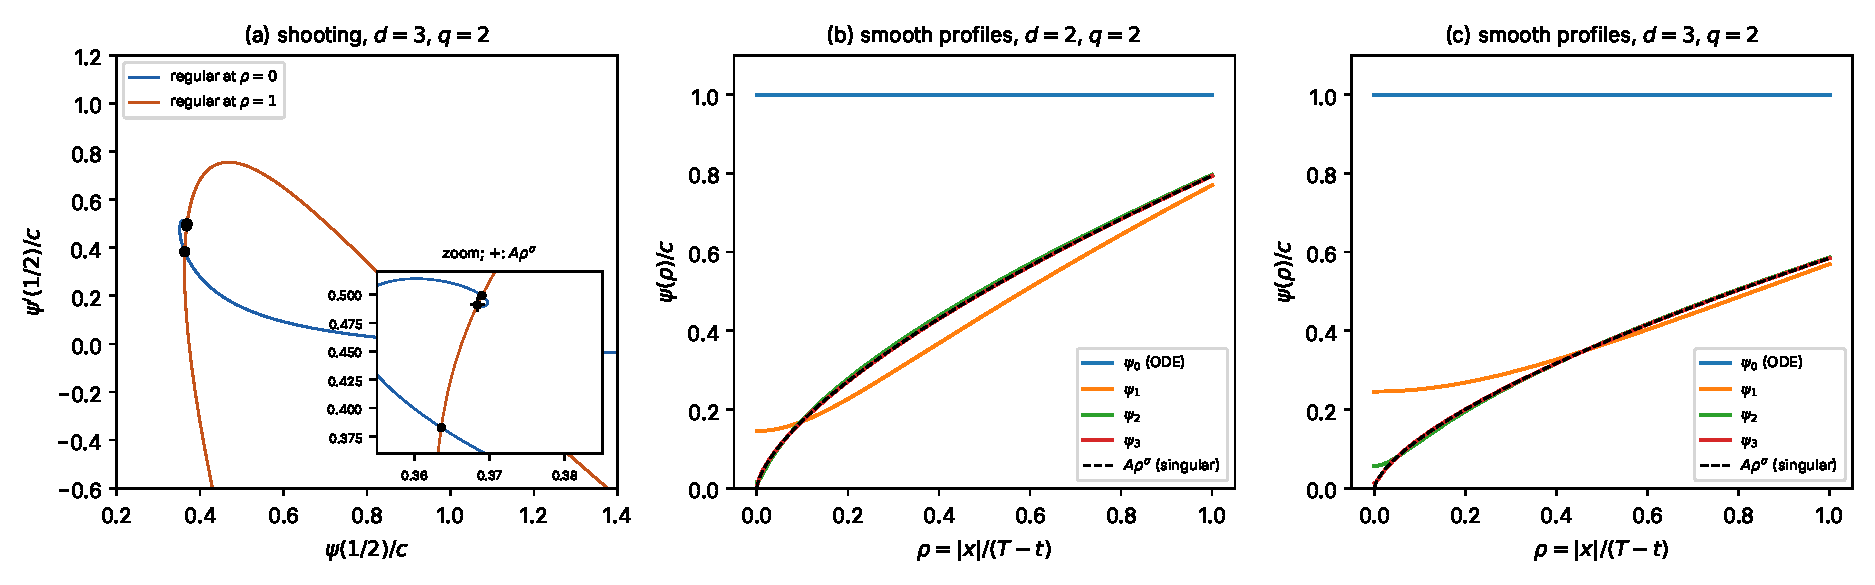
\includegraphics[width=\textwidth]{figures/mems_profile_shooting.pdf}
\caption{(a) Two-sided shooting for $d=3$, $q=2$: the curves of solutions regular
at $\rho=0$ (blue, parametrised by $\psi(0)$) and at $\rho=1$ (orange,
parametrised by $\psi(1)$) in the phase plane at $\rho=\frac12$; intersections
are smooth profiles. The inset shows the spiral of the blue curve around the
singular solution $A\rho^\sigma$. (b), (c) The profiles
$\psi_0\equiv c,\psi_1,\psi_2,\psi_3$ for $d=2,3$, $q=2$, and $A\rho^\sigma$.}
\label{mems:fig-prof}
\end{figure}

\begin{conjecture}\label{mems:conj-prof}
For $d\in\{2,3\}$ and every $q>1$ (more generally whenever $\nu^2>0$),
\eqref{mems:profile-rad} has infinitely many smooth positive solutions
$\psi_n$. They are increasing in $\rho$, and $\psi_n\to\psi_*$ locally
uniformly on $(0,1]$ with $\psi_n(0)/\psi_{n+1}(0)\to e^{\sigma\pi/\nu}$. The
profile $\psi_n$ has exactly $n$ unstable eigenvalues besides those generated by
the symmetries, i.e.\ time and space translations and Lorentz boosts
(\cref{mems:sec-num}). For $d=1$ there are none
(\cref{mems:thm-d1}).
\end{conjecture}

For focusing power nonlinearities, countable families of smooth self-similar
profiles are known \cite{BizonMaisonWasserman2007}, and a proof of
\cref{mems:conj-prof} would presumably follow the same shooting and oscillation
argument. Every $\psi_n$ touches down at the tip with the \emph{same rate}
$(T-t)^{\sigma}$ but a \emph{smaller constant}, $w(t,0)=\psi_n(0)(T-t)^\sigma$
with $\psi_n(0)<c$; the profile is focused at the centre instead of flat.

\subsection{Similarity variables and the free operator}
\label{mems:sec-lin}
With $\psi_1=(T-t)^{-\sigma}w$, $\psi_2=(T-t)^{1-\sigma}\partial_tw$, $T-t=Te^{-\tau}$
(\cref{fw:sec} with $s=-\sigma$), \eqref{mems:eq} becomes
\begin{equation}\label{mems:system}
\partial_\tau\psi_1=-\Lambda\psi_1+\sigma\psi_1+\psi_2,\qquad
\partial_\tau\psi_2=\Delta\psi_1-\Lambda\psi_2-(1-\sigma)\psi_2-\lambda\psi_1^{-q}-\gamma Te^{-\tau}\psi_2 .
\end{equation}
For $\gamma=0$ the static solutions include $\Psi_a=(\psi_a,\Lambda\psi_a-\sigma\psi_a)$, and
$\Psi_0=(c,-\sigma c)$. Writing $\Psi=\Psi_0+\Phi$,
\begin{equation}\label{mems:pert}
  \partial_\tau\Phi=\mathbf L\Phi+\mathbf N(\Phi),\quad
  \mathbf L=\mathbf L_0+\mathbf L',\quad \mathbf L'\Phi=(0,V_0\phi_1),\quad
  \mathbf N(\Phi)=(0,N(\phi_1)),
\end{equation}
where $\mathbf L_0=\mathbf L_0^{(-\sigma)}$ is the free operator of \eqref{fw:system} and
\begin{equation}\label{mems:V0N}
  V_0=q\lambda c^{-q-1}=q\sigma(1-\sigma)=\frac{2q(q-1)}{(q+1)^2},\qquad
  N(\phi)=-\lambda\big[(c+\phi)^{-q}-c^{-q}+qc^{-q-1}\phi\big].
\end{equation}
We work in $\mathcal H^k:=H^k(B^d)\times H^{k-1}(B^d)$, $k\ge2$, and set
$\omega_k:=k-\frac d2-\sigma$. The free operator is \emph{not} dissipative on
low frequencies: polynomial free waves give eigenvalues $\sigma-m$, $m\in\mathbb
N_0$, of $\mathbf L_0$ (e.g.\ $w\equiv1$ gives $(1,0)$ with eigenvalue $\sigma>0$).
The following lemma shows that this is a finite-rank effect. It is a soft
version of the inner-product constructions of
\cite{Ostermann2024,Glogic2025}.

\begin{lemma}[Free operator]\label{mems:lem-free}
Let $k\ge2$ with $\omega_k>0$. There is an inner product $\langle\cdot,\cdot\rangle$
on $\mathcal H^k$, equivalent to the standard one, such that for every
$\varepsilon\in(0,\omega_k)$ there is a finite-rank operator $\mathbf K_\varepsilon$
for which $\mathbf L_0-\mathbf K_\varepsilon$ generates a $C_0$-semigroup with
$\|e^{\tau(\mathbf L_0-\mathbf K_\varepsilon)}\|\le e^{-(\omega_k-\varepsilon)\tau}$.
\end{lemma}

\begin{proof}
\emph{Generation.} For $f\in\mathcal H^k$ extend $f$ to $\mathbb R^d$ (Sobolev
extension), solve the free wave equation and transform back. By finite speed
of propagation this defines a $C_0$-semigroup on $\mathcal H^k$, independent of
the extension, whose generator is the closure of $\mathbf L_0$ on
$C^\infty(\overline{B^d})^2$ (as in
\cite{DonningerSchoerkhuber2017,Ostermann2024}).

\emph{Top order.} For $|\alpha|=k-1$ put $u=\partial^\alpha f$. Since
$[\partial_i,\Lambda]=\partial_i$, $\partial^\alpha\mathbf L_0f$ is the free operator
with $s=-\sigma$ replaced by $s'=-\sigma+k-1$ applied to $u$. Integration by
parts (using $\operatorname{Re}\int_B\nabla u_1\cdot\overline{\nabla\Lambda u_1}=(1-\frac d2)\|\nabla
u_1\|^2+\frac12\int_{\mathbb S^{d-1}}|\nabla u_1|^2$, the analogous identity for
$u_2$, and $\int_B(\nabla u_1\cdot\nabla\bar u_2+\bar u_2\Delta u_1)=\int_{\mathbb S^{d-1}}\bar u_2\,\partial_ru_1$) gives, with $\|f\|_{\dot{\mathcal H}}^2:=\sum_{|\alpha|=k-1}(\|\nabla\partial^\alpha f_1\|^2_{L^2(B)}+\|\partial^\alpha f_2\|^2_{L^2(B)})$,
\begin{equation}\label{mems:energy}
\operatorname{Re}(\mathbf L_0f,f)_{\dot{\mathcal H}}
=-\omega_k\|f\|_{\dot{\mathcal H}}^2-\frac12\sum_{|\alpha|=k-1}\int_{\mathbb S^{d-1}}
\big(|\nabla_{\!T}\partial^\alpha f_1|^2+|\partial_r\partial^\alpha f_1-\partial^\alpha f_2|^2\big)\,dS
\le-\omega_k\|f\|^2_{\dot{\mathcal H}}
\end{equation}
for $f\in C^\infty(\overline{B^d})^2$ ($\nabla_T$ is the tangential gradient). This
is the rigorous form of the heuristic decay rate of \cref{fw:subsec-steps}.

\emph{Low order.} Let $\langle f,g\rangle:=(f,g)_{\dot{\mathcal H}}+(f,g)_{\mathcal
H^{k-1}}$, with $\mathcal H^{k-1}=H^{k-1}\times H^{k-2}$; this is equivalent to
the standard inner product. Since $\mathbf L_0:\mathcal H^k\to\mathcal H^{k-1}$ is
bounded, \eqref{mems:energy} gives
$\operatorname{Re}\langle\mathbf L_0f,f\rangle\le-\omega_k\|f\|^2+C\|f\|\,\|f\|_{\mathcal H^{k-1}}$.
The embedding $J:\mathcal H^k\hookrightarrow\mathcal H^{k-1}$ is compact (Rellich).
So for $\varepsilon>0$ there is a finite-rank orthogonal projection $Q$ in
$\mathcal H^k$ (spectral projection of $J^*J$) with $\|J(I-Q)\|\le\varepsilon/(2C)$.
Then $\|f\|_{\mathcal H^{k-1}}\le\frac{\varepsilon}{2C}\|f\|+\|J\|\|Qf\|$, and
$\operatorname{Re}\langle\mathbf L_0f,f\rangle\le-(\omega_k-\varepsilon)\|f\|^2+C_\varepsilon\|Qf\|^2$.
With $\mathbf K_\varepsilon:=C_\varepsilon Q$, the operator $\mathbf L_0-\mathbf K_\varepsilon+(\omega_k-\varepsilon)$
is dissipative on a core. It is a bounded perturbation of a generator, so
Lumer--Phillips gives the bound \cite[Ch.~II--III]{EngelNagel2000}.
\end{proof}

Since $\mathbf L'$ maps $\mathcal H^k$ into $\{0\}\times H^k\hookrightarrow\{0\}\times H^{k-1}$
compactly, $\mathbf L=(\mathbf L_0-\mathbf K_\varepsilon)+(\mathbf K_\varepsilon+\mathbf L')$
generates a semigroup $\mathbf S(\tau)$, and
$\sigma(\mathbf L)\cap\{\operatorname{Re}\mu>-\omega_k\}$ consists of isolated
eigenvalues of finite algebraic multiplicity (analytic Fredholm theorem;
\cite[IV.5]{Kato1995}, \cite{EngelNagel2000}). In particular the positive free
eigenvalue $\sigma$ is harmless: it is not an eigenvalue of $\mathbf L$.

\subsection{Spectral analysis}
\label{mems:sec-spec}

\begin{proposition}[Spectrum]\label{mems:prop-spec}
Let $k\ge2$ with $\omega_k>0$. A number $\mu$ with $\operatorname{Re}\mu>-\omega_k$ is an
eigenvalue of $\mathbf L$ on $\mathcal H^k$ iff
\begin{equation}\label{mems:eigs}
  \mu\in\{\,1-\ell-2n\,\}\ \cup\ \{\,-(2-2\sigma)-\ell-2n\,\},\qquad \ell,n\in\mathbb N_0,
\end{equation}
($\ell\in\{0,1\}$, the parity, if $d=1$). The eigenfunctions are
$f=(g,(\mu-\sigma+\Lambda)g)$ with $g=|\xi|^\ell Y_\ell(\xi/|\xi|)\,p(|\xi|^2)$,
where $Y_\ell$ is a spherical harmonic and $p$ is a polynomial. The
non-negative eigenvalues are
\begin{itemize}[nosep]
\item $\mu=1$ ($\ell=0$): $f_T=(1,1-\sigma)$, the time-translation mode,
  $\partial_T$ of the rescaled $w^{T,0}$;
\item $\mu=0$ ($\ell=1$, $d$-fold): $f_{L,j}=(\xi_j,(1-\sigma)\xi_j)=(c\sigma)^{-1}\partial_{a_j}\Psi_a|_{a=0}$,
  the Lorentz modes.
\end{itemize}
The largest negative eigenvalues are $\mu=-(2-2\sigma)$ ($\ell=0$, $f_E=(1,\sigma-2)$,
the \emph{energy mode}: the change of $E$ in \cref{mems:prop-ode}(i)) and $\mu=-1$
($\ell=0,n=1$ and $\ell=2,n=0$). Hence the spectral gap is
\begin{equation}\label{mems:gap}
  \omega_0=\min\Big\{1,\ \frac{2(q-1)}{q+1}\Big\}:\qquad
  \omega_0=\tfrac23\ (q=2),\qquad \omega_0=1\ (q\ge3).
\end{equation}
\end{proposition}

\begin{proof}
This is \cref{fw:thm-spec} with $s=-\sigma$; we record the MEMS-specific
points (all identities verified in \texttt{mems\_symbolic\_checks.py}). The
first component of $(\mu-\mathbf L)f=0$ gives $f_2=(\mu-\sigma+\Lambda)f_1$. Then
$f_1=g$ solves \eqref{fw:eig} with $a=\mu-\sigma$, whose characteristic roots
are $a_1=1-\sigma$, $a_2=\sigma-2$ (indeed $1+4V_0=(\frac{3q-1}{q+1})^2$). By interior
elliptic regularity $g\in C^\infty(B^d)$. Its projections
$G_{\ell m}(r)=\int_{\mathbb S^{d-1}}g(r\omega)\overline{Y_{\ell m}(\omega)}d\omega$ lie in
$H^k(\frac12,1)$ and are $O(r^\ell)$ at $0$, hence $G_{\ell m}=\mathrm{const}\cdot
r^\ell{}_2F_1(\alpha,\beta;\ell+\frac d2;r^2)$ with
$\alpha=\frac{\mu-1+\ell}{2}$, $\beta=\frac{\mu+2-2\sigma+\ell}{2}$. (For $d=1$ the
second solution at $0$ has the opposite parity.) At $z=1$ the exponents are
$0$ and $\delta(\mu)=\frac{d-1}2+\sigma-\mu$, and
$\operatorname{Re}\mu>-\omega_k\iff\operatorname{Re}\delta<k-\frac12$. Hence
$(1-z)^{\delta}$ ($\delta\notin\mathbb Z$), $(1-z)^{m}\log(1-z)$ ($\delta=m\in\mathbb N_0$)
and $(1-z)^{-m}$ ($\delta=-m<0$) are not in $H^k$ near $z=1$. In all three
cases the coefficient of the offending term in the connection formula
\cite[15.8]{DLMF} is a nonzero multiple of $1/(\Gamma(\alpha)\Gamma(\beta))$.
Therefore $\alpha\in-\mathbb N_0$ or $\beta\in-\mathbb N_0$, and conversely these
give polynomial (hence admissible) eigenfunctions. The possibility that
\emph{both} Frobenius solutions at $z=1$ are smooth arises only for
$\delta=m\in\mathbb N$ with $(\alpha)_m(\beta)_m=0$, which is again covered by
$\alpha$ or $\beta\in-\mathbb N_0$. Since the solution regular at $0$ is
unique up to a factor, each harmonic $Y_{\ell m}$ contributes at most one
eigenfunction. The two families overlap only if $\alpha-\beta=\sigma-\frac32\in\mathbb Z$,
i.e.\ for $q=3$ (\cref{mems:rem-q3}). Solving $\alpha=-n$, $\beta=-n$ gives \eqref{mems:eigs}. The physical
identification follows from \cref{mems:lem-sym}, and from the spatially
homogeneous perturbations $(T-t)^{\sigma-1}$ and $(T-t)^{2-\sigma}$ of the ODE
(roots of $m(m-1)=V_0$), which correspond to $\mu=1$ and $\mu=-(2-2\sigma)$.
\end{proof}

\begin{lemma}[Semisimplicity]\label{mems:lem-jordan}
Let $d\le3$ and let $k\ge2$ with $\omega_k>0$. Then $(1-\mathbf L)g=f_T$ and
$(-\mathbf L)g=f_{L,j}$ have no solution $g\in\mathcal D(\mathbf L)$. Consequently the
Riesz projections $\mathbf P_1$ (at $\mu=1$) and $\mathbf P_0$ (at $\mu=0$) have
ranks $1$ and $d$, with $\operatorname{ran}\mathbf P_1=\langle f_T\rangle$ and
$\operatorname{ran}\mathbf P_0=\langle f_{L,1},\dots,f_{L,d}\rangle$.
\end{lemma}

\begin{proof}
$(\mu-\mathbf L)g=f$ is equivalent to $g_2=(a+\Lambda)g_1-f_1$ and
$-\big[(\delta_{ij}-\xi_i\xi_j)\partial_{ij}g_1-2(a+1)\Lambda g_1-(a(a+1)-V_0)g_1\big]=f_2+(a+1)f_1+\Lambda f_1$.
For $f=f_T$ ($a=1-\sigma$, so $a(a+1)=V_0$) the right side is $3-2\sigma$; for
$f=f_{L,j}$ ($a=-\sigma$) it is $(3-2\sigma)\xi_j$. With $g_1=G(r)$, resp.\
$g_1=rK(r)\xi_j/|\xi|$, both reduce to the first-order equation
\[
  (1-r^2)P'+\Big(\frac{D-1}{r}-2(2-\sigma)r\Big)P=-(3-2\sigma),\qquad P=G'\ (D=d),\quad P=K'\ (D=d+2).
\]
The solution regular at $r=0$ is
$P=-(3-2\sigma)r^{1-D}(1-r^2)^{-(e+1)}\int_0^r s^{D-1}(1-s^2)^{e}ds$ with
$e=\frac{3-D}2-\sigma$. Near $r=1$,
$\int_0^r s^{D-1}(1-s^2)^e\,ds=C_D+(1-r^2)^{e+1}A(r)$ with $A$ analytic and
\[
  C_D=\frac{\Gamma(\frac D2)\,\Gamma(e+1)}{2\,\Gamma(\frac52-\sigma)}\neq0
\]
(analytic continuation of the Beta integral when $e<-1$). The only exception
is $e+1\in-\mathbb N_0$, which for $d\le3$ happens only for $D=4$, $q=3$, where a
term $\log(1-r^2)$ with coefficient $-\frac12$ appears instead. Hence $g_1$
contains $C\,(1-r)^{\delta(\mu)}$ with $C\ne0$ and $\delta(1)=\frac{d-3}2+\sigma$,
$\delta(0)=\frac{d-1}2+\sigma$. Both are non-integers for $d\le3$, except for
$(d,q)=(2,3)$, where $\delta(1)=0$ and $\delta(0)=1$ and one gets $\log(1-r)$,
resp.\ $(1-r)\log(1-r)$, instead. As
$\delta(\mu)<k-\frac12$, $g_1\notin H^k$. (The constant $C_D$ and the expansion
were checked numerically with \texttt{mpmath}.)
\end{proof}

\begin{remark}[$q=3$: a Jordan block at the gap]\label{mems:rem-q3}
For $q=3$ the two families in \eqref{mems:eigs} collide at $\mu=-1=-\omega_0$ in the
sector $\ell=0$, with the single eigenfunction $f_E=(1,-\frac32)$. In this case
$(-1-\mathbf L)g=f_E$ \emph{is} solvable with
$g=(|\xi|^2/d,\ |\xi|^2/(2d)-1)$, so $\mu=-1$ carries a Jordan block (verified
symbolically; in the collocation of \cref{mems:sec-num} this double eigenvalue
splits by $\approx10^{-5}$, much more than the errors for simple eigenvalues). Hence for van der Waals forces the decay at the
rate $\omega_0=1$ fails by a factor $\tau$, which matches the $\theta\log\theta$
term in \eqref{mems:dampedexp} below. This does not affect
\cref{mems:thm-main}, where $\omega<\omega_0$.
\end{remark}

\begin{proposition}[Linear stability]\label{mems:prop-lin}
Let $d\le3$, $k\ge2$, $\omega_k>0$, and $\mathbf P=\mathbf P_1+\mathbf P_0$. Then
$\mathbf S(\tau)\mathbf P_1=e^\tau\mathbf P_1$, $\mathbf S(\tau)\mathbf P_0=\mathbf P_0$, and for every
$\omega<\min\{\omega_0,\omega_k\}$ there is $M_\omega$ with
$\|\mathbf S(\tau)(\mathbf I-\mathbf P)f\|\le M_\omega e^{-\omega\tau}\|(\mathbf I-\mathbf P)f\|$.
\end{proposition}

\begin{proof}
Fix $\omega<\omega'<\min\{\omega_0,\omega_k-\varepsilon\}$. On $\operatorname{Re}\mu\ge-\omega'$,
$\mathbf R_{\mathbf L}(\mu)=\mathbf R_0(\mu)[\mathbf I-(\mathbf K_\varepsilon+\mathbf L')\mathbf R_0(\mu)]^{-1}$ with
$\mathbf R_0$ the resolvent of $\mathbf L_0-\mathbf K_\varepsilon$. Here
$\|\mathbf L'\mathbf R_0(\mu)\|\lesssim|\mu|^{-1}$. Indeed, $u=\mathbf R_0(\mu)f$
satisfies $\mu u_1=f_1-\Lambda u_1+\sigma u_1+u_2+(\mathbf K_\varepsilon u)_1$, so
$\|u_1\|_{H^{k-1}}\lesssim|\mu|^{-1}\|f\|$. Also
$\|\mathbf K_\varepsilon\mathbf R_0(\mu)\|\to0$ as $|\mu|\to\infty$: write $\mathbf K_\varepsilon$
via vectors in the dense set $\mathcal D(\mathbf L_0^*)$, up to a small error.
Hence $\mathbf R_{\mathbf L}$ is uniformly bounded for $|\mu|$ large. On the
remaining compact set it is analytic except at $\mu=1,0$
(\cref{mems:prop-spec}). The Gearhart--Prüss theorem
\cite[V.1.11]{EngelNagel2000} applied to $\mathbf L|_{\operatorname{ran}(\mathbf I-\mathbf P)}$
gives the bound. \Cref{mems:lem-jordan} gives the action on $\operatorname{ran}\mathbf P$.
\end{proof}

\paragraph{Required regularity.} To see the full gap one needs $\omega_k\ge\omega_0$,
i.e.\ $k\ge\frac d2+\sigma+\omega_0$, together with $k>\frac d2$ (for the
nonlinearity) and $k\ge2$. Since $\sigma+\omega_0=\min\{1+\sigma,2-\sigma\}\le\frac32$,
\[
  k=2\ (d=1),\qquad k=3\ (d=2,3)\qquad\text{suffice for every }q>1 .
\]
For $(d,q)=(1,3),(3,3)$ the value $\omega_k=\omega_0=1$ is attained exactly, which is
harmless since $\omega<\omega_0$. For smaller admissible $k$ (e.g.\ $k=2$, $d=2$) everything
holds with $\omega<\min\{\omega_0,\omega_k\}$.

\subsection{Nonlinear stability of ODE touchdown}
\label{mems:sec-nonlin}
Normalise $T_0=1$ by scaling. The reference solution $w^{1,0}=c(1-t)^\sigma$ has
data $(c,-\sigma c)$ at $t=0$.

\begin{theorem}[Stable self-similar touchdown]\label{mems:thm-main}
Let $\gamma=0$, $q>1$, $\lambda>0$, $d\in\{1,2,3\}$, $k=2$ if $d=1$ and $k=3$ if
$d=2,3$, and $0<\omega<\omega_0=\min\{1,\frac{2(q-1)}{q+1}\}$. There are
$\delta>0$, $M\ge1$ such that the following holds. Let real data
$(w_0,w_1)=(c,-\sigma c)+(v_0,v_1)$ satisfy
$\|(v_0,v_1)\|_{H^k\times H^{k-1}(B_{1+\delta})}\le\delta/M$. Then there exist
$T^*\in[1-\delta,1+\delta]$ and $a^*\in\mathbb R^d$, $|a^*|\le\delta$, such that the
solution $w$ of \eqref{mems:eq} with these data exists in the backward cone
$\Gamma_{T^*}$, is positive there, touches down at $(T^*,0)$, and satisfies, for
$0\le t<T^*$,
\begin{align*}
  (T^*-t)^{|\alpha|-\sigma-\frac d2}\big\|\partial_x^\alpha\big(w(t)-w^{T^*,a^*}(t)\big)\big\|_{L^2(B_{T^*-t})}&\lesssim\delta\,(T^*-t)^{\omega},\quad|\alpha|\le k,\\
  (T^*-t)^{|\alpha|+1-\sigma-\frac d2}\big\|\partial_x^\alpha\partial_t\big(w(t)-w^{T^*,a^*}(t)\big)\big\|_{L^2(B_{T^*-t})}&\lesssim\delta\,(T^*-t)^{\omega},\quad|\alpha|\le k-1.
\end{align*}
In particular, uniformly for $|x|\le T^*-t$,
\begin{gather*}
  w(t,x)=(T^*-t)^{\sigma}\Big[\psi_{a^*}\Big(\frac{x}{T^*-t}\Big)+O\big(\delta(T^*-t)^{\omega}\big)\Big],\\
  \partial_tw(t,0)=-\sigma c\,(1-|a^*|^2)^{-\frac\sigma2}(T^*-t)^{\sigma-1}\big(1+O((T^*-t)^{\omega})\big).
\end{gather*}
If the data are radial (even, if $d=1$), then $a^*=0$.
\end{theorem}

\begin{proof}[Proof sketch]
\emph{1. Data and unknowns.} For $T\in[1-\delta,1+\delta]$ and $|a|\le\delta$, the
rescaled data are $\mathbf U(v,T)=(T^{-\sigma}w_0(T\cdot),T^{1-\sigma}w_1(T\cdot))$ on
$B^d$ ($B_T\subset B_{1+\delta}$). We write $\Psi(\tau)=\Psi_a+\Phi(\tau)$, so that
$\Phi(0)=\mathbf u(T,a):=\mathbf U(v,T)-\Psi_a$ and
\[
  \partial_\tau\Phi=\mathbf L\Phi+\mathbf G_a(\Phi),\qquad
  \mathbf G_a(\Phi)=\big(0,\ (V_a-V_0)\phi_1+N_a(\phi_1)\big),
\]
with $V_a=q\lambda\psi_a^{-q-1}$, $\|V_a-V_0\|_{C^k(\overline B)}\lesssim|a|$,
and $N_a(\phi)=-\lambda[(\psi_a+\phi)^{-q}-\psi_a^{-q}+q\psi_a^{-q-1}\phi]$.

\emph{2. Nonlinearity.} As $k>\frac d2$, $H^k(B^d)$ is an algebra and
$\|\phi\|_{L^\infty}\le C_k\|\phi\|_{H^k}$. For $\|\phi\|_{H^k}\le\delta$ with $C_k\delta\le c/4$
we have $\psi_a+\phi\ge c/4$ on $\overline{B^d}$, i.e.\ the solution stays away from
the singularity of $w^{-q}$, and $N_a(\phi)=\phi^2\int_0^1(1-\theta)F''(\psi_a+\theta\phi)\,d\theta$ with
$F(w)=-\lambda w^{-q}$ smooth on $[c/4,\infty)$. Moser estimates give
$\|N_a(\phi)-N_a(\tilde\phi)\|_{H^{k-1}}\lesssim(\|\phi\|_{H^k}+\|\tilde\phi\|_{H^k})\|\phi-\tilde\phi\|_{H^k}$.

\emph{3. Modified Duhamel equation.} In
$\mathcal X=\{\Phi\in C([0,\infty),\mathcal H^k):\|\Phi\|_{\mathcal X}:=\sup_\tau e^{\omega\tau}\|\Phi(\tau)\|\le\delta\}$ solve
\begin{gather*}
  \Phi(\tau)=\mathbf S(\tau)\big[\mathbf u-\mathbf C(\Phi,\mathbf u)\big]+\int_0^\tau\mathbf S(\tau-\tau')\mathbf G_a(\Phi(\tau'))\,d\tau',\\
  \mathbf C(\Phi,\mathbf u)=\mathbf P\mathbf u+\int_0^\infty\big(e^{-\tau'}\mathbf P_1+\mathbf P_0\big)\mathbf G_a(\Phi(\tau'))\,d\tau'.
\end{gather*}
By Step 2, $\|\mathbf G_a(\Phi)(\tau)\|\lesssim(\delta^2+|a|\delta)e^{-\omega\tau}$, with the
corresponding Lipschitz bound. By \cref{mems:prop-lin}, the
right-hand side maps $\mathcal X$ into itself and is a contraction, provided
$\|(\mathbf I-\mathbf P)\mathbf u\|\le\delta/(2M_\omega)$. This holds because
$\mathbf u(T,a)=[\mathbf U(0,T)-\Psi_0]+[\Psi_0-\Psi_a]+[\mathbf U(v,T)-\mathbf U(0,T)]$, with
\[
  \mathbf U(0,T)-\Psi_0=-c\sigma(T-1)f_T+O((T-1)^2),\qquad
  \Psi_0-\Psi_a=-c\sigma\,a\cdot f_L+O(|a|^2),
\]
so $\|(\mathbf I-\mathbf P)\mathbf u\|\lesssim\delta/M+\delta^2$. The fixed point $\Phi_{T,a}$ is
continuous in $(T,a)$.

\emph{4. Choice of $(T^*,a^*)$.} In the basis $f_T,f_{L,1},\dots,f_{L,d}$ of
$\operatorname{ran}\mathbf P$,
$\mathbf C(\Phi_{T,a},\mathbf u(T,a))=-c\sigma\big((T-1)f_T+a\cdot f_L\big)+\mathbf R(T,a)$ with
$\mathbf R$ continuous and $|\mathbf R|\lesssim\delta/M+\delta^2$. (The terms are
exactly the symmetry generators, \cref{mems:prop-spec}.) By Brouwer's fixed
point theorem there is $(T^*,a^*)\in[1-\delta,1+\delta]\times\overline{B_\delta}$ with
$\mathbf C=0$, for $M$ large and $\delta$ small. Then $\Phi$ solves the true Duhamel
equation. For radial data everything can be done in the radial subspace,
where $\mathbf P_0=0$, so $a^*=0$.

\emph{5. Back to $w$.} The mild solution coincides with the (strong) solution of
\eqref{mems:eq} in $\Gamma_{T^*}$ (approximation by smooth data and finite
speed of propagation). Since $\psi_1=\psi_{a^*}+\phi_1$ and
$\|\phi_1(\tau)\|_{L^\infty}\lesssim\delta e^{-\omega\tau}$, $w>0$ in the cone and $w(t,0)\to0$.
The estimates are $\|\Phi(\tau)\|_{\mathcal H^k}\le\delta e^{-\omega\tau}$ rewritten
with $e^{-\tau}=(T^*-t)/T^*$. The formula for $\partial_tw(t,0)$ uses
$H^{k-1}\hookrightarrow C^0$, which holds since $k-1>\frac d2$ for our
choices of $k$.
\end{proof}

\begin{remark}\label{mems:rem-main}
(a) \emph{No translation parameter is needed.} The ODE profile is
translation invariant, and $w^{T,a}(\cdot,\cdot-x_0)=w^{T-a\cdot x_0,a}$. Applying
the theorem at every nearby base point $x_0$ (translated data) shows that,
near $x_0=0$, touchdown happens along a hypersurface $t=T^*(x_0)$. For the
exact solutions $a=\nabla T^*$. We expect $a^*=\nabla T^*(0)$ and $T^*\in C^1$
in general, as for the 1D power case \cite{MerleZaag2007}; we have not proved it.
(b) The rate $\omega_0=\frac23$ for $q=2$ is dictated by the ODE energy mode
$\mu=-(2-2\sigma)$. For $q\ge3$ it is the PDE mode $\mu=-1$, which by
\cref{mems:rem-q3} is not semisimple when $q=3$.
(c) The theorem is in the style of
\cite{DonningerSchoerkhuber2016,DonningerSchoerkhuber2017,Ostermann2024}.
The new features are $s<0$ (\cref{mems:lem-free}) and the need to keep the
solution away from $w=0$, which the $L^\infty$ control from $k>\frac d2$
provides.
\end{remark}

\subsection{Damping and other integrable perturbations}
\label{mems:sec-damp}
In \eqref{mems:system}, damping contributes $-\gamma Te^{-\tau}\psi_2$, a perturbation
decaying at rate $1\ge\omega_0$. Exact self-similar solutions no longer exist
(there is no scaling symmetry), but the touchdown remains asymptotically
self-similar.

\paragraph{Damped ODE.} For $W''+\gamma W'=-\lambda W^{-q}$, inserting
$W=c\theta^\sigma(1+c_1\theta+\dots)$, $\theta=T-t$, the $\theta^{\sigma-1}$-terms give
$c_1\sigma(3-q)=\gamma\sigma$. Including the free energy mode,
\begin{equation}\label{mems:dampedexp}
  W=c\,\theta^\sigma\Big(1+e\,\theta^{2-2\sigma}+\frac{\gamma}{3-q}\,\theta+\dots\Big)\ (q\ne3),\qquad
  W=c\,\theta^{1/2}\Big(1+\frac{\gamma}{4}\,\theta\log\theta+e\,\theta+\dots\Big)\ (q=3).
\end{equation}
For $q=2$, $c_1=\gamma$. For $q<3$ the damping correction is positive (larger gap at
the same remaining time and the same $e$); for $q>3$ it is negative. For $q=3$ the exponents $1$ and $2-2\sigma$ resonate. Both formulas are
confirmed numerically (fitted coefficients within $0.4\%$ of the predicted ones;
\texttt{mems\_damped\_ode.py}). In
similarity variables the background is $\Psi_0+O(\gamma Te^{-\tau})$ (or
$O(\gamma T\tau e^{-\tau})$ if $q=3$).

\begin{proposition}[Damped touchdown, sketch]\label{mems:prop-damped}
Assume the hypotheses of \cref{mems:thm-main}, except that the damping
satisfies $0\le\gamma\le\delta/M$, i.e.\ $\gamma T_0\le\delta/M$ in general units.
Then the conclusions of \cref{mems:thm-main} hold verbatim, for radial and
nonradial data, with the same comparison profiles $w^{T^*,a^*}$.
\end{proposition}

\begin{proof}[Sketch]
Add $-\gamma Te^{-\tau}(0,\psi_{a,2}+\phi_2)$ to $\mathbf G_a$. Its size is
$\lesssim\gamma e^{-\tau}\le\gamma e^{-\omega\tau}$, its Lipschitz constant is $\lesssim\gamma$, and
$\int_0^\tau e^{-\omega'(\tau-\tau')}e^{-\tau'}d\tau'\lesssim e^{-\omega\tau}$ since $\omega<\omega'<\omega_0\le1$.
Steps 3--5 go through with $\delta^2+|a|\delta$ replaced by
$\delta^2+|a|\delta+\gamma$. The key point for the nonradial case is that the
neutral component obeys $\frac{d}{d\tau}\mathbf P_0\Phi=\mathbf P_0\mathbf G_a(\Phi)$
(no Jordan block). The right side is \emph{integrable} in $\tau$, so
$\mathbf P_0\Phi(\tau)$ has a limit, and the static choice of $a$ by Brouwer makes it
zero. A dynamical modulation of the boost (cf.\ \cref{fw:subsec-lower}) would
be needed only for a non-integrable forcing of the neutral modes.
\end{proof}

\begin{corollary}[Arbitrary damping; sketch]\label{mems:cor-damped}
Let $\gamma\ge0$ and let $W$ be any solution of the damped ODE that touches down at
$T_0>0$. Then data close enough to $(W(0),W'(0))$ in
$H^k\times H^{k-1}(B_{T_0+\eta})$ lead to touchdown at $(T^*,0)$, $T^*\to T_0$ as
the data converge, with the asymptotics of \cref{mems:thm-main}.
\end{corollary}

\begin{proof}[Sketch]
By \eqref{mems:dampedexp}, at $t_1=T_0-\theta_1$ the rescaled data of $W$ differ
from $(c,-\sigma c)$ by $O(\theta_1^{\min\{1,2-2\sigma\}})$ (times $\log$ if $q=3$), and the
rescaled damping is $\gamma\theta_1$. Choose $\theta_1$ so small that both are
$\le\delta/(2M)$. By local well-posedness and continuous dependence on
$[0,t_1]$ (the solution stays near $W(t)\ge W(t_1)>0$), data close enough to
those of $W$ produce data at $t_1$ satisfying the hypotheses of
\cref{mems:prop-damped} after rescaling by $\theta_1$.
\end{proof}

The same argument covers any perturbation that is $O(e^{-\tau})$ in similarity
variables. For instance a smooth dielectric profile $f(x)>0$ in
$-\lambda f(x)w^{-q}$ gives
$\lambda f(Te^{-\tau}\xi)\psi_1^{-q}=\lambda f(0)\psi_1^{-q}+O(e^{-\tau})$.
Touchdown at a point $x_0$ is then ODE-like with $c=c(\lambda f(x_0))$. This is
not written out.

\subsection{Physical interpretation}
\label{mems:sec-phys}
\begin{itemize}[leftmargin=1.2em]
\item \emph{Rate and impact speed.} For the Coulomb force ($q=2$) the gap
closes like $w\approx(9\lambda/2)^{1/3}(T-t)^{2/3}$, i.e.\
$1+u\approx(9\lambda/2)^{1/3}\big((T-t)/\varepsilon\big)^{2/3}$ in the original time.
The impact speed $u_t\sim-\frac23(9\lambda/2)^{1/3}\varepsilon^{-2/3}(T-t)^{-1/3}$
is infinite. In the parabolic model ($\varepsilon=0$) the ODE
$W'=-\lambda W^{-2}$ gives instead $w\approx(3\lambda(T-t))^{1/3}$; for the
rigorous parabolic theory see \cite{EspositoGhoussoubGuo2010} and references
therein.
% TODO verify and cite Guo--Pan--Ward, SIAM J. Appl. Math. 66 (2005) for the parabolic rate (T-t)^{1/3}.
For $\varepsilon>0$, inertia dominates damping once
$T-t\ll\varepsilon^2/\gamma$ (the scale-invariant damping is $\gamma(T-t)/\varepsilon^2$).
Hence the \emph{final} touchdown asymptotics is the hyperbolic one,
\cref{mems:cor-damped}, and the parabolic rate is at most an intermediate
regime for $\varepsilon^2\ll T-t\ll1$.
\item \emph{Flat profile, touchdown on a hypersurface.} The stable profile is
constant in the light cone. Near touchdown the gap closes uniformly over a
region of size $\sim T-t$ (in units of the wave speed), and the touchdown set
is locally a spacelike hypersurface $t=T^*(x)$
(\cref{mems:rem-main}(a)). This differs sharply from parabolic MEMS, where
touchdown is typically at isolated points. The focused profiles $\psi_n$ of
\cref{mems:conj-prof} touch down at a point but are unstable.
\item \emph{Locality.} Only data in the base of the cone, $B_{T^*}(x_0)$, matter.
The clamped boundary, the shape of $\Omega$ and the far-away dielectric profile are
irrelevant as long as this ball lies inside $\Omega$.
\item \emph{An explicit scenario.} Release the undamped device ($q=2$) from rest,
$w\equiv1$, $w_t\equiv0$, and let $B_R(x_0)\subset\Omega$. By finite speed of
propagation $w(t,x)=W(t)$ for $|x-x_0|<R-t$. If
$T_0=\pi/(2\sqrt{2\lambda})<R$, i.e.\ $\lambda>\pi^2/(8R^2)$, the membrane therefore
touches down \emph{simultaneously on the ball} $|x-x_0|<R-T_0$ (unless it has
quenched elsewhere earlier; we have not excluded this). By
\cref{mems:thm-main,mems:prop-damped} this flat touchdown is stable under
small perturbations of the data, of the damping and of the permittivity. It
then occurs on a nearby spacelike hypersurface with a boosted ODE profile.
For $R=1$ the threshold $\pi^2/8\approx1.234$ should be compared with the
static pull-in values $\lambda^*\approx0.350$ (interval $(-1,1)$), $0.789$ (unit
disk) and $1.299$ (unit ball in $\mathbb R^3$) (\texttt{mems\_damped\_ode.py}).
\item \emph{Dimensions.} $d=1$ describes strings and membrane strips (beams with
bending stiffness, $\Delta^2$, are \emph{not} covered: there is no light cone);
$d=2$ describes the membrane (e.g.\ a disk); $d=3$ is included for comparison
with the wave-equation literature.
\end{itemize}

\subsection{Numerical checks}
\label{mems:sec-num}
The eigenvalue problem in the sector $\ell$ is the quadratic pencil
$z(1-z)h''+(\ell+\frac d2-(b+\frac32)z)h'-\frac14(b^2+b-V)h=0$,
$b=\mu-\sigma+\ell$, $g=|\xi|^\ell Y_\ell h(|\xi|^2)$. We solved it by Chebyshev
collocation in $z\in[0,1]$ without boundary conditions, keeping eigenvalues
that are stable under refinement ($N=20,28$; larger $N$ starts to resolve the
non-smooth generalised eigenfunctions of $\operatorname{Re}\mu\le-\omega_k$ and produces
spurious eigenvalues). For $V\equiv V_0$, $q=2,3,4$, $d=1,2,3$ and
$\ell\le2$, all eigenvalues with $\operatorname{Re}\mu>-1.9$ agree with
\eqref{mems:eigs} to $\le10^{-5}$. No others appear. For $q=3$ the double
eigenvalue $-1$ splits as expected for a Jordan block. An independent
discretisation of the full first-order operator $\mathbf L$ for $d=1$ gives
$\{1,0,-\frac23,-1,-\frac53\}$ for $q=2$ (both parities), as predicted.
For the excited profiles ($d=3$, $q=2$, $V=q\lambda\psi_n^{-q-1}$) we find:
\begin{itemize}[nosep]
\item $\psi_1$: $\{3.4955,\,1\}$ for $\ell=0$; $\{1,\,0\}$ for $\ell=1$ (space
translation, which is non-trivial for a non-constant profile, and boost); none
for $\ell=2$.
\item $\psi_2$: $\{20.35,\,3.598,\,1\}$ for $\ell=0$ (this needs $N\ge120$).
\end{itemize}
Thus $\psi_1$ has one and $\psi_2$ two genuinely unstable directions, as in
\cref{mems:conj-prof}. See \cref{mems:fig-spec}
(\texttt{mems\_spectrum\_numerics.py}). The independent numerics section of this
note provides a further check.

\begin{figure}[ht]
\centering
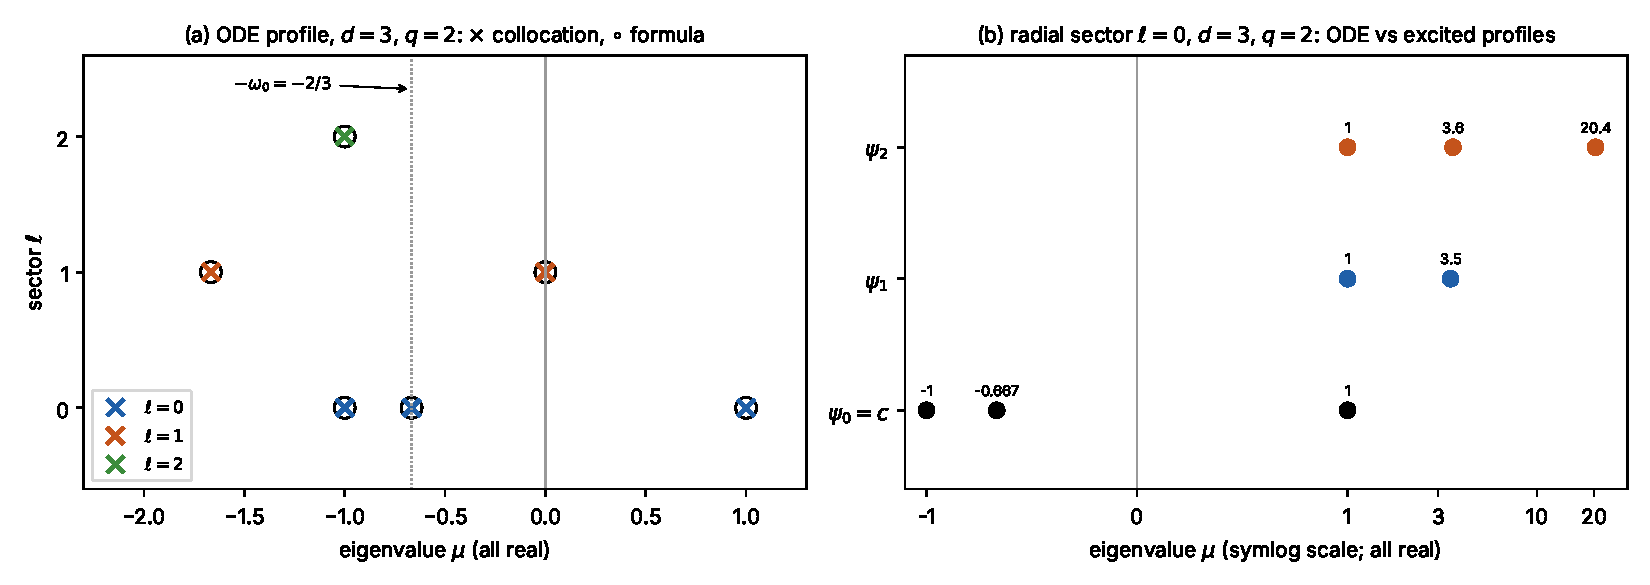
\includegraphics[width=\textwidth]{figures/mems_spectrum.pdf}
\caption{(a) Eigenvalues of the linearisation at the ODE profile, $d=3$, $q=2$,
sectors $\ell=0,1,2$: collocation ($\times$) versus \eqref{mems:eigs} ($\circ$);
the dotted line is $-\omega_0=-\frac23$ (energy mode). (b) Radial eigenvalues
($\operatorname{Re}\mu>-0.3$ for $\psi_{1,2}$) of the ODE profile $\psi_0=c$ and of the
first two excited profiles: $\psi_n$ has $n$ unstable eigenvalues in addition to
the time-translation eigenvalue $1$.}
\label{mems:fig-spec}
\end{figure}

\subsection{Relation to Gimperlein--He--Lacey}
\label{mems:sec-ghl}
The closest prior work is \cite{GimperleinHeLacey2022} (see also
\cite{He2021}). According to the summary in \cref{lit:mems}, it studies the
self-similar quenching of \eqref{lit:eq:memsq} formally and numerically:
\begin{itemize}[nosep]
\item it treats the ODE profile $\kappa_q(T-t)^{2/(q+1)}$;
\item it obtains formally a sequence of self-similar solutions;
\item it gives evidence that radial solutions increasing in $|x|$ quench at the
origin, that the trivial profile is stable up to time translation, and that the
non-trivial ones are unstable.
\end{itemize}
\emph{Caveat: the text of \cite{GimperleinHeLacey2022} could not be consulted
while this section was written (no network access). The points below compare
with that summary only, and should be checked against the paper.}
% TODO (R. He): check the comparison below against arXiv:2210.14821.
\begin{enumerate}[label=(\alph*),nosep]
\item \emph{Profile and constant.} $\kappa_q=c$, with
$c^{q+1}=\lambda(q+1)^2/(2(q-1))$, \eqref{lit:eq:memsode}.
\item \emph{Non-trivial profiles.} Our $\psi_n$
(\cref{mems:tab-prof}) are increasing in $|x|$ and accumulate at the
\emph{static} singular solution $A|x|^{2/(q+1)}$. The ratio law
$\psi_n(0)/\psi_{n+1}(0)\to e^{\sigma\pi/\nu}$ gives a sharp quantitative test for
identifying them with the sequence of \cite{GimperleinHeLacey2022}.
\Cref{mems:thm-d1} shows that the sequence has no counterpart in $d=1$.
\item \emph{Stability.} We make the stability of the ODE profile rigorous:
modulo time translation for radial data and modulo time translation plus
Lorentz boosts in general (\cref{mems:thm-main}), with damping
(\cref{mems:prop-damped,mems:cor-damped}). We also give the decay rate
$(T-t)^{\omega}$, $\omega<\min\{1,\frac{2(q-1)}{q+1}\}$, and identify the slowest
stable mode as the ODE energy mode for $q<3$. The numerically computed extra
unstable eigenvalues of $\psi_1,\psi_2$ support the instability of the
non-trivial profiles.
\end{enumerate}

\subsection{Caveats and open points}
\label{mems:sec-gaps}
\begin{enumerate}[nosep]
\item \Cref{mems:thm-main,mems:prop-damped,mems:cor-damped} are proof sketches.
The standard parts are referenced, not reproduced: generation of
$\mathbf L_0$ on $\mathcal H^k$, equivalence of mild and strong solutions,
continuity of the fixed point in $(T,a)$, and Moser estimates.
\Cref{mems:lem-free,mems:prop-spec,mems:lem-jordan} are complete modulo
routine details. \Cref{mems:lem-jordan} is stated for $d\le3$; the general
case needs the same Beta-function check.
\item The statements are local in the backward cone. Which points touch down
first, the regularity of the touchdown hypersurface, $a^*=\nabla T^*$, and
the behaviour outside the cone are open.
\item The existence of the non-trivial profiles for $d\ge2$ is numerical
(\cref{mems:conj-prof}); their spectra are low-precision numerics.
Nonradial non-trivial profiles were not searched for.
\item For $q=3$ the eigenvalue $-\omega_0$ is a Jordan block
(\cref{mems:rem-q3}), so the rate $\omega_0=1$ itself is not attained.
\item Not covered: plate models with $\Delta^2$, and nonlocal (series
capacitor) models. In the latter the coefficient
$\lambda(1+\alpha\int w^{-1})^{-2}$ depends on the whole solution, and a flat
touchdown on a set of positive measure would drive it to $0$ (heuristic, not
analysed).
\end{enumerate}

\section{Hyperbolic thermal explosion: exponential nonlinearities}
\label{therm:sec}

In fast thermal processes (pulsed laser heating and processing, ignition of
solid propellants and energetic materials, rapid combustion) the relevant time
scales can approach the thermal relaxation time of the medium, and Fourier's law
is replaced by the Maxwell--Cattaneo--Vernotte (MCV) law
\cite{Cattaneo1958,Vernotte1958,JosephPreziosi1989,Straughan2011}.  Combined
with the Frank-Kamenetskii (FK) exothermic source
\cite{FrankKamenetskii1955,BebernesEberly1989}, this produces damped wave
equations with exponential nonlinearities.  The main points of this section are:
\begin{enumerate}[label=(\arabic*),leftmargin=2em]
\item There are two inequivalent hyperbolic models (``reduced'' and ``full'');
  their blowup is \emph{qualitatively different}.
\item Reduced model: the ODE blowup $\theta\simeq\log(2\tau_*/\delta)-2\log(T-t)$ is
  stable modulo time translation and Lorentz boosts; the linearised spectrum is
  explicit, the spectral gap is $1$ (\cref{therm:thm:reduced}).
\item In $d=1$ the reduced model is Liouville's equation; the explicit general
  solution confirms the theorem, including the sharpness of the gap
  (\cref{therm:sec:liouville}).
\item Full (MCV-consistent) model: the blowup is $\theta\simeq-\log\bigl(\delta(T-t)\bigr)$ (the
  \emph{parabolic} rate) with a \emph{hyperbolic} spatial structure; there is no
  Lorentz invariance, the neutral modes come from a family of tilted plane
  waves, and $\lambda=-1$ carries a Jordan block (\cref{therm:sec:full}).
\item With Arrhenius kinetics there is no blowup at all; FK blowup is an
  intermediate asymptotic regime (\cref{therm:sec:arrhenius}).
\end{enumerate}
Throughout, \emph{known} results are attributed, statements labelled
``proof sketch'' are derived here with the Donninger machinery but not written
out in full detail, and purely numerical observations are labelled as such.
All algebraic identities below are verified symbolically in
\texttt{code/therm\_symbolic.py}; spectra in \texttt{code/therm\_spectrum.py};
simulations in \texttt{code/therm\_sim1d.py}.

% ---------------------------------------------------------------------------
\subsection{Modelling: Cattaneo flux and Frank-Kamenetskii source}
\label{therm:sec:model}

Let $\Theta$ be the absolute temperature, $\Theta_0$ the ambient temperature,
$\rho c$ the volumetric heat capacity, $k$ the conductivity, $\tau_r$ the thermal
relaxation time, and $Q A e^{-E/(R\Theta)}$ the volumetric heat release
(zeroth-order Arrhenius kinetics, reactant consumption neglected).  Energy
balance and MCV law read
\begin{equation}\label{therm:eq:phys}
  \rho c\,\partial_t\Theta+\nabla\!\cdot q=QA\,e^{-E/(R\Theta)},\qquad
  \tau_r\,\partial_t q+q=-k\nabla\Theta .
\end{equation}
With the FK variable $\theta=E(\Theta-\Theta_0)/(R\Theta_0^2)$ and
$\varepsilon=R\Theta_0/E$ one has the \emph{exact} identity
$e^{-E/(R\Theta)}=e^{-E/(R\Theta_0)}\exp\bigl(\theta/(1+\varepsilon\theta)\bigr)$.
Scaling $x=Lx'$, $t=t_0t'$ with the diffusion time $t_0=\rho cL^2/k$, and
$q=(kR\Theta_0^2/(EL))\,q'$, gives (primes dropped)
\begin{equation}\label{therm:eq:system}
  \theta_t+\nabla\!\cdot q=f_\varepsilon(\theta):=\delta\,e^{\theta/(1+\varepsilon\theta)},\qquad
  \tau_*\, q_t+q=-\nabla\theta,
\end{equation}
with the FK parameter $\delta=QAEL^2e^{-E/(R\Theta_0)}/(kR\Theta_0^2)$ and the
dimensionless relaxation time $\tau_*=\tau_r/t_0=\tau_rk/(\rho cL^2)$; the
dimensionless thermal wave speed is $\tau_*^{-1/2}$.  Applying $(1+\tau_*\partial_t)$ to
the balance law and subtracting the divergence of the flux law eliminates $q$:
\begin{equation}\label{therm:eq:full}
  \boxed{\ \tau_*\theta_{tt}+\theta_t-\Delta\theta=f_\varepsilon(\theta)+\tau_*\,\partial_t f_\varepsilon(\theta)
  =f_\varepsilon(\theta)+\tau_* f_\varepsilon'(\theta)\,\theta_t\ }\qquad\text{(full model)}.
\end{equation}
\Cref{therm:eq:full} with data $(\theta,\theta_t)|_{t=0}=(\theta_0,\theta_1)$ is
equivalent to \cref{therm:eq:system} with any $q_0$ satisfying
$-\nabla\cdot q_0=\theta_1-f_\varepsilon(\theta_0)$.  The \emph{reduced} model
\begin{equation}\label{therm:eq:reduced}
  \tau_*\theta_{tt}+\theta_t-\Delta\theta=f_\varepsilon(\theta)\qquad\text{(reduced model)}
\end{equation}
drops the term $\tau_*\partial_tf_\varepsilon(\theta)$.  It is obtained if the
relaxation is applied to the \emph{whole} energy balance (a single phase lag
$\rho c\,\Theta_t(t+\tau_r)=-\nabla\!\cdot q_{\rm Fourier}(t)+Q(t)$, expanded to first
order), or by discarding $\tau_*\partial_t f$ as small.  Both forms occur in the
literature on hyperbolic reaction--diffusion equations; e.g.\ the full form
$\tau_* n_{tt}+n_t=Dn_{xx}+F(n)+\tau_* F'(n)n_t$ is the starting point of
\cite{MendezFortFarjas1999}, while the reduced form is what one obtains by simply
adding $\tau_*\theta_{tt}$ to the parabolic Gelfand problem.  We could not
verify, within our (limited) literature search, which of the two forms is used
in the thermal-explosion-specific literature; the distinction is essential near
blowup.
% TODO verify: specific thermal-explosion/ignition papers with Cattaneo flux
% (search budget exhausted before these could be checked).
We show below that the dropped term is \emph{dominant} at blowup, so the two
models are not asymptotically equivalent near thermal runaway.

\paragraph{Normal forms.}  In the FK limit $\varepsilon\to0$, $f_0(\theta)=\delta e^\theta$.
Rescale time $t\mapsto\sqrt{\tau_*}\,t$ (wave speed $1$) and put $\gamma:=\tau_*^{-1/2}$.
The reduced model becomes (keeping $\delta$, as in the conventions)
\begin{equation}\label{therm:eq:redN}
  u_{tt}+\gamma u_t-\Delta u=\delta e^{u},\qquad u(t,x)=\theta(\sqrt{\tau_*}\,t,x),
\end{equation}
and the full model becomes, with $u(t,x)=\theta(\sqrt{\tau_*}\,t,x)+\log(\sqrt{\tau_*}\,\delta)$,
\begin{equation}\label{therm:eq:fullN}
  (\partial_t+\gamma)\bigl(u_t-e^{u}\bigr)=\Delta u
  \quad\Longleftrightarrow\quad
  u_{tt}-\Delta u=e^{u}u_t+\gamma\,(e^{u}-u_t).
\end{equation}
Both are invariant under $u\mapsto u(\mu t,\mu x)+\kappa\log\mu$ ($\kappa=2$ reduced,
$\kappa=1$ full) \emph{provided} $\gamma\mapsto\mu\gamma$.  Hence the damping enters only
through the dimensionless product $\gamma T$ ($T$ = blowup time); near the
singularity it is a perturbation of relative size $\gamma(T-t)\to0$.

\begin{remark}[Quenching form]\label{therm:rem:quench}
For readers used to MEMS models: $w=e^{-u/2}$ turns \cref{therm:eq:redN} with
$\gamma=0$ into the quenching problem
$w_{tt}-\Delta w=\bigl(w_t^2-|\nabla w|^2\bigr)/w-\delta/(2w)$, and the ODE blowup below
becomes the linear touchdown $w=\sqrt{\delta/2}\,(T-t)$.
\end{remark}

% ---------------------------------------------------------------------------
\subsection{Reduced model: ODE blowup, symmetries, similarity variables}
\label{therm:sec:reduced}

Let first $\gamma=0$: $u_{tt}-\Delta u=\delta e^u$.  The spatially homogeneous
solutions satisfy $u''=\delta e^u$; those that blow up are
$e^{u}=2a^2/(\delta\sinh^2(a(T-t)))$, $2/(\delta(T-t)^2)$, $2a^2/(\delta\sin^2(a(T-t)))$,
all of the form $u=u_T+O((T-t)^2)$ with the \emph{ODE blowup}
\begin{equation}\label{therm:eq:ode}
  u_T(t)=\log\frac{2}{\delta}-2\log(T-t).
\end{equation}
\paragraph{Symmetries.}  Time and space translations, rotations, the scaling
$u\mapsto u(\mu t,\mu x)+2\log\mu$, the shift $u\mapsto u+c_0$, $\delta\mapsto
\delta e^{-c_0}$ (so $\delta$ can be normalised on $\mathbb{R}^d$), and Lorentz boosts.
Boosting \cref{therm:eq:ode} and re-centring the singular hyperplane at $(T,0)$ gives
the family (checked symbolically for $d=3$)
\begin{equation}\label{therm:eq:boosted}
  u_{T,a}(t,x)=\log\frac{2}{\delta}-2\log\bigl(A_0(T-t)+a\cdot x\bigr),\qquad
  A_0=A_0(a)=\sqrt{1+|a|^2},\quad a\in\mathbb{R}^d ,
\end{equation}
singular on the spacelike hyperplane $t=T+a\cdot x/A_0$ (velocity $a/A_0$,
$|a/A_0|<1$).  Space translations and scalings map $u_{T,a}$ to $u_{T',a}$, so
$\{u_{T,a}\}$ is the full $(d+1)$-parameter symmetry orbit of the ODE blowup for a
fixed blowup point $x_0=0$.

\paragraph{Similarity variables.}  With the conventions of the note,
$\tau=\log T-\log(T-t)$, $\xi=x/(T-t)$, $\Lambda=\xi\cdot\nabla_\xi$,
$\psi_1=u+2\log(T-t)$, $\psi_2=(T-t)u_t$, \cref{therm:eq:redN} becomes
\begin{equation}\label{therm:eq:simred}
  \partial_\tau\psi_1=-\Lambda\psi_1+\psi_2-2,\qquad
  \partial_\tau\psi_2=\Delta\psi_1-\Lambda\psi_2-\psi_2+\delta e^{\psi_1}-\gamma T e^{-\tau}\psi_2 .
\end{equation}
The boosted ODE blowups are \emph{static} solutions (for $\gamma=0$):
\begin{equation}\label{therm:eq:Psia}
  \Psi_a(\xi)=\Bigl(\log\tfrac{2}{\delta}-2\log(A_0+a\cdot\xi),\ \tfrac{2A_0}{A_0+a\cdot\xi}\Bigr),
  \qquad \Psi_0=\bigl(\log\tfrac2\delta,\,2\bigr),
\end{equation}
smooth on $\overline{B^d}$ for every $a$.  Writing $\psi=\Psi_0+\varphi$,
\begin{equation}\label{therm:eq:linred}
\begin{gathered}
  \partial_\tau\varphi=\mathbf L\varphi+\mathbf N(\varphi)-\gamma Te^{-\tau}(0,2+\varphi_2),\\
  \mathbf L\varphi=\begin{pmatrix}-\Lambda\varphi_1+\varphi_2\\ \Delta\varphi_1-\Lambda\varphi_2-\varphi_2+2\varphi_1\end{pmatrix},\qquad
  \mathbf N(\varphi)=\begin{pmatrix}0\\ 2(e^{\varphi_1}-1-\varphi_1)\end{pmatrix},
\end{gathered}
\end{equation}
since $\delta e^{c}=2$ for $c=\log(2/\delta)$; thus $V_0=2$, $s=0$ in the notation
of the note.

\paragraph{Damped homogeneous blowup.}  For $\gamma>0$ the profile \cref{therm:eq:ode} is
not exact.  A formal Fuchsian expansion of $u''+\gamma u'=\delta e^u$ gives
\begin{equation}\label{therm:eq:damped}
  u(t)=u_T(t)+\gamma(T-t)+\tfrac23\gamma^2(T-t)^2\log(T-t)+b\,(T-t)^2+\dots ,
\end{equation}
with a free constant $b$: the damping produces an $e^{-\tau}$ correction in
similarity variables and a resonant logarithm at order $e^{-2\tau}$ (the
$(T-t)^2$ mode is the eigenvalue $-2$ below).

% ---------------------------------------------------------------------------
\subsection{Linearised operator and its spectrum}
\label{therm:sec:spectrum}

Let $\mathcal H^k:=H^k(B^d)\times H^{k-1}(B^d)$, $k\in\mathbb{N}$, $k>d/2$.  Write
$\mathbf L=\mathbf L_0+\mathbf L'$ with the free part
$\mathbf L_0\varphi=(-\Lambda\varphi_1+\varphi_2,\ \Delta\varphi_1-\Lambda\varphi_2-\varphi_2)$
and $\mathbf L'\varphi=(0,2\varphi_1)$, which is compact on $\mathcal H^k$ (Rellich).

\begin{lemma}[Free evolution]\label{therm:lem:free}
Let $\varphi$ be a smooth solution of $\partial_\tau\varphi=\mathbf L_0\varphi$ and
$E_k(\varphi)=\|D^k\varphi_1\|_{L^2(B^d)}^2+\|D^{k-1}\varphi_2\|_{L^2(B^d)}^2$, where $D^j$ is the
tensor of all $j$-th derivatives.  Then
$\frac{d}{d\tau}E_k\le-2\bigl(k-\tfrac d2\bigr)E_k$.  Consequently the semigroup
generated by $\mathbf L_0$ on $\mathcal H^k$ has essential growth bound
$\le-(k-\tfrac d2)$; since $\{\operatorname{Re}\lambda<\tfrac d2-k\}\subset\sigma_p(\mathbf L_0)$, the
free decay rate on $\mathcal H^k$ is exactly $k-\tfrac d2$.  (The finitely many eigenvalues of
$\mathbf L_0$ with $\operatorname{Re}\lambda>\frac d2-k$, e.g.\ $\lambda=0$ with eigenfunction $(1,0)$, live on a
finite-dimensional invariant space of polynomials.)
\end{lemma}

\begin{proof}
Differentiating, $\partial_\tau D^k\varphi_1=-(\Lambda+k)D^k\varphi_1+D^k\varphi_2$ and
$\partial_\tau D^{k-1}\varphi_2=\Delta D^{k-1}\varphi_1-(\Lambda+k)D^{k-1}\varphi_2$.  Use
$-(\Lambda f,f)=\tfrac d2\|f\|^2-\tfrac12\int_{\mathbb S^{d-1}}|f|^2$ and integrate the
cross term by parts: $(D^k\varphi_2,D^k\varphi_1)+(\Delta D^{k-1}\varphi_1,D^{k-1}\varphi_2)
=\int_{\mathbb S^{d-1}}\partial_rD^{k-1}\varphi_1\cdot D^{k-1}\varphi_2$.  Hence
\[
\tfrac12\tfrac{d}{d\tau}E_k=-(k-\tfrac d2)E_k-\tfrac12\!\int_{\mathbb S^{d-1}}\!\bigl(|D^k\varphi_1|^2+|D^{k-1}\varphi_2|^2
-2\,\partial_rD^{k-1}\varphi_1\cdot D^{k-1}\varphi_2\bigr)\le-(k-\tfrac d2)E_k,
\]
because $|\partial_rD^{k-1}\varphi_1|\le|D^k\varphi_1|$ on $|\xi|=1$.  The kernel of $E_k$ is
$Y=\mathcal P_{k-1}\times\mathcal P_{k-2}$ (polynomials), which is finite dimensional
and $\mathbf L_0$-invariant; on $\mathcal H^k/Y$ the seminorm $E_k^{1/2}$ is an
equivalent norm (Bramble--Hilbert), and the induced quotient semigroup decays
like $e^{-(k-d/2)\tau}$.  This gives the bound on the essential growth bound.
Conversely, for $\operatorname{Re}\lambda<\tfrac d2-k$ both Frobenius solutions at $|\xi|=1$
of the eigenvalue equation (see the proof of \cref{therm:prop:spec}) lie in
$H^k$, so every such $\lambda$ is an eigenvalue.
\end{proof}

In the power case the same energy structure (with top-order rate $s+k-\frac d2$)
underlies the semigroup theory of \cite{DonningerSchoerkhuber2017,Ostermann2024},
which works with suitable equivalent inner products; we have not checked that
those constructions carry over verbatim to $s=0$, but the quotient argument
above is all that is used below.  Since $\mathbf L'$ is compact,
$\sigma(\mathbf L)\cap\{\operatorname{Re}\lambda>\frac d2-k\}$ consists of isolated eigenvalues of finite
algebraic multiplicity.

\begin{proposition}[Point spectrum, reduced model]\label{therm:prop:spec}
Let $k>d/2$ and $\operatorname{Re}\lambda>\frac d2-k$.  Then $\lambda\in\sigma_p(\mathbf L)$ if and only if
\begin{equation}\label{therm:eq:eigs}
  \lambda\in\{1-\ell-2n\}\cup\{-2-\ell-2n\},\qquad \ell,n\in\mathbb{N}_0
  \quad(\ell\in\{0,1\}\text{ if }d=1).
\end{equation}
The eigenfunctions are $\varphi=(g,(\lambda+\Lambda)g)$ with
$g=|\xi|^\ell Y_\ell(\xi/|\xi|)\,{}_2F_1(\alpha,\beta;\ell+\frac d2;|\xi|^2)$, a polynomial,
where $\alpha=\frac{\lambda+\ell-1}{2}$, $\beta=\frac{\lambda+\ell+2}{2}$ and $Y_\ell$ is a
spherical harmonic of degree $\ell$.
\end{proposition}

\begin{proof}
Eliminating $\varphi_2=(\lambda+\Lambda)\varphi_1$ gives, for $g=\varphi_1$,
\begin{equation}\label{therm:eq:eigpde}
  (\delta_{ij}-\xi_i\xi_j)\partial_i\partial_jg-2(\lambda+1)\Lambda g-\bigl(\lambda(\lambda+1)-2\bigr)g=0
  \quad\text{in }B^d .
\end{equation}
The operator is elliptic in the open ball, so $g\in C^\infty(B^d)$, and the
projection of $g$ onto spherical harmonics of degree $\ell$ has the form
$|\xi|^\ell Y_\ell\,h(\rho)$, $\rho=|\xi|^2$, with $h$ smooth on $[0,1)$.  A direct
computation (verified for general $d,\ell$) turns \cref{therm:eq:eigpde} into
$4|\xi|^\ell Y_\ell$ times the hypergeometric equation
$\rho(1-\rho)h''+[c-(\alpha+\beta+1)\rho]h'-\alpha\beta h=0$ with $c=\ell+\frac d2$ and $\alpha,\beta$
as stated.  Regularity at $\rho=0$ selects $h={}_2F_1(\alpha,\beta;c;\rho)$.  At
$\rho=1$ the Frobenius exponents are $0$ and $c-\alpha-\beta=\frac{d-1}{2}-\lambda$; the
corresponding branch $(1-\rho)^{\frac{d-1}{2}-\lambda}$ (multiplied by $\log(1-\rho)$ in
the integer case) is \emph{not} in $H^k$ near $\rho=1$, because
$\frac{d-1}{2}-\operatorname{Re}\lambda<k-\frac12$.  By the connection formulae
\cite[\S15.8]{OlverEtAl2010}, the coefficient of this branch in
${}_2F_1(\alpha,\beta;c;\rho)$ is a non-vanishing multiple of $1/(\Gamma(\alpha)\Gamma(\beta))$ in
all three cases $c-\alpha-\beta\notin\mathbb{Z}$, $\in\mathbb{N}_0$ (logarithmic term), $\in-\mathbb{N}$
(pole-type leading term $\Gamma(\alpha+\beta-c)\Gamma(c)/(\Gamma(\alpha)\Gamma(\beta))$).  Hence
$\lambda$ is an eigenvalue iff $\alpha\in-\mathbb{N}_0$ or $\beta\in-\mathbb{N}_0$, i.e.\
\cref{therm:eq:eigs}, and then ${}_2F_1$ is a polynomial.  (For $d=1$ use the
even/odd decomposition, $\ell\in\{0,1\}$.)
\end{proof}

\begin{table}[t]
\centering
\begin{tabular}{@{}cllll@{}}
\toprule
$\lambda$ & sector & eigenfunction $g$ & mult. & origin \\
\midrule
$1$ & $\ell=0$ & $1$ & $1$ & time translation $\partial_T u_{T,0}$\\
$0$ & $\ell=1$ & $\xi_j$ & $d$ & boosts, $\partial_{a_j}\Psi_a|_{a=0}=-2(\xi_j,\xi_j)$\\
$-1$ & $\ell=0,2$ & $1-|\xi|^2/d$; harm.\ quadratics & $1+\dim\mathcal Y_2$ & curvature of blowup surface\\
$-2$ & $\ell=0,1,3$ & $1$; \dots & & energy of the ODE; \dots\\
\bottomrule
\end{tabular}
\caption{Leading eigenvalues of $\mathbf L$ (reduced model, $V_0=2$, $s=0$).  The
interpretation of $\lambda=-1$ follows from the exact $1$D solution, \cref{therm:prop:liouville}.}
\label{therm:tab:eigs}
\end{table}

\begin{lemma}[Semisimplicity]\label{therm:lem:semisimple}
The eigenvalues $\lambda=1$ and $\lambda=0$ of $\mathbf L$ on $\mathcal H^k$, $k>d/2$, are semisimple.
\end{lemma}

\begin{proof}
Let $P(\lambda)g:=(\Lambda+\lambda)(\Lambda+\lambda+1)g-\Delta g-2g$.  A Jordan chain $(\mathbf L-\lambda_0)w=\varphi_0$
with $\varphi_0=(g_0,(\lambda_0+\Lambda)g_0)$ forces $P(\lambda_0)w_1=-P'(\lambda_0)g_0=-(2\Lambda+2\lambda_0+1)g_0$.
For $(\lambda_0,\ell)\in\{(1,0),(0,1)\}$ we have $g_0=|\xi|^\ell Y_\ell$, $\alpha=0$,
$\beta=\frac32$, and $P'(\lambda_0)g_0=3g_0$; in the $\ell$-sector this becomes
$\rho(1-\rho)h''+(c-\frac52\rho)h'=\frac34$.  Since
$\frac{d}{d\rho}\bigl[\rho^c(1-\rho)^{\beta+1-c}h'\bigr]=\rho^{c-1}(1-\rho)^{\beta-c}\bigl[\rho(1-\rho)h''+(c-(\beta+1)\rho)h'\bigr]$,
regularity at $0$ gives
$\rho^c(1-\rho)^{\frac52-c}h'(\rho)=\frac34\int_0^\rho s^{c-1}(1-s)^{\frac32-c}\,ds$.
Write $q=\frac52-c$.  If $q>0$ the right side tends to $\frac34B(c,q)\ne0$, so
$h'\sim\frac34B(c,q)(1-\rho)^{-q}$; if $q=0$ it diverges like $-\frac34\log(1-\rho)$;
if $q<0$, $q\notin\mathbb{Z}$, it equals $\frac34B(c,q)+(1-\rho)^q\times$(analytic) by
analytic continuation in $q$, with $B(c,q)=\Gamma(c)\Gamma(q)/\Gamma(\frac52)\neq0$, so again
$h'\ni\frac34B(c,q)(1-\rho)^{-q}$; if $q\in-\mathbb{N}$ the integrand contains
$(1-s)^{-1}$ with coefficient $(-1)^{c-5/2}\binom{c-1}{c-5/2}\neq0$, producing
$(1-\rho)^{-q}\log(1-\rho)$ in $h'$.  In every case $h\ni(1-\rho)^{c-\frac32}$ (times
$\log(1-\rho)$ in the integer cases) with non-zero coefficient, which is not in
$H^k$ near $\rho=1$ since $c-\frac32=\frac{d-1}{2}-\lambda_0<k-\frac12$.
\end{proof}

\begin{corollary}[Spectral gap]\label{therm:cor:gap}
For $k>d/2$ set $\omega_0:=\min\{1,k-\frac d2\}$.  Then
$\sigma(\mathbf L)\cap\{\operatorname{Re}\lambda>-\omega_0\}=\{0,1\}$; $\lambda=1$ is simple with eigenfunction
$(1,1)$, $\lambda=0$ is semisimple of multiplicity $d$ with eigenfunctions
$(\xi_j,\xi_j)$.  With $\mathbf P$ the Riesz projection onto these $d+1$ modes,
$\|e^{\tau\mathbf L}(1-\mathbf P)\|\le C_\omega e^{-\omega\tau}$ for every $\omega<\omega_0$.  If $k\ge\frac d2+1$,
then $\omega_0=1$.
\end{corollary}

\begin{remark}[Boosted profiles; polynomial structure; numerics]\label{therm:rem:numspec}
(i) A mode $e^{\lambda\tau}g(\xi)$ corresponds to the solution
$v=(T-t)^{-\lambda}g(x/(T-t))$ of the linearised equation, homogeneous of degree
$-\lambda$ in $(t-T,x)$; Lorentz transformations fixing $(T,0)$ preserve the
backward cone, homogeneity and smoothness and conjugate the linearisations at
$u_{T,0}$ and $u_{T,a}$.  Hence $\mathbf L_a$ (linearisation at $\Psi_a$) has the same
point spectrum \cref{therm:eq:eigs}.
(ii) $\mathbf L$ maps $\mathcal P_N\times\mathcal P_N$ (polynomials in $\rho$ times
$|\xi|^\ell Y_\ell$) into itself and is block upper-triangular in the monomial
basis, with diagonal blocks $\begin{psmallmatrix}-(\ell+2m)&1\\2&-(\ell+2m)-1\end{psmallmatrix}$, whose
eigenvalues are exactly $1-\ell-2m$ and $-2-\ell-2m$ -- a two-line proof that
\cref{therm:eq:eigs} are eigenvalues (completeness needs the connection
argument).  Consequently Chebyshev collocation in $\rho$ is exact in exact
arithmetic; in floating point ($N=32$) it reproduces \cref{therm:eq:eigs} to within
$3\cdot10^{-5}$ for $\operatorname{Re}\lambda>-1.6$ ($d\le5$, $\ell\le4$), while non-normality produces
spurious complex pairs for $\operatorname{Re}\lambda\lesssim-2.5$ (for the full model of
\cref{therm:sec:full} the double eigenvalue $-1$ is split by up to $0.07$, the typical
$\sqrt{\text{rounding}}$-sensitivity of a Jordan block).  Independently, the connection coefficient computed
by direct numerical integration of the radial ODE agrees with the closed form to
$10^{-20}$, and the argument principle applied to it counts exactly the zeros
$\{1\}$ ($\ell=0$), $\{0\}$ ($\ell=1$), $\emptyset$ ($\ell=2$) in
$[-0.45,2.45]\times[-3,3]$, for this model with $d=2$ and for the full model of
\cref{therm:sec:full} with $d=3$ (\texttt{code/therm\_spectrum.py}).
\end{remark}

% ---------------------------------------------------------------------------
\subsection{Nonlinear stability of the ODE blowup (reduced model)}
\label{therm:sec:nonlinear}

\begin{lemma}[Nonlinearity]\label{therm:lem:N}
Let $k>d/2$ and $C_k$ the algebra constant of $H^k(B^d)$.  For
$\|f\|_{H^k},\|g\|_{H^k}\le R$,
\[
\|e^{f}-1-f-(e^g-1-g)\|_{H^k}\le(e^{C_kR}-1)\|f-g\|_{H^k}\le C_kRe^{C_kR}\|f-g\|_{H^k}.
\]
Hence $\mathbf N:\mathcal H^k\to\mathcal H^k$ is locally Lipschitz with
$\|\mathbf N(\varphi)-\mathbf N(\tilde\varphi)\|\lesssim(\|\varphi\|+\|\tilde\varphi\|)\|\varphi-\tilde\varphi\|$ on bounded sets, and the
same holds for $\mathbf N_a(\varphi)=(0,V_a(e^{\varphi_1}-1-\varphi_1))$, $V_a=2/(A_0+a\cdot\xi)^2$.
\end{lemma}

\begin{proof}
$\|f^n-g^n\|_{H^k}\le nC_k^{n-1}R^{n-1}\|f-g\|_{H^k}$; sum $\sum_{n\ge2}\frac{1}{n!}(\cdot)$.
\end{proof}

\begin{theorem}[Stable ODE blowup for $u_{tt}-\Delta u=\delta e^u$; proof sketch]\label{therm:thm:reduced}
Let $d\ge1$, $\delta>0$, $k\in\mathbb{N}$ with $k>d/2$, and $0<\omega<\min\{1,k-\frac d2\}$.  There
are $\varepsilon_0,M>0$ such that the following holds.  Let $(f,g)\in H^k\times H^{k-1}(B^d_2)$ with
$\|(f,g)\|\le\varepsilon\le\varepsilon_0$ and consider \cref{therm:eq:redN} with $\gamma=0$ and data
$u(0)=u_1(0)+f$, $u_t(0)=\partial_tu_1(0)+g$, where $u_1=u_{T=1}$ is \cref{therm:eq:ode}.
Then there exist $T\in[1-M\varepsilon,1+M\varepsilon]$ and $a\in\mathbb{R}^d$, $|a|\le M\varepsilon$, such that
the solution exists in the backward light cone
$\Gamma_T=\{(t,x):0\le t<T,\ |x|\le T-t\}$ and, for $t\in[0,T)$,
\begin{align*}
  (T-t)^{j-\frac d2}\,\bigl\|u(t)-u_{T,a}(t)\bigr\|_{\dot H^j(B_{T-t})}&\le M\varepsilon\,(T-t)^{\omega},\qquad j=0,\dots,k,\\
  (T-t)^{j+1-\frac d2}\,\bigl\|\partial_tu(t)-\partial_tu_{T,a}(t)\bigr\|_{\dot H^j(B_{T-t})}&\le M\varepsilon\,(T-t)^{\omega},\qquad j=0,\dots,k-1 .
\end{align*}
In particular $\sup_{|x|\le T-t}|u(t,x)-u_{T,a}(t,x)|\le M\varepsilon(T-t)^\omega$, i.e.\
$e^{u}=\frac{2}{\delta(A_0(T-t)+a\cdot x)^2}\bigl(1+O(\varepsilon(T-t)^\omega)\bigr)$ in $\Gamma_T$.
For radial data, $a=0$.
\end{theorem}

\begin{proof}[Proof sketch]
We follow \cite{DonningerSchoerkhuber2012,DonningerSchoerkhuber2014} (modulation of
$T$) and \cite{DonningerSchoerkhuber2017,Ostermann2024} (non-radial data and Lorentz
modulation).
\emph{Step 1.} For parameters $(T,a)$ near $(1,0)$ write $\psi=\Psi_a+\varphi$ in the
similarity variables of $(T,0)$: $\partial_\tau\varphi=\mathbf L_a\varphi+\mathbf N_a(\varphi)$, with
$\mathbf L_a=\mathbf L_0+(0,V_a\,\cdot)$ and data $\varphi(0)=\mathbf U(f,g;T,a)$, which depends
smoothly on $(T,a)$ and satisfies $\mathbf U(0,0;1,0)=0$.
\emph{Step 2 (linear).} By \cref{therm:lem:free}, compactness of $\mathbf L_a-\mathbf L_0$,
\cref{therm:prop:spec,therm:lem:semisimple} and \cref{therm:rem:numspec}(i),
$\mathbf L_a$ has, for $|a|$ small, exactly the unstable eigenvalue $1$ (eigenfunction
from $\partial_T$) and the semisimple eigenvalue $0$ (eigenfunctions $\partial_{a_j}\Psi_a$),
the rest of the spectrum in $\{\operatorname{Re}\lambda\le-\omega_0\}$, and
$\|e^{\tau\mathbf L_a}(1-\mathbf P_a)\|\le Ce^{-\omega\tau}$ uniformly in $a$ (upper semicontinuity of the
spectrum under the small bounded perturbation $\mathbf L_a-\mathbf L$).
\emph{Step 3 (nonlinear, fixed $T,a$).} Solve the modified Duhamel equation
$\varphi(\tau)=e^{\tau\mathbf L_a}\bigl(\mathbf U-\mathbf C(\varphi,\mathbf U)\bigr)+\int_0^\tau e^{(\tau-\sigma)\mathbf L_a}\mathbf N_a(\varphi(\sigma))\,d\sigma$,
$\mathbf C(\varphi,\mathbf U)=\mathbf P_a\mathbf U+\int_0^\infty e^{-\sigma\mathbf L_a}\mathbf P_a\mathbf N_a(\varphi(\sigma))d\sigma$ (Lyapunov--Perron
correction on the $(d+1)$-dimensional range of $\mathbf P_a$), by contraction in
$\{\sup_\tau e^{\omega\tau}\|\varphi(\tau)\|_{\mathcal H^k}\le C\varepsilon\}$, using \cref{therm:lem:N}.
\emph{Step 4 (choice of $T,a$).} Since $\partial_T\mathbf U$ and $\partial_{a}\mathbf U$ at
$(1,0)$ span $\operatorname{ran}\mathbf P_0$ (they are the symmetry modes), the finite-dimensional map
$(T,a)\mapsto\mathbf C(\varphi_{T,a},\mathbf U(f,g;T,a))\in\operatorname{ran}\mathbf P_a$ has a zero with $|T-1|+|a|\lesssim\varepsilon$
(Brouwer); for these parameters $\varphi$ solves the original Duhamel equation.
\emph{Step 5.} Local well-posedness of \cref{therm:eq:redN} in $H^k\times H^{k-1}$
($k>d/2$, $e^u$ smooth) and finite speed of propagation identify $\varphi$ with the
solution in $\Gamma_T$; undoing the similarity transformation, $\|\varphi(\tau)\|_{\mathcal H^k}$
is equivalent to the weighted norms in the statement.
\end{proof}

\begin{remark}[Damping]\label{therm:rem:damping}
For $\gamma>0$, \cref{therm:eq:linred} contains the extra terms $-\gamma Te^{-\tau}(0,\Psi_{a,2}+\varphi_2)$: a
linear perturbation with integrable norm $\gamma Te^{-\tau}$ and a forcing of size
$\gamma Te^{-\tau}$.  Both are harmless in Steps 2--4 for $\omega<1$, provided $\gamma T$ is
small, and the conclusion of \cref{therm:thm:reduced} holds with $u_{T,a}$ still the
\emph{undamped} boosted profile and $M\varepsilon$ replaced by $M(\varepsilon+\gamma)$ (the boosted
profiles are only approximate solutions since damping breaks Lorentz invariance;
the defect $O(\gamma(T-t))$ matches \cref{therm:eq:damped}).  Smallness of $\gamma T$ is
no restriction: by the scaling symmetry it means $T-t_0\ll\tau_r$ at the
starting time $t_0$, which can always be reached by Cauchy stability on
$[0,t_0]$ for data close to the damped ODE blowup.  The forcing is spatially
constant and decays like $e^{-\tau}$; it does not resonate with $\lambda=-1$ (whose
$\ell=0$ eigenfunction $1-|\xi|^2/d$ is not constant), but its second-order effect at
$e^{-2\tau}$ resonates with the constant mode $\lambda=-2$, which produces the logarithm in
\cref{therm:eq:damped}.
\end{remark}

% ---------------------------------------------------------------------------
\subsection{An exact check in one dimension: Liouville's equation}
\label{therm:sec:liouville}

For $d=1$, $\gamma=0$, \cref{therm:eq:redN} is the hyperbolic Liouville equation
\cite{Liouville1853}.  In null coordinates $\sigma=t+x$, $\eta=t-x$ it reads
$4u_{\sigma\eta}=\delta e^u$.

\begin{proposition}[Liouville's formula]\label{therm:prop:liouville-formula}
Let $F,G$ be smooth with $F'(\sigma)G'(\eta)>0$.  Then
\begin{equation}\label{therm:eq:liouville}
  u(t,x)=\log\frac{8\,F'(t+x)\,G'(t-x)}{\delta\,\bigl(F(t+x)+G(t-x)\bigr)^2}
\end{equation}
solves $u_{tt}-u_{xx}=\delta e^u$ wherever $F+G\neq0$.  Conversely, every $C^2$
solution is locally of this form: $u_{\sigma\sigma}-\frac12u_\sigma^2$ depends on $\sigma$ only
and equals the Schwarzian $\mathcal S(F)=F'''/F'-\frac32(F''/F')^2$, so $F=y_1/y_2$ for
two solutions of the Hill equation $y''+\frac12(u_{\sigma\sigma}-\frac12u_\sigma^2)y=0$
(similarly $G$), computable from the Cauchy data; $(F,G)$ is unique up to the
diagonal action of $PSL(2,\mathbb{R})$ that leaves \cref{therm:eq:liouville} invariant.
\end{proposition}

For smooth Cauchy data, $F$ and $G$ are local diffeomorphisms into
$\mathbb{R}\cup\{\infty\}$ ($F'$, $G'$ never vanish since $u(0,\cdot)$ is finite; a M\"obius
normalisation makes $F,G$ finite near any given point), and the solution blows up
exactly on $\{F(t+x)+G(t-x)=0\}$.  The ODE blowup corresponds
to $F=(T-\sigma)/2$, $G=-\eta/2$.

\begin{proposition}[Local structure of $1$D blowup]\label{therm:prop:liouville}
Let $u$ be given by \cref{therm:eq:liouville} and let $F(T+x_0)+G(T-x_0)=0$.  Then near
$(T,x_0)$ the blowup set is a smooth spacelike curve $t=T(x)$, $T(x_0)=T$,
$T'(x_0)=\frac{q-p}{p+q}\in(-1,1)$ with $p=F'(T+x_0)$, $q=G'(T-x_0)$.  In similarity
variables centred at $(T,x_0)$, in every $C^m([-1,1])$,
\begin{equation}\label{therm:eq:liouexp}
\begin{gathered}
  \psi(\tau,\cdot)=\Psi_a+Te^{-\tau}(g_1,g_2)+O(e^{-2\tau}),\qquad
  \frac{a}{A_0}=T'(x_0),\\
  g_1(\xi)=T''(x_0)\,A_0^2\,\frac{1-\xi^2}{1+T'(x_0)\xi},\qquad g_2=(\Lambda-1)g_1,
\end{gathered}
\end{equation}
and $(g_1,g_2)$ is an eigenfunction of $\mathbf L_a$ with eigenvalue $-1$.
\end{proposition}

\begin{proof}
The implicit function theorem applies since $\partial_t(F+G)=p+q\ne0$, and $pq>0$ gives
$|T'|<1$.  Expanding $F,G$ to third order at the blowup point and inserting
$t=T-s$, $x=x_0+s\xi$, $s=Te^{-\tau}$, into \cref{therm:eq:liouville} gives the expansion
(verified symbolically); the leading term reproduces $\Psi_a$ exactly, with
$1-a^2/A_0^2=4pq/(p+q)^2$, and $g_1$ is identified with the curvature by
differentiating $F(T(x)+x)+G(T(x)-x)=0$ twice.  Because the expansion is in powers of
$s=Te^{-\tau}$ and solves \cref{therm:eq:simred}, its $O(s)$ coefficient solves
$(\mathbf L_a+1)(g_1,g_2)=0$; this is also checked directly.
\end{proof}

\begin{corollary}[What the exact solution tells us]\label{therm:cor:liouville}
For $d=1$: (i) every blowup point of a smooth solution is non-characteristic, the
blowup curve is smooth and spacelike, and near each blowup point the solution
converges to the boosted ODE profile in every $C^m$ norm on the light cone at the
rate $T-t$; (ii) the modulation parameters of \cref{therm:thm:reduced} are
$T=T(x_0)$ and $a/A_0=T'(x_0)$; (iii) the rate $e^{-\tau}$ is attained iff
$T''(x_0)\ne0$, i.e.\ generically, so the gap $\omega_0=1$ of
\cref{therm:cor:gap} is \emph{sharp}, and the first stable eigenvalue $-1$ is
excited precisely by the curvature of the blowup curve (cf.\ \cref{therm:tab:eigs});
(iv) perturbations of the data act on $(F,G)$ and hence move $T(x_0),T'(x_0)$: the
$d+1=2$ unstable/neutral directions are exactly the symmetry modes.
\end{corollary}
Item (i) contrasts with the power nonlinearity in $1$D, where characteristic
blowup points exist \cite{MerleZaag2007}.  Statements of this type are
presumably classical; related $1$D results are the $C^1$ spacelike blowup curve
for mixed problems \cite{Godin2000,Godin2001} and the blowup rate near
non-characteristic points for rough data \cite{AzaiezMasmoudiZaag2016}.

\paragraph{Numerical cross-check.}  We solved \cref{therm:eq:simred} ($d=1$,
Chebyshev collocation in $\xi$, no boundary conditions since the cone boundary is
outflow, RK4 in $\tau$) with data taken from an explicit Liouville solution, and
located $T$ by bisection using the instability $e^{\tau}$.  The bisection
reproduces the exact $T$ to $10^{-14}$, the boost to six digits, and the error
$\|\Psi(\tau)-\Psi_a\|_{H^1\times H^1}$ decays with fitted rate $-1.0016$ (exact
solution: $-1.0016$); with damping $\gamma=1$ (same data) the fitted rate is $-0.986$,
see \cref{therm:fig:blowup}(b,c).

% ---------------------------------------------------------------------------
\subsection{The full Cattaneo model: a different blowup}
\label{therm:sec:full}

\begin{proposition}[Homogeneous dynamics of the full model]\label{therm:prop:fullode}
For spatially homogeneous solutions, \cref{therm:eq:full} is
$(1+\tau_*\partial_t)\bigl(\theta'-f_\varepsilon(\theta)\bigr)=0$, i.e.
$\theta'=f_\varepsilon(\theta)+Ce^{-t/\tau_*}$, $C=\theta'(0)-f_\varepsilon(\theta(0))$.  For $\varepsilon=0$ every
blowing-up solution satisfies $\theta(t)=-\log\bigl(\delta(T-t)\bigr)+O(T-t)$, and
$\theta=-\log(\delta(T-t))$ is an exact solution.  There is no solution with
$\theta\sim c-2\log(T-t)$: inserting this ansatz leaves the unbalanced term
$-2\tau_*\delta e^{c}(T-t)^{-3}$.
\end{proposition}

Thus the term $\tau_*\partial_tf(\theta)$ dropped in \cref{therm:eq:reduced}
\emph{dominates} at blowup: the MCV-consistent model blows up at the
\emph{parabolic} rate $e^\theta\sim(\delta(T-t))^{-1}$ (and, if $C=0$, at the classical
FK ignition time), whereas the reduced model predicts the faster
$e^\theta\sim2\tau_*/(\delta(T-t)^2)$.  Physically, in a homogeneous hot spot there is no
flux, and relaxing the flux cannot change the local runaway.  The \emph{spatial}
structure is nevertheless hyperbolic, as we now show.

\paragraph{Similarity variables and profiles.}  For \cref{therm:eq:fullN} the
scaling has $\kappa=1$; set $\psi_1=u+\log(T-t)$, $\psi_2=(T-t)u_t$:
\begin{equation}\label{therm:eq:simfull}
  \partial_\tau\psi_1=-\Lambda\psi_1+\psi_2-1,\qquad
  \partial_\tau\psi_2=\Delta\psi_1-\Lambda\psi_2-\psi_2+e^{\psi_1}\psi_2-\gamma Te^{-\tau}\bigl(\psi_2-e^{\psi_1}\bigr).
\end{equation}
The ODE profile $\Psi^{\rm F}_0=(0,1)$ ($u=-\log(T-t)$) is exact for \emph{every} $\gamma$.
\Cref{therm:eq:fullN} is not Lorentz invariant ($e^uu_t$ is not a
scalar), but for $\gamma=0$ it has the exact \emph{tilted} plane-wave family
\begin{equation}\label{therm:eq:tilted}
  u_{T,v}(t,x)=\log(1-|v|^2)-\log(T-t+v\cdot x),\qquad
  \Psi^{\rm F}_v=\Bigl(\log(1-|v|^2)-\log(1+v\cdot\xi),\ \tfrac{1}{1+v\cdot\xi}\Bigr),\quad |v|<1,
\end{equation}
singular on the hyperplane $t=T+v\cdot x$; for $\gamma>0$ it has the defect
$\gamma Te^{-\tau}|v|^2/(1+v\cdot\xi)$.  In the original variables of
\cref{therm:eq:full}, $\theta\simeq\log(1-|v|^2)-\log\bigl(\delta(T-t+\sqrt{\tau_*}\,v\cdot x)\bigr)$.

\paragraph{Linearisation.}  At $\Psi^{\rm F}_0$,
\begin{equation}\label{therm:eq:linfull}
  \mathbf L_{\rm F}\varphi=\begin{pmatrix}-\Lambda\varphi_1+\varphi_2\\ \Delta\varphi_1-\Lambda\varphi_2+\varphi_1\end{pmatrix},\qquad
  \mathbf N_{\rm F}(\varphi)=\begin{pmatrix}0\\ (e^{\varphi_1}-1-\varphi_1)+(e^{\varphi_1}-1)\varphi_2\end{pmatrix}.
\end{equation}
The derivative nonlinearity cancels the term $-\varphi_2$ of the free operator:
$\mathbf L_{\rm F}=\mathbf L_0+\mathbf B+\mathbf K$ with $\mathbf B\varphi=(0,\varphi_2)$ bounded but \emph{not compact} and
$\mathbf K\varphi=(0,\varphi_1)$ compact.  In physical variables the linearisation is
$v_{tt}-\Delta v-\frac{v_t}{T-t}-\frac{v}{(T-t)^2}=0$: a singular \emph{anti-damping}.
Repeating the proof of \cref{therm:lem:free}, $\frac{d}{d\tau}E_k\le-2(k-\frac d2-1)E_k$ for
$\mathbf L_0+\mathbf B$, so the essential growth bound of $\mathbf L_{\rm F}$ is at most $\frac d2+1-k$; on
the other hand every $\lambda$ with $\operatorname{Re}\lambda<\frac{d+1}{2}-k$ is an eigenvalue.  (We expect the
latter bound to be the true one; the cruder bound suffices for $k$ large.)

\begin{proposition}[Spectrum, full model]\label{therm:prop:specfull}
Let $k>\frac d2+1$ and $\operatorname{Re}\lambda>\frac d2+1-k$.  Then $\lambda\in\sigma_p(\mathbf L_{\rm F})$ iff
\begin{equation}\label{therm:eq:eigsfull}
  \lambda\in\{1-\ell-2n\}\cup\{-1-\ell-2n\},\qquad\ell,n\in\mathbb{N}_0,
\end{equation}
with $\alpha=\frac{\lambda+\ell-1}2$, $\beta=\frac{\lambda+\ell+1}2$, $c-\alpha-\beta=\frac d2-\lambda$ in the proof of
\cref{therm:prop:spec}.  The eigenvalue $1$ (time translation, $g=1$) is simple and
$0$ (tilts, $g=\xi_j=-\partial_{v_j}\Psi^{\rm F}_{v,1}|_{v=0}$) is semisimple of multiplicity $d$; the
proof of \cref{therm:lem:semisimple} applies with $\beta=1$.  In the $\ell=0$
sector, $\lambda=-1$ is a double root ($\alpha=-1$, $\beta=0$) and carries a Jordan block:
\begin{equation}\label{therm:eq:jordan}
  v=T-t \quad\text{and}\quad v=-(T-t)\log(T-t)-\frac{|x|^2}{d\,(T-t)}
\end{equation}
both solve the linearised equation (the second is a generalised eigenfunction,
$\varphi\propto e^{-\tau}\bigl(\tau\cdot1+{\rm const}-|\xi|^2/d\bigr)$).  For $k>\frac d2+2$ the spectral gap is
$1$, but the semigroup on the stable subspace decays only like $(1+\tau)e^{-\tau}$.
\end{proposition}
The Jordan block has a transparent origin: a formal Fuchsian expansion
$u=-\log\phi+\log(1-|\nabla T|^2)+a(x)\,\phi\log\phi+\dots$, $\phi=T(x)-t$, of
\cref{therm:eq:fullN} with $\gamma=0$ forces
$a=-\Delta T/\bigl(2(1-|\nabla T|^2)\bigr)$: a \emph{curved} blowup surface produces
$(T-t)\log(T-t)$ terms.  (For the reduced model the analogous order is
log-free, cf.\ \cref{therm:eq:liouexp}.)  Exact polynomial computations confirm:
in the full model $\lambda=-1$ ($\ell=0$) and $\lambda=-2$ ($\ell=1$) have algebraic
multiplicity $2$ and geometric multiplicity $1$, while all eigenvalues of the
reduced model are semisimple in each sector.

\begin{theorem}[Full model; proof sketch, less checked than \cref{therm:thm:reduced}]\label{therm:thm:full}
Let $d\ge1$, $k\in\mathbb{N}$, $k>\frac d2+2$, $0<\omega<1$.  There are $\varepsilon_0,M>0$ such that
for data $\varepsilon$-close in $H^k\times H^{k-1}(B^d_2)$ to those of $u_1=-\log(1-t)$, and
$\gamma\le\varepsilon_0$, the solution of \cref{therm:eq:fullN} blows up at some $T$ with
$|T-1|\le M\varepsilon$, and with some $|v|\le M\varepsilon$ the bounds of
\cref{therm:thm:reduced} hold with $u_{T,a}$ replaced by $u_{T,v}$ from
\cref{therm:eq:tilted} and $M\varepsilon$ by $M(\varepsilon+\gamma)$.
\end{theorem}

\noindent\emph{Why the Donninger argument goes through, and what changes.}
(i) The derivative nonlinearity costs no regularity: it sits in the second
component, and $H^k\cdot H^{k-1}\subset H^{k-1}$ for $k>d/2$, so
\cref{therm:lem:N} holds for $\mathbf N_{\rm F}$.  (ii) The non-compact term $\mathbf B$ shifts the
free decay rate down by (at most) one; this only costs regularity ($k>\frac d2+2$
instead of $k\ge\frac d2+1$ for a gap $1$).  (iii) There is no Lorentz symmetry; the
$d$ neutral modes are produced by the tilted family \cref{therm:eq:tilted},
which is all that the modulation in Step 4 needs (for $\gamma>0$ its defect is
$O(\gamma|v|^2e^{-\tau})$, handled as in \cref{therm:rem:damping}).  (iv) The Jordan
block at $-1$ forces $\omega<1$, which is anyway required by the nonlinear argument.
The parts we have not checked in detail are the uniform-in-$v$ spectral
perturbation for $\mathbf L_{{\rm F},v}$ (which is now a non-compact perturbation of
$\mathbf L_{\rm F}$, but small in operator norm) and the precise semigroup bound.
For the closest rigorous analogues with time-derivative nonlinearities see
\cite{LiuRaees2025} (quadratic $u_t^2$-type nonlinearities) and \cite{Gough2025} ($d=1$).

\paragraph{Numerical evidence (\cref{therm:fig:blowup}(c)).}  For $d=1$, $\gamma\in\{0,1\}$ and
generic smooth data, the similarity-variable evolution with bisection in $T$
converges to a tilted profile $\Psi^{\rm F}_v$; the tilt read off from the limit
profile agrees with the slope $T'(0)$ of the blowup curve (obtained independently
by bisection at $x_0=\pm0.02$) to $3$--$4$ digits ($v=-0.05710$ vs.\ $T'(0)=-0.05714$ for
$\gamma=0$; $-0.09340$ vs.\ $-0.09342$ for $\gamma=1$), and
$e^{\tau}\|\Psi(\tau)-\Psi^{\rm F}_v\|$ grows linearly in $\tau$ (Jordan block), whereas for the
reduced model it is constant.

\begin{figure}[t]
\centering
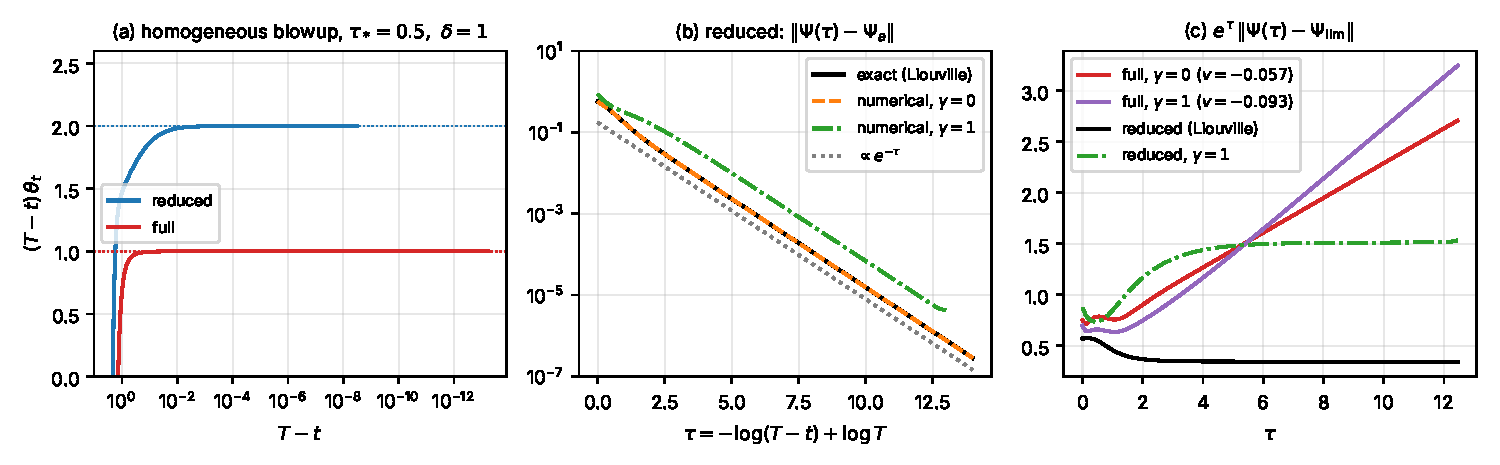
\includegraphics[width=\textwidth]{figures/therm_blowup.pdf}
\caption{(a) Homogeneous blowup of \cref{therm:eq:full,therm:eq:reduced} with
$\varepsilon=0$, $\tau_*=0.5$, $\delta=1$, $\theta(0)=\theta'(0)=0$: $(T-t)\theta_t\to2$ for the reduced and $\to1$
for the full model.  (b) Reduced model, $d=1$: distance to the boosted profile in similarity
variables, exact Liouville solution vs.\ numerics ($\gamma=0$), and the damped case
$\gamma=1$; all decay like $e^{-\tau}$ (gap $1$, sharp).  (c) $e^{\tau}\times$distance to the
limiting profile: constant for the reduced model ($\gamma=0,1$), linear growth ($\tau e^{-\tau}$
decay, Jordan block at $\lambda=-1$) for the full model \cref{therm:eq:fullN}
($\gamma=0,1$; $v$ = fitted tilt).  Code: \texttt{code/therm\_sim1d.py}.}
\label{therm:fig:blowup}
\end{figure}

% ---------------------------------------------------------------------------
\subsection{Arrhenius kinetics: no blowup}
\label{therm:sec:arrhenius}

For $\varepsilon>0$, $f_\varepsilon(\theta)=\delta\exp(\theta/(1+\varepsilon\theta))$ on $\theta>-1/\varepsilon$ (absolute temperature
positive) satisfies $0<f_\varepsilon\le\delta e^{1/\varepsilon}$, and $f_\varepsilon$ together with all derivatives
tends to $0$ as $\theta\downarrow-1/\varepsilon$; hence $f_\varepsilon$ extends by $0$ to a $C^\infty$, bounded,
globally Lipschitz function on $\mathbb{R}$ (hyperbolic models have no maximum principle,
so this extension matters).  Then \cref{therm:eq:reduced} is a semilinear wave
equation with globally Lipschitz nonlinearity, and \cref{therm:eq:full} has in
addition the term $\tau_* f_\varepsilon'(\theta)\theta_t$, linear in $\theta_t$ with a bounded (possibly
anti-damping) coefficient.  Standard energy estimates give global smooth
solutions growing at most exponentially: \emph{there is no finite-time blowup}.
Thermal ``explosion'' is a rapid transition to $\theta=O(1/\varepsilon)$ (temperature rise
of order $\Theta_0$; reactant consumption, neglected here, limits it further).  The FK
blowup is an \emph{intermediate asymptotic} regime, valid while $\varepsilon\theta\ll1$: in
similarity time up to $\tau_{\max}\approx1/(2\varepsilon)$ (reduced) or $\tau_{\max}\approx1/\varepsilon$ (full).  For
typical activation energies $E/(R\Theta_0)=1/\varepsilon\approx20$--$40$ this window spans many
$e$-folds, so the convergence rates above are physically meaningful.

% ---------------------------------------------------------------------------
\subsection{Status, literature and caveats}
\label{therm:sec:status}

\begin{table}[t]
\centering
\small
\begin{tabular}{@{}p{0.31\textwidth}p{0.33\textwidth}p{0.29\textwidth}@{}}
\toprule
Known & Derived here (proof sketch) & Numerical / conjectural\\
\midrule
Liouville's formula \cite{Liouville1853}; MCV law and both model forms
\cite{Cattaneo1958,MendezFortFarjas1999}; for $\square u=e^u$: blowup on a
surface with logarithmic behaviour for data near constants, any $d$
\cite{Kichenassamy1996}; $1$D blowup curves and rates
\cite{Godin2000,Godin2001,AzaiezMasmoudiZaag2016}; Donninger machinery for powers
\cite{DonningerSchoerkhuber2012,DonningerSchoerkhuber2014,DonningerSchoerkhuber2017,Ostermann2024}.
&
Spectra \cref{therm:eq:eigs,therm:eq:eigsfull} with all integer/log cases;
semisimplicity; Jordan block (full); free rates; \cref{therm:thm:reduced}
and \cref{therm:rem:damping}; exact $1$D structure
(\cref{therm:prop:liouville,therm:cor:liouville}); homogeneous dynamics of the full
model; tilted family; \cref{therm:thm:full} (less checked); Arrhenius global existence.
&
$1$D simulations of both models (rates, tilt $=$ slope); exact essential
growth bound $\frac{d+1}2-k$ for the full model; non-ODE (non-homogeneous)
self-similar profiles were not searched for.\\
\bottomrule
\end{tabular}
\caption{Status of the results of \cref{therm:sec}.}
\label{therm:tab:status}
\end{table}

\paragraph{Novelty.}  For the method in general see the survey \cite{Donninger2024}.
We did not find a Donninger-type (similarity variables,
$H^k$, spectral) stability theorem for $u_{tt}-\Delta u=e^u$, nor any analysis of the
MCV-consistent equation with the $\partial_t(e^u)$ nonlinearity.  However,
Kichenassamy's result \cite{Kichenassamy1996} (Fuchsian reduction and Nash--Moser,
data near constants, i.e.\ near the ODE blowup) already implies stability of the
ODE blowup for $\square u=e^u$ in a high-regularity sense, including the
logarithmic terms (absent iff the blowup surface has vanishing scalar
curvature); we have only seen the abstract of \cite{Kichenassamy1996}.
\Cref{therm:thm:reduced} should therefore be viewed as a routine but
quantitative adaptation ($H^k$, $k>d/2$, explicit rate $(T-t)^\omega$, data only on a
ball), while the full Cattaneo model (\cref{therm:sec:full}) appears to be new.
The literature search was limited (search budget), so this assessment is
provisional.

\paragraph{Caveats.}  (1) \Cref{therm:thm:reduced,therm:thm:full} are proof
sketches; the uniform semigroup bounds on the stable subspace (beyond the
quasi-compactness of \cref{therm:lem:free}) and the modulation in $(T,a)$ are
adapted from the power case without writing out all details.
(2) For the full model only the crude essential bound $\frac d2+1-k$ is proved.
(3) Damping requires $\gamma T$ small, reached by Cauchy stability.  (4) The
analysis is local in a light cone; boundary conditions, the Gelfand threshold
$\delta_{\rm crit}$ of bounded domains, and whether blowup occurs at all for given
data are not addressed.  (5) Results concern the FK limit $\varepsilon=0$;
with Arrhenius kinetics there is no blowup (\cref{therm:sec:arrhenius}).

\section{The power family, Klein--Gordon and lower-order perturbations}
\label{power:sec}

This section (i) puts softening ``Duffing continua'', the focusing
Klein--Gordon ($\phi^4$) equation and MEMS touchdown into one family
$\partial_t^2u-\Delta u=F_p(u)$, $p\notin[-1,1]$, and proves the spectral
theorem for its ODE blowup in all angular sectors (a detailed version of
\cref{fw:thm-spec}, including the integer, logarithmic and Jordan cases);
(ii) compares it with the published results; (iii) treats damping and
restoring forces $\gamma\partial_tu+m^2u$, which destroy exact self-similarity,
via an ``asymptotically autonomous'' lemma (\cref{power:lem-lower-order}) that
the model sections can cite. Labels: \textbf{(K)} known (with reference),
\textbf{(P)} proved here, \textbf{(S)} sketched here, \textbf{(N)} numerical or
conjectural. Symbolic claims are checked in \texttt{code/power\_symbolic.py},
numerical ones in \texttt{code/power\_spectrum.py}.

\subsection{Industrial models and the unified family}
\label{power:subsec-models}

\paragraph{Duffing continua.} A string ($d=1$) or membrane ($d=2$) with density
$\varrho$, tension $\mathcal T$, viscous damping $c_v$, on a nonlinear Winkler
foundation with restoring force $k_1u-k_3u^3$ per unit area obeys
\begin{equation}\label{power:eq-duffing}
  \varrho\,\partial_t^2u+c_v\,\partial_tu-\mathcal T\Delta u+k_1u=k_3u^3 .
\end{equation}
For a \emph{softening} foundation ($k_3>0$; continuum version of the softening
Duffing oscillator \cite{NayfehMook1979,KovacicBrennan2011}) the potential
$\frac12k_1u^2-\frac14k_3u^4$ has a barrier at $u_b=(k_1/k_3)^{1/2}$, and
homogeneous motions above it escape in finite time. With $t=t_*t'$,
$x=(\mathcal T/\varrho)^{1/2}t_*x'$, $u=(\varrho/(k_3t_*^2))^{1/2}u'$ (primes dropped),
\begin{equation}\label{power:eq-nlkg}
  \partial_t^2u+\gamma\,\partial_tu+m^2u-\Delta u=u^3,\qquad
  \gamma=c_vt_*/\varrho,\quad m^2=k_1t_*^2/\varrho .
\end{equation}
Taking $t_*$ equal to the blowup time shows that $\gamma$, $m$ measure the
damping time and foundation period \emph{relative to the blowup time}. For
$\gamma=0$ this is the focusing cubic Klein--Gordon ($\phi^4$) equation.
Physical caveats: the cubic law is a truncation, so ``blowup'' means dynamic
escape (snap-through) and the self-similar profile describes the escaping
region only while the foundation law is valid; Euler--Bernoulli beams
($\partial_x^4$ instead of $-\Delta$) are not covered.

\paragraph{The unified family.} For $p\in\mathbb R\setminus[-1,1]$ let
\begin{equation}\label{power:eq-family}
  \partial_t^2u-\Delta u=F_p(u):=\operatorname{sgn}(p-1)\,|u|^{p-1}u,\qquad
  s:=\tfrac{2}{p-1}\in(-1,0)\cup(0,\infty).
\end{equation}
For $p>1$ this is the focusing power equation; for $p=-q<-1$ and $u=w>0$ it is
the MEMS equation $\partial_t^2w-\Delta w=-w^{-q}$ for the gap $w$ ($\lambda$ in
$-\lambda w^{-q}$ scales out), with $s=-\sigma=-\frac{2}{q+1}$ as in
\cref{mems:sec}. The sign makes the force point \emph{towards} the singularity
($u\to\infty$, resp.\ $w\to0$). The critical Sobolev exponent is
$s_c=\frac d2-s$. See \cref{power:tab-models}.

\begin{table}[ht]
\centering\small
\begin{tabular}{@{}lcccc@{}}
\toprule
model & $p$ & $s$ & $V_0=(s+1)(s+2)$ & $\omega_0=\min\{1,2s+2\}$\\
\midrule
softening string/membrane, $\phi^4$ & $3$ & $1$ & $6$ & $1$\\
focusing NLKG/NLW & $p>1$ & $\frac{2}{p-1}$ & $\frac{2p(p+1)}{(p-1)^2}$ & $1$\\
MEMS, general & $-q<-1$ & $-\frac{2}{q+1}$ & $\frac{2q(q-1)}{(q+1)^2}$ & $\min\{1,\frac{2(q-1)}{q+1}\}$\\
MEMS, parallel plate & $-2$ & $-\frac23$ & $\frac49$ & $\frac23$\\
\bottomrule
\end{tabular}
\caption{The unified family \eqref{power:eq-family}; $\omega_0$ is the spectral
gap of \cref{power:cor-gap}.}
\label{power:tab-models}
\end{table}

\subsection{ODE blowup and the excluded range \texorpdfstring{$-1\le p\le1$}{-1<=p<=1}}
\label{power:subsec-ode}

\begin{proposition}[ODE profile; \textbf{(P)}]\label{power:prop-ode}
Let $p\neq\pm1$, $s=\frac2{p-1}$. Then $u''=F_p(u)$ has a solution
$u_T=\kappa(T-t)^{-s}$, $\kappa>0$, iff $p\notin[-1,1]$, and then
\[
  \kappa^{p-1}=\operatorname{sgn}(p-1)\,s(s+1)=|s(s+1)|,\qquad
  V_0:=F_p'(u_T)(T-t)^2=p\,s(s+1)=(s+1)(s+2).
\]
For MEMS with general $\lambda$: $\kappa^{q+1}=\lambda/(\sigma(1-\sigma))$,
$V_0=\lambda q\kappa^{-q-1}=q\sigma(1-\sigma)=(1-\sigma)(2-\sigma)>0$ (note
$F'(w)=+\lambda qw^{-q-1}$).
\end{proposition}
\begin{proof}
$u_T''=s(s+1)\kappa(T-t)^{-s-2}$, $F_p(u_T)=\operatorname{sgn}(p-1)\kappa^p(T-t)^{-sp}$
and $sp=s+2$. For $s>0$ and $s\in(-1,0)$ the product $\operatorname{sgn}(p-1)s(s+1)$
is positive; for $p\in(-1,1)$, $s<-1$ and it is negative. Euler's relation
$uF_p'(u)=pF_p(u)$ gives $V_0=p\,s(s+1)$, and $ps=s+2$.
\end{proof}

\begin{remark}[Why $-1\le p\le1$ is excluded; \textbf{(P)}]\label{power:rem-small-p}
For $p\in(-1,1)$ a self-similar solution would have $s<-1$, so $u_T$
\emph{and} $\partial_tu_T$ tend to $0$: no singularity of $(u,\partial_tu)$; even
with the opposite sign (where $\kappa$ exists) it is non-generic, the
second eigenvalue family below starting at $-2s-2>0$. For the MEMS sign and
$0<q<1$ the gap closes with finite speed, $w\approx\sqrt{2E}(T-t)$, and for $q=1$
with a logarithmic correction, $w\approx(T-t)\sqrt{2|\log(T-t)|}$ (from
$\frac12w'^2+\log w=E$). Self-similar ODE blowup thus exists exactly for
$s\in(-1,0)\cup(0,\infty)$, which is also where $\omega_0>0$.
\end{remark}

\paragraph{Symmetries.} Besides $T$, the boosted profiles \eqref{fw:boost}
$u_{T,a}=\kappa(1-|a|^2)^{s/2}(T-t+a\cdot x)^{-s}$, $|a|<1$, blow up on the
spacelike hyperplane $\{t=T+a\cdot x\}$ and are stationary in similarity
variables, $\psi_a(\xi)=\kappa(1-|a|^2)^{s/2}(1+a\cdot\xi)^{-s}$; this holds verbatim
in the MEMS range. Space translations act trivially on $u_T$.

\subsection{The linearised operator and the free flow}
\label{power:subsec-linear}

With $\Psi=\Psi_*+\Phi$, $\Psi_*=(\kappa,s\kappa)$ in \eqref{fw:system},
$\partial_\tau\Phi=\mathbf L\Phi+\mathbf N(\Phi)$ on
$\mathcal H^k=H^k(B^d)\times H^{k-1}(B^d)$, where
\[
  \mathbf L\Phi=\begin{pmatrix}-\Lambda\phi_1-s\phi_1+\phi_2\\ \Delta\phi_1-\Lambda\phi_2-(s+1)\phi_2+V_0\phi_1\end{pmatrix},\quad
  \mathbf N(\Phi)=\begin{pmatrix}0\\ F_p(\kappa+\phi_1)-F_p(\kappa)-V_0\phi_1\end{pmatrix}.
\]
Since $\kappa>0$, $F_p$ is real analytic near $\kappa$ for every real $p$
(non-integer $p$ and the singular MEMS force included); for $k>\frac d2$ and
$\|\phi_1\|_{L^\infty}\le\kappa/2$, $\mathbf N$ is locally Lipschitz with a
quadratic bound. No regularity restriction on $p$ arises.

\begin{lemma}[Polynomial invariance; \textbf{(P)}]\label{power:lem-poly}
Let $\mathcal P_N$ be the polynomials of degree $\le N$ in $\xi$. Then $\mathbf L$
maps $\mathcal P_N^2$ into itself and acts on homogeneous parts of degree $j$
(modulo $\mathcal P_{j-1}^2$) as
$M_j=\bigl(\begin{smallmatrix}-s-j&1\\ V_0&-s-1-j\end{smallmatrix}\bigr)$, with
eigenvalues $1-j$ and $-2s-2-j$. For $V_0=0$ (the free operator $\mathbf L_0$)
they are $-s-j$, $-s-1-j$; in particular $\mathbf L_0(1,0)=-s(1,0)$. On
constants $\mathbf L$ has the eigenvalues $1$ (time translation) and $-2s-2$.
\end{lemma}
\begin{proof}
$\Lambda$ multiplies homogeneous polynomials of degree $j$ by $j$, $\Delta$
lowers the degree by two, and $\det(M_j-\mu)=(\mu+j-1)(\mu+j+2s+2)$ since
$V_0=(s+1)(s+2)$.
\end{proof}

So every eigenvalue of \cref{power:thm-spectrum} with a polynomial
eigenfunction is visible algebraically; the content of the theorem is that
there are no others. Note also that polynomial (collocation, Galerkin)
discretisations of $\mathbf L$ are \emph{exact} on $\mathcal P_N^2$ and cannot detect
non-polynomial eigenfunctions (\cref{power:subsec-numerics}).

\begin{lemma}[Free flow; (a) \textbf{(P)}, (b) \textbf{(S)}]\label{power:lem-free}
Let $\omega_k:=k-s_c=k-\frac d2+s$. (a) $-s$ is an eigenvalue of $\mathbf L_0$ on
every $\mathcal H^k$ (eigenfunction $(1,0)$, i.e.\ $u\equiv$ const), so the growth
bound of $e^{\tau\mathbf L_0}$ is $\ge-s$; in the MEMS range $-s=\sigma>0$ and the
free flow grows. (b) $\mathbf L_0=\tilde{\mathbf L}_0+\mathbf K$ with $\mathbf K$ of finite
rank and $\|e^{\tau\tilde{\mathbf L}_0}\|\le Me^{-\omega_k\tau}$. Hence, if $\omega_k>0$,
$\sigma(\mathbf L)\cap\{\operatorname{Re}\lambda>-\omega_k\}$ consists of isolated
eigenvalues of finite algebraic multiplicity.
\end{lemma}
\begin{proof}[Proof of (b), sketch]
For $|\beta|=k-1$ let $f=\partial^\beta\phi_1$, $g=\partial^\beta\phi_2$. Since
$\partial^\beta\Lambda=(\Lambda+k-1)\partial^\beta$, the free flow gives
$\partial_\tau f=-(\Lambda+s+k-1)f+g$, $\partial_\tau g=\Delta f-(\Lambda+s+k)g$, and
with $\int_B h\Lambda h=-\frac d2\int_Bh^2+\frac12\int_{\partial B}h^2$,
\begin{multline*}
  \tfrac12\tfrac{d}{d\tau}\bigl(\|\nabla f\|^2+\|g\|^2\bigr)
  =-\omega_k\bigl(\|\nabla f\|^2+\|g\|^2\bigr)\\
  -\tfrac12\int_{\partial B}\bigl(|\nabla f|^2-(\partial_rf)^2+(\partial_rf-g)^2\bigr)
  \le-\omega_k\bigl(\|\nabla f\|^2+\|g\|^2\bigr),
\end{multline*}
the boundary term having a sign because $\partial B$ is the light cone. So the
seminorm
\[
  E_k(\Phi)=\textstyle\sum_{|\beta|=k-1}\bigl(\|\nabla\partial^\beta\phi_1\|^2+\|\partial^\beta\phi_2\|^2\bigr)
\]
decays at rate $2\omega_k$. Its kernel $\mathcal P_{k-1}\times\mathcal P_{k-2}$ is
finite-dimensional and $\mathbf L_0$-invariant (\cref{power:lem-poly}), and
$E_k^{1/2}$ is equivalent to the quotient norm (Bramble--Hilbert), so $\mathbf L_0$
is block-triangular with a quotient block of growth bound $\le-\omega_k$ and a
finite-rank remainder. $\mathbf L'=(0,V_0\phi_1)$ is compact, and the rest is
\cite[Ch.~IV]{EngelNagel2000}. Rigorous inner products of this type are
constructed in \cite{Ostermann2024,Glogic2025}.
\end{proof}

\begin{remark}[Regularity threshold; the Lumer--Phillips step]\label{power:rem-LP}
The free decay rate is $\omega_k=k-s_c$, so exponential decay needs regularity
strictly above scaling, $k>s_c$; at $k=s_c$ one needs Strichartz estimates in
similarity coordinates \cite{Donninger2017,DonningerRao2018,Wallauch2022}. To
see the full gap one needs $k>s_c+\omega_0$; for MEMS $k>\frac d2+\sigma+\omega_0$
(e.g.\ $q=2$: $k\ge2$ for $d=1$, $k\ge3$ for $d=2$). The simplest
Lumer--Phillips argument, an inner product in which $\mathbf L_0$ itself is
dissipative with bound $-s$, is sharp by (a) and yields the rate
$\min\{1,s\}$; we believe this is the origin of the exponent $\min\{1,s_p\}$ in
\cite{Ostermann2024}. In the MEMS range it yields nothing ($-s=\sigma>0$; no
inner product makes $\mathbf L_0$ dissipative with negative bound), and the
splitting (b) is necessary. The finite-rank part is absorbed into the compact
perturbation, so the positive free eigenvalue $\sigma$ is harmless: it is not an
eigenvalue of $\mathbf L$.
\end{remark}

\subsection{The spectral theorem in all angular sectors}
\label{power:subsec-spectrum}

Let $\mathcal Y_\ell$ be the spherical harmonics of degree $\ell$ ($d\ge2$); for
$d=1$, $\mathcal Y_0=\{1\}$, $\mathcal Y_1=\{\operatorname{sgn}\xi\}$, $\mathcal Y_{\ell\ge2}=\{0\}$.

\begin{theorem}[Spectrum of the ODE blowup; \textbf{(P)}]\label{power:thm-spectrum}
Let $d\ge1$, $p\in\mathbb R\setminus[-1,1]$, $k\in\mathbb N$, $\omega_k>0$, and
$\operatorname{Re}\lambda>-\omega_k$. Then $\lambda$ is an eigenvalue of $\mathbf L$ on
$\mathcal H^k$ iff
\[
  \lambda\in\Sigma_s:=\{1-\ell-2n\}\cup\{-2s-2-\ell-2n\},\qquad n\in\mathbb N_0,\ \mathcal Y_\ell\neq\{0\}.
\]
In the sector $\ell$ the eigenfunctions are $(g,(\lambda+s+\Lambda)g)$,
$g=|\xi|^\ell Y_\ell\,{}_2F_1(\alpha,\beta;\frac d2+\ell;|\xi|^2)$, $Y_\ell\in\mathcal Y_\ell$,
$\alpha=\frac{\lambda+\ell-1}{2}$, $\beta=\frac{\lambda+\ell+2s+2}{2}$ (a polynomial of
degree $n$ in $|\xi|^2$). All eigenvalues are real, and:
\begin{enumerate}[nosep,label=(\alph*)]
\item $\lambda=1$ occurs only for $\ell=0$, with $\Phi=(1,s+1)=$ time-translation mode;
\item $\lambda=0$ occurs only for $\ell=1$, with $\Phi=(\xi_j,(s+1)\xi_j)$,
  $j=1,\dots,d$, the boost modes $\propto\partial_{a_j}\Psi_a|_{a=0}$;
\item both are semisimple. The two families collide iff $s\in\frac12+\mathbb Z$
  ($p\in\{5,\frac73,\frac95,\dots\}$ or $q=3$); at the lowest collisions
  ($s=-\frac12,\lambda=-1$; $s=\frac12,\lambda=-3$; $\ell=0$) there is a Jordan block of
  length two.
\end{enumerate}
\end{theorem}

\begin{proof}
\emph{Reduction.} An eigenfunction has $\phi_2=(\lambda+s+\Lambda)\phi_1$, and
$g=\phi_1$ solves \eqref{fw:eig} with $a=s+\lambda$, which is elliptic in the open
ball; so $g\in C^\infty(B^d)$. Each spherical-harmonic component
$|\xi|^\ell Y_\ell h(|\xi|^2)$ is again an $H^k$ solution, and $h$ solves
\eqref{fw:hyp} with $c=\frac d2+\ell$, $\alpha+\beta+1=a+\ell+\frac32$,
$\alpha\beta=\frac14[(a+\ell)(a+\ell+1)-V_0]$; with $a_1=s+1$, $a_2=-(s+2)$ this
gives the stated $\alpha,\beta$. (The sector $\ell$ in dimension $d$ is the radial
problem in dimension $d+2\ell$ with $\lambda\mapsto\lambda+\ell$.)
\emph{At $z=0$} the second Frobenius solution gives $|\xi|^{2-d-\ell}Y_\ell$ (or
$\log|\xi|$, or $|\xi|$, $\operatorname{sgn}\xi$ for $d\le2$), which is not smooth; so
$h\propto{}_2F_1(\alpha,\beta;c;z)$.
\emph{At $z=1$} the exponents are $0$ and $\mu=\frac{d-1}{2}-s-\lambda$; the non-analytic
local solutions behave like $(1-|\xi|^2)^\mu$, $(1-|\xi|^2)^m\log(1-|\xi|^2)$ ($\mu=m\in\mathbb
N_0$) or $(1-|\xi|^2)^{-m}$ ($\mu=-m<0$), and lie in $H^k$ near $\partial B$ only if
$\operatorname{Re}\mu>k-\frac12$, i.e.\ $\operatorname{Re}\lambda<-\omega_k$. Hence, for
$\operatorname{Re}\lambda>-\omega_k$, $h$ is an eigenfunction iff it is analytic at $z=1$.
\emph{Monodromy.} The hypergeometric equation is Fuchsian with singular points
$0,1,\infty$. A solution analytic at $0$ and at $1$ has trivial monodromy and
extends to an entire function of polynomial growth (as $\infty$ is regular
singular), i.e.\ a polynomial; and ${}_2F_1(\alpha,\beta;c;z)$ is a polynomial iff
$\alpha\in-\mathbb N_0$ or $\beta\in-\mathbb N_0$. This handles the integer and logarithmic
cases uniformly (alternatively use the connection formulae
\cite[\S15.8]{OlverEtAl2010}). $\alpha=-n$ gives $\lambda=1-\ell-2n$, $\beta=-n$ gives
$\lambda=-2s-2-\ell-2n$.
\emph{(a), (b)}: $1-\ell-2n\ge0$ iff $(\ell,n)\in\{(0,0),(1,0)\}$, and
$-2s-2-\ell-2n<0$ for $s>-1$.
\emph{(c)}: a generalised eigenvector solves $(\mathbf L-\lambda)\Phi=\Phi_\lambda$;
eliminating $\phi_2$ gives an inhomogeneous hypergeometric equation with
polynomial right-hand side, so by the same monodromy argument an $\mathcal H^k$
solution is a polynomial. By \cref{power:lem-poly} its degree is at most
$\max\{\deg\Phi_\lambda,j_*\}$, where $M_{j_*}-\lambda$ is singular, and the
degree-$j_*$ block requires the top part of $\Phi_\lambda$ to lie in
$\operatorname{ran}(M_{j_*}-\lambda)$. For $\lambda=1$ ($j_*=0$) and $\lambda=0$ ($j_*=1$) this
fails, as $\lambda$ is a simple eigenvalue of $M_{j_*}$ for $s>-1$. At a collision
both $\alpha,\beta\in-\mathbb N_0$ and the eigenfunction is shared by the two families
(e.g.\ $s=-\frac12$, $\lambda=-1$: $g\equiv1$), and a generalised eigenvector exists:
$(\mathbf L+1)\Phi=(1,-\frac32)$ with $\phi_1=-|\xi|^2/3$ ($d=3$), and for $s=\frac12$,
$\lambda=-3$, $(\mathbf L+3)\Phi=(1,-\frac52)$ with $\phi_1=-\frac23|\xi|^2+\frac2{15}|\xi|^4$ ($d=3$). That all non-colliding eigenvalues
are semisimple, and all collisions give Jordan blocks (a double zero of
$1/(\Gamma(\alpha)\Gamma(\beta))$), is expected but only checked in these cases
\textbf{(S)}.
\end{proof}

\begin{corollary}[Spectral gap; \textbf{(P)}]\label{power:cor-gap}
If $\omega_k>\omega_0$, then
$\sup\{\operatorname{Re}\lambda:\lambda\in\sigma(\mathbf L)\setminus\{0,1\}\}=-\omega_0$,
\[
  \omega_0=\min\{1,2s+2\}=\begin{cases}1,& p>1\text{ or }p=-q,\ q\ge3,\\[2pt]
  \frac{2(q-1)}{q+1},& p=-q,\ 1<q\le3.\end{cases}
\]
The gap eigenvalue is $-1$ ($\ell=0,n=1$ and $\ell=2,n=0$) for $p>1$, $q\ge3$, and
the spatially homogeneous mode $-2s-2=-2(1-\sigma)$ for $q<3$; at $q=3$ they form a
Jordan block. For the parallel-plate force $q=2$: $\omega_0=\frac23$.
\end{corollary}

\subsection{What is proved in the literature}
\label{power:subsec-lit}

All results below concern $p>1$; for the MEMS range see \cref{mems:sec}.
\textbf{(K)}:
% TODO verify: range 1<p<=3 in DS2012; data space/range in DS2017; rate in Ostermann Thm 1.1;
% content of MerleZaag2016 (full texts not accessed, see "Source check" below)
\cite{DonningerSchoerkhuber2012}: $d=3$, radial, $1<p\le3$, stability of $u_T$ in
the energy topology (complementing \cite{MerleZaag2003,MerleZaag2007}); here
$k=1$ and $\omega_1=s-\frac12\ge\frac12$, consistent with \cref{power:rem-LP}.
\cite{DonningerSchoerkhuber2014}: $d=3$, radial, $p>3$, an open set of radial data
above energy regularity blows up via $u_T$.
\cite{DonningerSchoerkhuber2016}: $d=3$, energy supercritical, \emph{no symmetry
assumption}. \cite{DonningerSchoerkhuber2017}: radial data in odd $d\ge5$,
energy-supercritical powers, data in $H^{(d+1)/2}\times H^{(d-1)/2}$.
\cite{Ostermann2024}: all $d\ge1$, all $p>1$, no symmetry; data in
$H^k\times H^{k-1}$, $k>\frac d2$; convergence to a Lorentz-boosted ODE profile with
parameters $(T^*,\beta^*)$, with decay exponent governed by $\min\{1,s_p\}$;
dissipative inner products on $H^k$ for all $d$ and integer $k$.
\cite{Liu2025}: superconformal powers, all dimensions, mode stability via Lorentz
transformations and asymptotic stability of the ODE blowup family, extending
\cite{MerleZaag2016} (subconformal, energy space, explicit Lorentz family, no
symmetry) and \cite{Ostermann2024}. Critical case $d=3$, $p=5$:
\cite{Donninger2017,DonningerRao2018}; cubic in higher dimensions:
\cite{ChatzikaleasDonninger2019}.

\emph{Cross-check.} In all these works the only non-negative eigenvalues are
$\lambda=1$ and, nonradially, $\lambda=0$, as in \cref{power:thm-spectrum}. The
exponent $\min\{1,s_p\}$ of \cite{Ostermann2024} equals the gap $\omega_0=1$ for
$p\le3$ but is smaller for $p>3$; it reflects the free eigenvalue $-s$ of
constants (\cref{power:rem-LP}), not an eigenvalue of $\mathbf L$ (the second
family starts at $-2s-2<-s$). With \cref{power:lem-free}(b) the rate should
improve to $\min\{1,\omega_k\}-\varepsilon$, i.e.\ $1-\varepsilon$ for $k$ large
\textbf{(S)}. \emph{Source check:} the full texts could not be accessed here;
the statements are taken from abstracts/indexing data and
\texttt{bib/lit.bib}, and the details (ranges of $p$, spaces, rates) should be
checked against the papers.

\subsection{Lower-order perturbations: damping and restoring forces}
\label{power:subsec-lower}

Consider, with $\gamma,m^2\in\mathbb R$,
\begin{equation}\label{power:eq-pert}
  \partial_t^2u+\gamma\,\partial_tu+m^2u-\Delta u=F_p(u).
\end{equation}
With $T-t=Te^{-\tau}$ and \eqref{fw:psi} one obtains \emph{exactly}
(\textbf{(P)}, symbolic identity)
\begin{equation}\label{power:eq-sim-pert}
  \partial_\tau\Psi=\mathbf L_0\Psi+\begin{pmatrix}0\\F_p(\psi_1)\end{pmatrix}
  -\begin{pmatrix}0\\ \gamma Te^{-\tau}\psi_2+m^2T^2e^{-2\tau}\psi_1\end{pmatrix}:
\end{equation}
non-autonomous terms of size $e^{-\tau}$ (damping) and $e^{-2\tau}$ (mass), with $T$
in the coefficients.

\begin{proposition}[Perturbed ODE blowup; expansion \textbf{(P)}, existence
\textbf{(S)}]\label{power:prop-ode-pert}
As $\rho=T-t\downarrow0$, spatially homogeneous solutions of \eqref{power:eq-pert}
blowing up at $T$ form a one-parameter family,
\begin{gather*}
  U_T=\kappa\rho^{-s}\bigl(1+a_1\rho+a_2\rho^2+\dots\bigr)+c\,\rho^{s+2}(1+\dots),\\
  a_1=\frac{\gamma s}{2(2s+1)},\qquad
  a_2=\frac{\gamma^2(3s^2-5s-4)}{24(2s+1)^2}+\frac{m^2}{6s}.
\end{gather*}
The order-$j$ coefficient obeys $-(j+1)(2s+2-j)a_j=$ (lower orders); the indicial
roots $j=-1$, $j=2s+2$ are the eigenvalues $1$, $-2s-2$ of \cref{power:lem-poly}. If
$2s+2\in\mathbb N$ and compatibility fails, $\rho^{2s+2}\log\rho$ terms appear: for
$p=3$ iff $\gamma^2(9m^2-2\gamma^2)\neq0$ (cf.\ the Painlevé condition $m^2=2\gamma^2/9$
for the damped Duffing equation), for $p=5$ iff $\gamma(16m^2-3\gamma^2)\neq0$, and
for MEMS $q=3$ at first order whenever $\gamma\ne0$:
$U_T=\sqrt2\rho^{1/2}(1+\frac\gamma4\rho\log\rho+c\rho+\dots)$. Hence
$\Psi_T(\tau)-\Psi_*=O(e^{-\tau})$ if $\gamma\neq0$ ($O(\tau e^{-\tau})$ for $q=3$) and
$O(e^{-2\tau})$ if $\gamma=0$.
\end{proposition}

\begin{lemma}[The tilted family survives damping; \textbf{(P)}]\label{power:lem-tilt}
For $|a|<1$, $u=W(T-t+a\cdot x)$ solves \eqref{power:eq-pert} iff
$(1-|a|^2)W''-\gamma W'+m^2W=F_p(W)$. Hence
$u_{T,a}(t,x):=U^{\gamma_a}\bigl((T-t+a\cdot x)/\sqrt{1-|a|^2}\bigr)$, with $U^{\gamma_a}(\rho)$ the
perturbed ODE blowup of \cref{power:prop-ode-pert} for damping
$\gamma_a=\gamma/\sqrt{1-|a|^2}$, is an exact solution blowing up on
$\{t=T+a\cdot x\}$, and $\Psi_{T,a}(\tau)=\Psi_a+O(e^{-\tau})$.
\end{lemma}
\begin{proof}
$\partial_t^2u=W''$, $\Delta u=|a|^2W''$, $\partial_tu=-W'$; then rescale the
argument of $W$ by $\sqrt{1-|a|^2}$.
\end{proof}

Thus the mass preserves Lorentz invariance (for $\gamma=0$ the $u_{T,a}$ are
boosts of $U_T$) and damping breaks it, but the $d$-parameter tilted family
remains an exact family of solutions for every $\gamma$; only translation
invariance in $(t,x)$ is used. The neutral modes $\lambda=0$ are therefore still
generated by exact solutions, and no dynamical modulation of the boost
parameter (as anticipated in \cref{fw:subsec-lower}) is needed.

\begin{lemma}[Asymptotically autonomous Lyapunov--Perron lemma; \textbf{(S)}]
\label{power:lem-lower-order}
Let $\mathbf L$ generate a $C_0$-semigroup $\mathbf S$ on a Hilbert space $\mathcal H$,
$\mathbf P=\mathbf P_1+\mathbf P_0$ a finite-rank projection commuting with $\mathbf S$,
$\mathbf L\mathbf P_1=\mathbf P_1$, $\mathbf L\mathbf P_0=0$, and
$\|\mathbf S(\tau)(\mathbf I-\mathbf P)\|\le Me^{-\bar\omega\tau}$ for some $\bar\omega\in(0,1]$. For
$\theta$ in a closed ball $\overline B\subset\mathbb R^{\operatorname{rank}\mathbf P}$ let
$\mathbf B_\theta(\tau)\in\mathcal B(\mathcal H)$ be strongly continuous with
$\sup_\tau\|\mathbf B_\theta(\tau)\|\le\beta$ (in applications
$\mathbf B_\theta(\tau)=O(|a|)+O(e^{-\tau})$), and $\mathbf N_\theta(\tau,\cdot)$ with
$\mathbf N_\theta(\tau,0)=0$,
$\|\mathbf N_\theta(\tau,\Phi)-\mathbf N_\theta(\tau,\tilde\Phi)\|\le C_N(\|\Phi\|+\|\tilde\Phi\|)\|\Phi-\tilde\Phi\|$
for $\|\Phi\|,\|\tilde\Phi\|\le1$, all continuous in $\theta$. Consider
\begin{equation}\label{power:eq-abstract}
  \partial_\tau\Phi=\mathbf L\Phi+\mathbf B_\theta(\tau)\Phi+\mathbf N_\theta(\tau,\Phi),\qquad\Phi(0)=\mathbf u_\theta .
\end{equation}
For every $\omega\in(0,\bar\omega)$ there are $\beta_0,\delta_0,C>0$ such that if $\beta\le\beta_0$ and
$\|\mathbf u_\theta\|\le\delta\le\delta_0$:
\begin{enumerate}[nosep,label=(\roman*)]
\item there is a unique $\Phi_\theta$ with $\sup_\tau e^{\omega\tau}\|\Phi_\theta(\tau)\|\le
  C\delta$ solving
  $\Phi(\tau)=\mathbf S(\tau)[\mathbf u_\theta-\mathbf C_\theta(\Phi)]+\int_0^\tau\mathbf S(\tau-\sigma)\mathbf G_\theta(\sigma)\,d\sigma$,
  where $\mathbf G_\theta=\mathbf B_\theta\Phi+\mathbf N_\theta(\sigma,\Phi)$ and
  $\mathbf C_\theta(\Phi)=\mathbf P\mathbf u_\theta+\int_0^\infty(e^{-\sigma}\mathbf P_1+\mathbf P_0)\mathbf G_\theta(\sigma)\,d\sigma$;
\item $\Phi_\theta$ solves \eqref{power:eq-abstract} iff $\mathbf C_\theta(\Phi_\theta)=0$;
\item if $\theta\mapsto\mathbf P\mathbf u_\theta$ is a homeomorphism onto a neighbourhood of
  $0$ in $\operatorname{ran}\mathbf P$ with $\delta$-independent Lipschitz inverse
  (transversality), then for small $\delta$ some $\theta^*$ has
  $\mathbf C_{\theta^*}(\Phi_{\theta^*})=0$.
\end{enumerate}
An inhomogeneity $e^{-\tau}\mathbf g_\theta(\tau)$, $\|\mathbf g_\theta\|\le\delta$, may be
added; then (i)--(iii) hold for $\omega<\min\{\bar\omega,1\}$.
\end{lemma}
\begin{proof}[Sketch]
In $\mathcal X=\{\Phi:\|\Phi\|_{\mathcal X}=\sup e^{\omega\tau}\|\Phi(\tau)\|<\infty\}$,
\[
  \int_0^\tau\!Me^{-\bar\omega(\tau-\sigma)}\bigl(\beta e^{-\omega\sigma}\|\Phi\|_{\mathcal X}
  +C_Ne^{-2\omega\sigma}\|\Phi\|_{\mathcal X}^2\bigr)d\sigma
  \le Me^{-\omega\tau}\Bigl(\tfrac{\beta}{\bar\omega-\omega}\|\Phi\|_{\mathcal X}+\tfrac{C_N}{\omega}\|\Phi\|_{\mathcal X}^2\Bigr),
\]
while the corrected unstable and neutral parts
$-\int_\tau^\infty(e^{\tau-\sigma}\mathbf P_1+\mathbf P_0)\mathbf G_\theta\,d\sigma$ are
$O(\beta\omega^{-1}e^{-\omega\tau}\|\Phi\|_{\mathcal X}+C_Ne^{-2\omega\tau}\|\Phi\|_{\mathcal X}^2)$. So the map is
a contraction on a small ball if $\beta\le\beta_0$; a decay factor $e^{-\sigma}$ in
$\mathbf B_\theta$ makes the term integrable but not small, which is why the
smallness of $\beta$ (\cref{power:rem-small-beta}) is needed. A forcing is handled
by $\int_0^\tau e^{-\bar\omega(\tau-\sigma)}e^{-\sigma}d\sigma\le(1+\tau)e^{-\min\{\bar\omega,1\}\tau}$.
(ii), (iii) are as in \cite{DonningerSchoerkhuber2012,Ostermann2024} (Brouwer).
\end{proof}

\begin{remark}[Making $\beta$ small]\label{power:rem-small-beta}
Linearising \eqref{power:eq-sim-pert} at the exact family $\Psi_{T,a}(\tau)$ of
\cref{power:lem-tilt} gives \eqref{power:eq-abstract} with $\theta=(T,a)$, no
inhomogeneity, and
$\mathbf B_\theta(\tau)\Phi=\bigl(0,[F_p'(\psi_{T,a,1}(\tau))-V_0]\phi_1-\gamma Te^{-\tau}\phi_2-m^2T^2e^{-2\tau}\phi_1\bigr)$,
so $\beta\lesssim|a|+|\gamma|T+m^2T^2$. Here $|a|=O(\delta)$; to make the rest small, evolve
the data to $t_1=1-\eta$ by local well-posedness on balls (finite speed of
propagation keeps the solution $C(\eta)\varepsilon$-close to the reference on
$B_{\eta+\delta}$) and rescale by $\eta$: $(\gamma,m^2)\mapsto(\gamma\eta,m^2\eta^2)$.
\end{remark}

\begin{theorem}[ODE blowup under lower-order terms; \textbf{(S)},
conditional]\label{power:thm-lower-order}
Let $d\ge1$, $p\in\mathbb R\setminus[-1,1]$, $\gamma,m^2\in\mathbb R$, $k\in\mathbb N$,
$k>\max\{\frac d2,s_c\}$, and let $\bar\omega\in(0,1]$ be such that the autonomous estimate
$\|\mathbf S(\tau)(\mathbf I-\mathbf P)\|_{\mathcal H^k}\lesssim e^{-\bar\omega\tau}$ holds (by
\cref{power:thm-spectrum,power:lem-free} any $\bar\omega<\min\{\omega_0,\omega_k\}$; for $p>1$
and $\bar\omega<\min\{1,s\}$ this is contained in \cite{Ostermann2024}, as we read
it), and $0<\omega<\bar\omega$. Let $U$ be a spatially homogeneous solution of \eqref{power:eq-pert} on
$[0,1)$ with ODE blowup at $1$. There is $\varepsilon>0$ such that for data with
$\|(u_0,u_1)-(U(0),U'(0))\|_{H^k\times H^{k-1}(B_{1+\varepsilon})}\le\varepsilon$ there exist
$T^*$ near $1$ and small $a^*\in\mathbb R^d$ ($a^*=0$ for radial data) such that
$u$ blows up at $(T^*,0)$ and
\[
  \|\Psi(\tau)-\Psi_{T^*,a^*}(\tau)\|_{\mathcal H^k}\lesssim e^{-\omega\tau},\qquad
  \|\Psi(\tau)-\Psi_{a^*}\|_{\mathcal H^k}\lesssim e^{-\omega\tau}+e^{-\tau}
\]
($e^{-2\tau}$ instead of $e^{-\tau}$ if $\gamma=0$; $\tau e^{-\tau}$ for $q=3$,
$\gamma\neq0$). The blowup point is not a modulation parameter: any $x_0$ near $0$
may replace $0$, and then $(T^*,a^*)$ depend on $x_0$ ($a^*$ is the slope of the
blowup surface for the exact tilted solutions, and presumably to leading order
in general).
\end{theorem}
\begin{proof}[Sketch]
Reduce to small $(\gamma,m^2)$ (\cref{power:rem-small-beta}); $\mathbf N_\theta$ is
quadratic uniformly in $\tau$ because $\psi_{T,a,1}(\tau)$ stays within $\kappa/4$ of
$\psi_a$. Transversality: by \cref{power:prop-ode-pert,power:lem-tilt},
$\partial_T\Psi_{T,a}(0)$ and $\partial_{a_j}\Psi_{T,a}(0)$ are, up to nonzero factors and
errors $O(|\gamma|+m^2+|a|)$, the eigenfunctions of
\cref{power:thm-spectrum}(a),(b). Apply \cref{power:lem-lower-order}; the second
estimate follows from \cref{power:lem-tilt}.
\end{proof}

\begin{remark}[Rates and resonances]\label{power:rem-rates}
(1) Since $\omega_0\le1$ in the whole family, damping and mass never decay
\emph{slower} than the gap. If one linearises at $\Psi_a$ instead of
$\Psi_{T,a}(\tau)$, the forcing has rate $1$ (damping) or $2$ (mass); for
$\omega_0=1$ rate-$1$ forcing can resonate with the eigenvalue $-1$ and produce
$\tau e^{-\tau}$ (for $a\neq0$ the forcing has $\ell=2$ components), and at $q=3$ the
Jordan block at $-1$ does the same. Only the exponent is affected.
(2) Lower-order nonlinear terms $f$ with $|f^{(j)}(u)|\lesssim|u|^{p'-j}$ contribute
$(T-t)^{s+2}f((T-t)^{-s}\psi_1)=O(e^{-s(p-p')\tau})$; they are perturbative iff
$s(p-p')>0$ ($p'<p$ for powers, weaker singularity $q'<q$ for MEMS; a constant
load has rate $s+2$). If $s(p-p')<\omega_0$ the convergence rate drops to
$s(p-p')$ but \cref{power:lem-lower-order} still applies; this is the only way
a perturbation in this family decays more slowly than the gap.
(3) The reduction, the tilted family and the abstract lemma are elementary;
the deep input is the autonomous linear estimate, the same as in
\cite{Ostermann2024}. Local well-posedness on balls for \eqref{power:eq-pert} and the
Lipschitz dependence on $\theta$ are routine and not written out.
\end{remark}

\paragraph{Literature on the perturbed equations \textbf{(K)}.}
% TODO verify the precise classes of perturbations in Hamza--Zaag and the statements in KSV14 / DW21
Hamza and Zaag constructed Lyapunov functionals in similarity variables for
$\partial_t^2u=\Delta u+|u|^{p-1}u+f(u)+g(\partial_tu)$ with lower-order $f,g$ (including
the Klein--Gordon mass and linear damping) and proved ODE-type blowup rates:
subconformal \cite{HamzaZaag2010}, conformal \cite{HamzaZaag2012}, Klein--Gordon
and other perturbations \cite{HamzaZaag2013}, superconformal
\cite{HamzaZaag2013b}. Killip, Stovall and Visan \cite{KillipStovallVisan2014}
obtained ODE-type blowup behaviour for focusing NLKG, so the mass is a
lower-order effect at blowup. The closest semigroup result we know is
\cite{DonningerWallauch2021} on strongly perturbed wave equations, where the
blowup solution is no longer self-similar; we could not check whether it covers
$\gamma\partial_tu$. To our knowledge (search not exhaustive) no Donninger-type
stability theorem for the damped NLW or NLKG has been published;
\cref{power:thm-lower-order} suggests that little beyond the autonomous theory
is needed.

\subsection{Non-ODE self-similar profiles}
\label{power:subsec-nontrivial}

In the energy-supercritical range there are self-similar solutions
$u=(T-t)^{-s}U(|x|/(T-t))$ with $U\not\equiv\kappa$. \textbf{(K)}; the explicit
formulas below were re-verified symbolically \textbf{(P)}.
% TODO verify: parity/range of p and mode count in BMW07; normalisation in GS21; dimensions in CGS24
\begin{itemize}[leftmargin=1.2em,nosep]
\item Bizoń--Maison--Wasserman \cite{BizonMaisonWasserman2007}: $d=3$, odd $p\ge7$,
  a countable family $U_n$ ($U_0=\kappa$); numerically $U_n$ has $n$ unstable modes
  besides time translation, and $U_1$ is conjectured to be the
  co-dimension-one critical solution between blowup and dispersal \textbf{(N)}.
\item Glogić--Schörkhuber \cite{GlogicSchoerkhuber2021}: cubic, explicit profile
  in every $d\ge5$, co-dimension-one stable without symmetry assumptions in
  $d=7$. One checks that ($\rho=|x|/(T-t)$)
  \[
    u^*=\frac{1}{T-t}\,\frac{2\sqrt2\sqrt{(d-1)(d-4)}}{d-4+3\rho^2}\quad\text{solves }\partial_t^2u-\Delta u=u^3
    \qquad\Bigl(d=7:\ u^*=\frac{4(T-t)}{(T-t)^2+|x|^2}\Bigr).
  \]
\item Csobo--Glogić--Schörkhuber \cite{CsoboGlogicSchoerkhuber2024}: quadratic,
  explicit profile for $d\ge7$, co-dimension-one stable in $d=9$; extended beyond
  the light cone in \cite{ChenEtAl2024}. One checks that in $d=9$
  \[
    u^*=\frac{1}{(T-t)^2}\,\frac{240\,(7-\rho^2)}{(7+5\rho^2)^2}\quad\text{solves }\partial_t^2u-\Delta u=u^2,
  \]
  and is positive in the cone; we expect, but have not confirmed, that this is
  their profile.
\end{itemize}
These live in high dimensions and are irrelevant for strings and membranes
($d\le2$), where the ODE profile is the generic one. MEMS profiles:
\cref{mems:sec}.

\subsection{Numerical confirmation}
\label{power:subsec-numerics}

By \cref{power:lem-poly}, Chebyshev collocation reproduces the polynomial
eigenvalues exactly and cannot see others; in double precision the lower ones
are also badly conditioned (spurious ``continuum'' for
$\operatorname{Re}\lambda<\frac{d-1}{2}-s$, where $(1-|\xi|^2)^\mu$ is continuous). We use
collocation ($N=24$, $V_0=F_p'(\kappa)$ computed numerically from $F_p$, so the
MEMS signs are tested) only for the well-conditioned eigenvalues $1,0,-1,-2s-2$,
and test completeness by a \emph{monodromy test} mirroring the proof: the
Frobenius solution regular at $z=0$ is continued numerically (DOP853, tolerance
$10^{-12}$) around $|z-1|=\frac12$; it returns to itself iff it is single-valued at
$z=1$, and single-valued solutions with a pole are rejected via their Laurent
coefficients. \Cref{power:tab-num} lists the zeros on a fine real grid ($d=3$):
all lie within $10^{-6}$ of $\Sigma_s$ and there are no others; on the complex box
$\operatorname{Re}\lambda\in[-4.5,1.3]$, $\operatorname{Im}\lambda\in[0.2,3]$ the defect stays
$\ge4\cdot10^{-4}$. At $q=3$ the defect vanishes quadratically at $\lambda=-1$
($10^{-4},10^{-6},10^{-8}$ at distances $10^{-2},10^{-3},10^{-4}$: Jordan block), at
$q=2$ linearly. \textbf{(N)}

\begin{table}[ht]
\centering\small
\begin{tabular}{@{}llll@{}}
\toprule
case ($d=3$) & $\ell=0$ & $\ell=1$ & $\ell=2$\\
\midrule
$p=3$ ($s=1$) & $1,-1,-3,-4$ & $0,-2,-4$ & $-1,-3$\\
$p=7$ ($s=\frac13$) & $1,-1,-\frac83,-3$ & $0,-2,-\frac{11}3,-4$ & $-1,-3$\\
$p=-2$ ($q=2$) & $1,-\frac23,-1,-\frac83,-3$ & $0,-\frac53,-2,-\frac{11}3,-4$ & $-1,-\frac83,-3$\\
$p=-3$ ($q=3$) & $1,-1^{(2)},-3^{(2)}$ & $0,-2^{(2)},-4^{(2)}$ & $-1,-3^{(2)}$\\
\bottomrule
\end{tabular}
\caption{Eigenvalues in $[-4.6,1.3]$ from the monodromy test; $^{(2)}$: collision
of the two families (double zero). The single-valued pole solution
${}_2F_1=(1-z)^{-1}$ at $p=3$, $\ell=2$, $\lambda=1$ is correctly rejected.}
\label{power:tab-num}
\end{table}

\begin{figure}[ht]
\centering
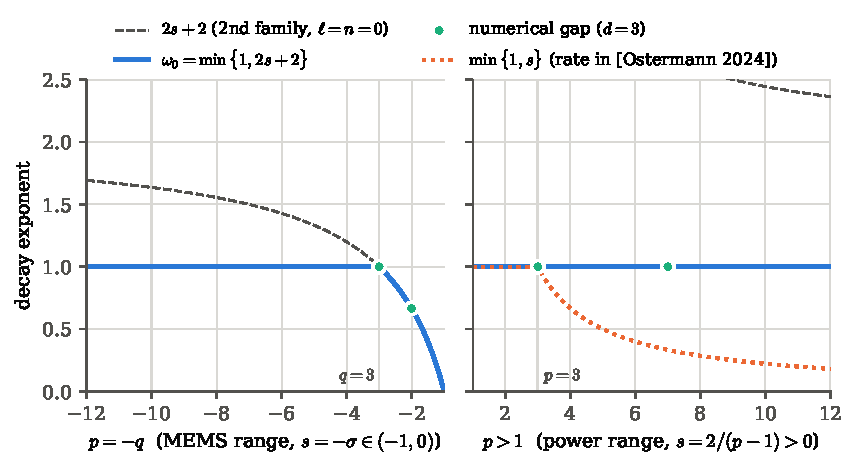
\includegraphics[width=0.92\textwidth]{figures/power_gap.pdf}
\caption{Spectral gap $\omega_0=\min\{1,2s+2\}$ over the MEMS range $p=-q<-1$
(left) and $p>1$ (right). Dashed: top of the second family, $2s+2$; dotted:
the exponent $\min\{1,s\}$ of \cite{Ostermann2024}, reflecting the free
eigenvalue $-s$; dots: numerically confirmed gaps ($d=3$).}
\label{power:fig-gap}
\end{figure}

\subsection{Summary and caveats}
\label{power:subsec-summary}

\textbf{(P)}: for all $p\notin[-1,1]$ (powers and MEMS), $V_0=(s+1)(s+2)$; the
spectrum in $\operatorname{Re}\lambda>-\omega_k$, $\omega_k=k-s_c$, is
$\{1-\ell-2n\}\cup\{-2s-2-\ell-2n\}$ with polynomial eigenfunctions; $\lambda=1$ and
the $d$-fold $\lambda=0$ are semisimple symmetry modes; the gap is
$\min\{1,2s+2\}$ ($=\frac23$ for $q=2$); Jordan blocks at $s=\pm\frac12$; no
self-similar ODE blowup for $-1\le p\le1$; the tilted family survives damping.
\textbf{(S)}: the free-flow splitting, the improved rate $1-\varepsilon$ for $p>1$,
\cref{power:lem-lower-order} and \cref{power:thm-lower-order}, conditional on the
autonomous linear estimate (for MEMS, \cref{mems:sec}). \textbf{(N)}: the
monodromy confirmation; Jordan blocks at all collisions; the co-dimension
claims of \cite{BizonMaisonWasserman2007}. Caveats: exponential decay needs
$k>s_c$ but the nonlinear argument uses $k>\frac d2$; the models are only valid up
to amplitudes where the cubic foundation law (or parallel-plate force) holds;
the literature in \cref{power:subsec-lit} was checked against abstracts, not
full texts.

\section{Geometric models: wave maps and relativistic membranes}
\label{geom:sec}

This section treats two \emph{geometric} wave equations: the wave map
($\sigma$-model) equation, which is semilinear and for which the Donninger
programme is essentially complete, and the timelike minimal-surface
(Nambu--Goto, scalar Born--Infeld) equation, which is quasilinear and for
which it is not. Throughout we separate
\textbf{(K)} known results (with references),
\textbf{(D)} what is derived or computed here (scripts
\texttt{code/geom\_*.py}), and
\textbf{(C)} conjectural statements.

\subsection{Wave maps: origin, scaling, and what is industrially relevant}
\label{geom:sec:wm-origin}

A wave map $\bm u:\mathbb{R}^{1+d}\to S^m\subset\mathbb{R}^{m+1}$ is a
critical point of $\frac12\int(|\partial_t\bm u|^2-|\nabla\bm u|^2)$ under
the constraint $|\bm u|=1$:
\begin{equation}\label{geom:eq:wm}
  \partial_t^2\bm u-\Delta\bm u=\bigl(|\nabla\bm u|^2-|\partial_t\bm u|^2\bigr)\bm u .
\end{equation}
\emph{Where it comes from.} (a) In the Ericksen--Leslie theory of nematic
liquid crystals with director inertia $\sigma_1$, one-constant Frank energy
$K$, frozen flow and no dissipation, the director $\bm n\in S^2$ obeys
\eqref{geom:eq:wm} with wave speed $c^2=K/\sigma_1$; unequal elastic
constants lead to the variational wave equations of Hunter and
Saxton~\cite{HunterSaxton1991}. (b) Inertial magnetisation dynamics
(nutation) has been observed in ferromagnetic films at sub-THz
frequencies~\cite{NeerajEtAl2021}; in antiferromagnets the leading-order
dynamics of the N\'eel vector is a nonlinear $\sigma$-model, i.e.\ a wave map
into $S^2$. % TODO verify: add a reference (Andreev--Marchenko / Haldane)
(c) In physics, the $O(4)$ $\sigma$-model ($m=3$, $d=3$) describes
cosmological textures; its collapse is the explicit self-similar solution of
Shatah~\cite{Shatah1988} and Turok--Spergel~\cite{TurokSpergel1990}.

\emph{Honest assessment.} In display-type liquid crystals the director
motion is overdamped and $\sigma_1$ is negligible, so \eqref{geom:eq:wm} is
a formal inertial limit. A damping term $\gamma\,\partial_t\bm u$ is, however,
a lower-order perturbation in similarity variables (relative size
$\gamma(T-t)$, cf.\ \cref{fw:subsec-lower}): \emph{if} a
singularity forms in the inertial regime, damping is asymptotically
irrelevant, and the inertial self-similar regime is entered only when
$T-t\ll\sigma_1/\gamma$. The scaling $\bm u\mapsto\bm u(\mu t,\mu x)$ ($s=0$)
leaves \eqref{geom:eq:wm} invariant and multiplies the energy by
$\mu^{2-d}$, so $d=2$ is energy critical and $d\ge3$ supercritical.
\begin{itemize}[leftmargin=*]
\item $d=2$ (films, planar magnets; target $S^2$): there is no
  self-similar blowup; energy cannot concentrate in the interior of the
  backward light cone \textbf{(K)}~\cite{ShatahTahvildarZadeh1992}, and
  equivariant blowup happens by bubbling off a harmonic map
  \cite{Struwe2003}, at non-self-similar (type~II) rates constructed in
  \cite{KriegerSchlagTataru2008} and shown to be stable within
  co-rotational symmetry in \cite{RaphaelRodnianski2012}. Donninger's
  method is \emph{not} the right tool there.
\item $d=3$, target $S^3$: self-similar blowup is generic and stable
  (\cref{geom:sec:wm-thm}). For the physically most relevant case
  \emph{$d=3$, target $S^2$} (bulk nematics, magnets) the co-rotational
  reduction below is unavailable; self-similar wave maps can still be
  sought as harmonic maps from hyperbolic space
  \cite{CazenaveShatahTahvildarZadeh1998}, but we are not aware of a
  stability theory for $S^2$ targets. What transfers is the method
  (similarity variables, mode stability without symmetry as in
  \cite{WeissenbacherKochDonninger2025,DonningerMoscatelli2026a}); what
  does not transfer is the explicit profile.
\end{itemize}

\subsection{Co-rotational wave maps and similarity variables}
\label{geom:sec:wm-setup}

For $m=d$ and the co-rotational ansatz
$\bm u(t,x)=(\sin u(t,r)\,\tfrac{x}{r},\cos u(t,r))$, $r=|x|$,
\eqref{geom:eq:wm} becomes
\begin{equation}\label{geom:eq:corot}
  u_{tt}-u_{rr}-\frac{d-1}{r}u_r+\frac{d-1}{2r^2}\sin(2u)=0 .
\end{equation}
\begin{proposition}[\textbf{K}; verified \textbf{D}]\label{geom:prop:profile}
For $d\ge3$, $u_T(t,r)=f_0\!\bigl(\frac{r}{T-t}\bigr)$ with
$f_0(\rho)=2\arctan\bigl(\rho/\sqrt{d-2}\bigr)$ solves \eqref{geom:eq:corot};
equivalently $f_0$ solves
$(\rho^2-1)f''+(2\rho-\tfrac{d-1}{\rho})f'+\tfrac{d-1}{2\rho^2}\sin 2f=0$
and is analytic on $[0,\infty)$, in particular across the light cone $\rho=1$.
\end{proposition}
This is due to Shatah and Turok--Spergel for $d=3$ and to
Bizo\'n--Biernat~\cite{BizonBiernat2015} for $d\ge4$; we checked it
symbolically for $3\le d\le 10$ (\texttt{geom\_wavemaps\_symbolic.py}).
For $d=3$, $f_0$ is the ground state of a family of smooth self-similar
solutions; numerically it attracts generic large data, and the first excited
one, which has exactly one unstable mode, sits at the threshold of blowup
\cite{BizonChmajTabor2000}.

\emph{Reduction to a semilinear radial equation.} Writing $u=r\psi$,
\eqref{geom:eq:corot} becomes (checked symbolically)
\begin{equation}\label{geom:eq:psi}
  \psi_{tt}-\Delta_{\mathbb{R}^{d+2}}\psi
  +\frac{d-1}{2r^3}\bigl(\sin(2r\psi)-2r\psi\bigr)=0,
\end{equation}
a radial wave equation on $\mathbb{R}^{d+2}$ with a smooth nonlinearity and
scaling exponent $s=1$. With $\psi_1=(T-t)\psi$, $\psi_2=(T-t)^2\psi_t$ and
$\xi\in\mathbb{B}^{d+2}$, the conventions of \cref{fw:sec} give an
\emph{autonomous} system, because
$(T-t)^3\frac{d-1}{2r^3}(\sin 2r\psi-2r\psi)
=\frac{d-1}{2|\xi|^3}(\sin 2|\xi|\psi_1-2|\xi|\psi_1)$.
The profile is $\psi_1=f_0(|\xi|)/|\xi|$. Linearising,
$\partial_\tau\Phi=(\mathbf L_0+\mathbf L')\Phi$ with
$\mathbf L'(\phi_1,\phi_2)=(0,-V\phi_1)$ and
\begin{equation}\label{geom:eq:V}
  V(\rho)=\frac{(d-1)(\cos 2f_0(\rho)-1)}{\rho^2}
         =-\frac{8(d-1)(d-2)}{(d-2+\rho^2)^2}\qquad(V=-\tfrac{16}{(1+\rho^2)^2}\text{ for }d=3).
\end{equation}
$\mathbf L'$ is compact on radial $\mathcal H_k:=H^k\times H^{k-1}(\mathbb{B}^{d+2})$.
For the free operator, the known Lumer--Phillips estimates (e.g.\
\cite{Donninger2011,ChatzikaleasDonningerGlogic2017,Glogic2025}) give a
growth bound $-\omega_k$ which, by scaling, should have
$\omega_k=k-\frac{d+2}{2}+1=k-\frac d2$ (the decay rate of \cref{fw:sec} with $s=1$
in dimension $d+2$).
\textbf{(D)} This value is sharp: for $\operatorname{Re}\lambda<-\omega_k$ both Frobenius branches at $\rho=1$,
$1$ and $(1-\rho^2)^{\frac{d-1}{2}-\lambda}$, lie in $H^k$ near $\rho=1$
(the second iff $\frac{d-1}{2}-\operatorname{Re}\lambda>k-\frac12$), so the
free mode regular at $\rho=0$ is an eigenfunction in $\mathcal H_k$ and every such
$\lambda$ is in the spectrum. Hence the spectrum of
$\mathbf L$ in $\{\operatorname{Re}\lambda>\frac d2-k\}$ consists of isolated
eigenvalues, and the regularity $k$ determines how much of it is visible.

\subsection{The spectral problem and how mode stability is proved}
\label{geom:sec:wm-spec}

Modes of the linearisation of \eqref{geom:eq:psi},
$\delta\psi=(T-t)^{-1-\lambda}g(\rho)$ (equivalently
$u-u_T\propto(T-t)^{-\lambda}\rho\,g(\rho)$, with the same $\lambda$), solve
\begin{equation}\label{geom:eq:mode}
  (1-\rho^2)g''+\Bigl(\frac{d+1}{\rho}-2(\lambda+2)\rho\Bigr)g'
  -(\lambda+1)(\lambda+2)g-V(\rho)g=0,\qquad 0<\rho<1 .
\end{equation}
The Frobenius exponents are $\{0,-d\}$ at $\rho=0$ and
$\{0,\sigma_2\}$, $\sigma_2=\frac{d-1}{2}-\lambda$, at $\rho=1$. We call
$\lambda$ an \emph{eigenvalue} if \eqref{geom:eq:mode} has a nonzero solution
in $C^\infty[0,1]$; for $\operatorname{Re}\lambda>\frac d2-k$ this coincides
with the eigenvalues of $\mathbf L$ on $\mathcal H_k$. Generically the
condition at $\rho=1$ excludes the $(1-\rho)^{\sigma_2}$ branch; when
$\sigma_2\in\mathbb N$ the exponent-$0$ branch may carry a logarithm, and if it
does not, the point $\rho=1$ imposes no condition at all.

\emph{Symmetry mode.} Time translation gives
$\partial_T u_T=-(T-t)^{-1}\rho f_0'(\rho)$, i.e.\ $\lambda=1$ with
$g_1=f_0'\propto(d-2+\rho^2)^{-1}$ (checked). Space translations and
Lorentz boosts leave the co-rotational class and appear only in the
non-symmetric problem. \emph{Mode stability} means: no eigenvalue with
$\operatorname{Re}\lambda\ge0$ except $\lambda=1$. The instability $\lambda=1$
is removed in the nonlinear argument by adjusting the blowup time $T$.

\begin{proposition}[Hyperbolic reformulation; \textbf{D}]\label{geom:prop:hyp}
Put $\rho=\tanh\eta$, $g=\cosh^{1+\lambda}(\eta)\,\chi(\eta)$,
$\kappa=\lambda-\frac{d-1}{2}$ and
$\psi_{\mathrm{1D}}=\sinh^{\frac{d+1}{2}}(\eta)\,\chi$. Then
\eqref{geom:eq:mode} is equivalent to
\begin{equation}\label{geom:eq:H}
  \Bigl(-\Delta_{\mathbb H^{d+2}}-\tfrac{(d+1)^2}{4}+W\Bigr)\chi=-\kappa^2\chi
  \iff
  H\psi_{\mathrm{1D}}:=-\psi_{\mathrm{1D}}''+Q\,\psi_{\mathrm{1D}}=-\kappa^2\psi_{\mathrm{1D}},
\end{equation}
with $W(\eta)=V(\tanh\eta)/\cosh^2\eta$ and
$Q=\frac{(d+1)(d-1)}{4\sinh^2\eta}+W$, a self-adjoint operator on
$L^2(0,\infty)$ \emph{independent of $\lambda$}. Smoothness of $g$ at
$\rho=1$ means $\psi_{\mathrm{1D}}=e^{-\kappa\eta}F(e^{-2\eta})$ with $F$
analytic at $0$, i.e.\ $\psi_{\mathrm{1D}}$ is the (analytically continued)
Jost solution.
\end{proposition}
\begin{proof}[Sketch]
Inside the backward light cone write $T-t=e^{-\sigma}\cosh\eta$,
$r=e^{-\sigma}\sinh\eta$; then the Minkowski metric equals
$e^{-2\sigma}(-d\sigma^2+g_{\mathbb H^{d+2}})$. Conformal covariance of the
conformal wave operator in dimension $d+3$, with scalar curvature
$-(d+2)(d+1)$ of $\mathbb H^{d+2}$, turns
$\psi_{tt}-\Delta\psi+V(\rho)(T-t)^{-2}\psi=0$ into
$\varphi_{\sigma\sigma}-\Delta_{\mathbb H}\varphi-\frac{(d+1)^2}{4}\varphi+W\varphi=0$
for $\varphi=e^{-\sigma(d+1)/2}\psi$; a mode is $\varphi=e^{\kappa\sigma}\chi(\eta)$.
We verified the resulting identity for \eqref{geom:eq:mode} symbolically and
at random complex $\lambda$ (\texttt{geom\_wavemaps\_symbolic.py}).
\end{proof}
\noindent\emph{Consequences.} (i) If $\operatorname{Re}\lambda>\frac{d-1}{2}$
then $\psi_{\mathrm{1D}}\in L^2$, so $-\kappa^2$ is an eigenvalue of $H$ and
$\lambda$ is \emph{real}; on $\operatorname{Re}\kappa=0$, $\kappa\neq0$ the Jost
function does not vanish. For $d=3$ the zero-energy solution regular at
$\eta=0$ is the gauge mode itself,
$\psi_{\mathrm{1D}}=\sinh^2\eta/\cosh2\eta>0$ (a threshold resonance), so
$H\ge0$ by Sturm's theorem: \emph{no eigenvalue with $\operatorname{Re}\lambda\ge1$
other than $\lambda=1$}. For $d\ge4$ the gauge mode is a positive solution of
$H\psi=-\kappa_1^2\psi$, $\kappa_1=\frac{3-d}{2}$, whence $H\ge-\kappa_1^2$
(Allegretto--Piepenbrink) and there are no eigenvalues $\lambda>d-2$; for
$\frac{d-1}{2}<\lambda\le d-2$ we counted the nodes of the zero-energy
solution numerically (none for $4\le d\le8$). (ii) In the strip
$0\le\operatorname{Re}\lambda<\frac{d-1}{2}$ the eigenvalues are
\emph{resonances} of $H$ (zeros of the continued Jost function with
$\operatorname{Re}\kappa<0$); no self-adjointness argument applies, and this is
where the difficulty of mode stability lies. For $d\ge4$ the gauge mode lies
inside this strip.

\begin{proposition}[Supersymmetric removal of the gauge mode; \textbf{D}]\label{geom:prop:susy}
Let $\psi_\star=\sinh^{\frac{d+1}{2}}\eta\,/\bigl((d-2)\cosh^2\eta+\sinh^2\eta\bigr)>0$
(the gauge mode) and $w=-\psi_\star'/\psi_\star$. Then
$H+\kappa_1^2=(-\partial_\eta+w)(\partial_\eta+w)$, and the partner
$\widetilde H=(\partial_\eta+w)(-\partial_\eta+w)-\kappa_1^2=H+2w'$ is, after
the substitutions of \cref{geom:prop:hyp} read backwards with $d+4$ in place of
$d+2$ and $\lambda+1$ in place of $\lambda$, the mode problem
\begin{equation}\label{geom:eq:susy}
  (1-\rho^2)h''+\Bigl(\frac{d+3}{\rho}-2(\lambda+3)\rho\Bigr)h'
  -(\lambda+2)(\lambda+3)h+\frac{4(d-1)}{d-2+\rho^2}\,h=0 .
\end{equation}
The intertwiner $\partial_\eta+w$ maps smooth modes of \eqref{geom:eq:mode}
to smooth modes of \eqref{geom:eq:susy} and annihilates the gauge mode; since
$(-\partial_\eta+w)(\partial_\eta+w)=\kappa_1^2-\kappa^2$ on modes, it is
injective for $\lambda\notin\{1,d-2\}$, and $\lambda=d-2$ is an eigenvalue of
neither problem. Hence
$\operatorname{spec}\eqref{geom:eq:susy}=\operatorname{spec}\eqref{geom:eq:mode}\setminus\{1\}$,
and mode stability is equivalent to the absence of eigenvalues of
\eqref{geom:eq:susy} with $\operatorname{Re}\lambda\ge0$.
\end{proposition}
The partner potential $-4(d-1)/(d-2+\rho^2)$ was found and checked
symbolically for $3\le d\le8$; the numerical spectra of
\eqref{geom:eq:mode} and \eqref{geom:eq:susy} agree to 20 digits except for
$\lambda=1$ (\cref{geom:tab:spec}). Removing the gauge mode by a Darboux
transformation in this spirit is the standard first step in the rigorous
proofs; we have not checked whether the cited works use exactly this
partner.
% TODO verify: compare with the transformation used in CostinDonningerXia2016 / CostinDonningerGlogic2017.

\emph{How the remaining strip is handled (K).} Donninger--Aichelburg
excluded real unstable eigenvalues other than $\lambda=1$
\cite{DonningerAichelburg2008}; Donninger--Sch\"orkhuber--Aichelburg
confined possible unstable eigenvalues to a compact set
\cite{DonningerSchoerkhuberAichelburg2012}; Costin--Donninger--Xia proved
mode stability for $d=3$ \cite{CostinDonningerXia2016} and
Costin--Donninger--Glogi\'c for all $d\ge4$ \cite{CostinDonningerGlogic2017}.
In outline (as we understand it), the \emph{quasi-solution method} of the
latter works with the power series of the solution regular at the origin
(after removal of the gauge mode): $\lambda$ is an eigenvalue iff that series
converges beyond $\rho=1$. The coefficients satisfy a finite-term
recurrence; one writes down an explicit approximate solution (the
quasi-solution) for the ratio of consecutive coefficients and controls the
error rigorously, showing that the ratio tends to $1$ for all
$\operatorname{Re}\lambda\ge0$. The radius of convergence is then $1$, and if
$\rho=1$ is the only singular point of the equation on the unit circle, the
solution must be singular there. \emph{Observation (D):} this last step is
where $d=3$ differs: the potential \eqref{geom:eq:V} has poles at
$\rho=\pm i$, on the unit circle, whereas for $d\ge4$ the poles
$\pm i\sqrt{d-2}$ lie outside it (the same holds for the partner
potential in \eqref{geom:eq:susy}).

\subsection{Numerically computed spectrum}
\label{geom:sec:wm-num}

We used three independent methods (\texttt{geom\_modes.py},
\texttt{geom\_wavemaps\_spectrum.py}): (1) Chebyshev collocation in
$y=\rho^2$ with $N=40,\dots,120$ nodes, without boundary conditions (both ends
are singular points), linearising the quadratic pencil; (2) Frobenius series
about $y=0$ and $y=1$ (400 terms, 30--35 digits), whose Wronskian at
$y=\frac12$, multiplied by $1/\Gamma(1-\sigma_2)$, is an \emph{entire}
function of $\lambda$ whose zeros are exactly the eigenvalues (the factor
removes the poles at $\sigma_2\in\mathbb N$, and log-free resonances are zeros
automatically), refined by Newton's method; (3) the argument principle for
this Wronskian on the rectangle
$[-1.9,4]\times[-15,15]$ ($1200$ points, maximal phase step $<0.6$\,rad).
\begin{table}[ht]
\centering\footnotesize
\begin{tabular}{@{}llll@{}}
\toprule
 & $d=3$ & $d=4$ & $d=5$\\
\midrule
gauge & $1$ & $1$ & $1$\\
$\lambda_1$ & $-0.54246\,63534\,31726\,5370$ & $-0.56361\,26748\,07079\,4374$ & $-0.57231\,57218\,74117\,6664$\\
$\lambda_2$ & $-2$ (exact) & $-2.10913\,10073\,42525\,1316$ & $-2.16301\,19522\,28281\,9288$\\
winding \eqref{geom:eq:mode}/\eqref{geom:eq:susy} & $2\,/\,1$ & $2\,/\,1$ & $2\,/\,1$\\
\bottomrule
\end{tabular}
\caption{Eigenvalues of \eqref{geom:eq:mode} with $\operatorname{Re}\lambda\ge-2.2$
(Wronskian method; digits stable under changes of truncation and precision).
Collocation reproduces $\lambda_1$ to $10^{-8}$ for $N=40$--$80$ (round-off
grows for larger $N$). The last row is the winding number of the Wronskian on
$[-1.9,4]\times[-15,15]$ for the original and the SUSY-partner problem.}
\label{geom:tab:spec}
\end{table}

\begin{figure}[ht]
\centering
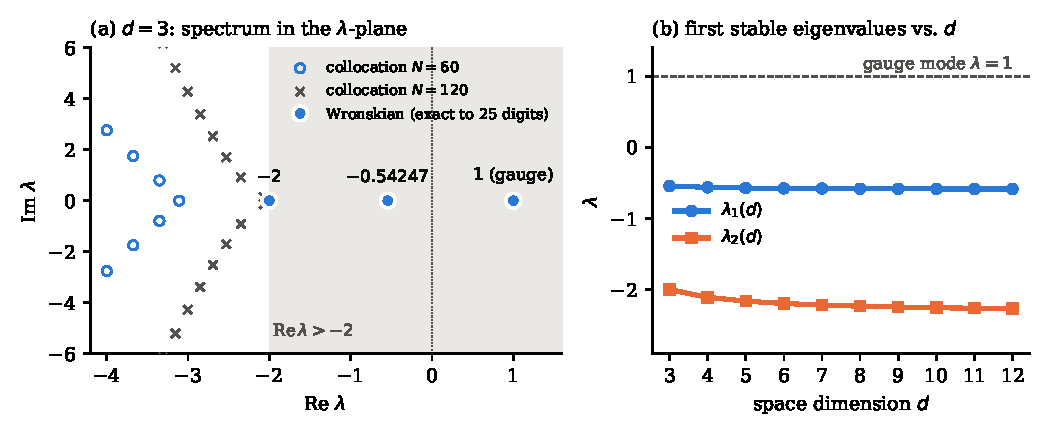
\includegraphics[width=\textwidth]{figures/geom_spectrum.pdf}
\caption{(a) $d=3$: collocation eigenvalues for $N=60$ (circles) and
$N=120$ (crosses) and the eigenvalues confirmed by the Wronskian (filled).
Collocation values with $\operatorname{Re}\lambda\lesssim-2$ move with $N$;
they come from the branch $(1-\rho^2)^{\sigma_2}$ with
$\operatorname{Re}\sigma_2\gtrsim3$, which polynomials cannot distinguish
from smooth functions at finite $N$, and they are rejected by the
Wronskian. They mirror the fact that on $\mathcal H_k$ the half-plane
$\operatorname{Re}\lambda<\frac d2-k$ is spectrum. (b) The first two stable
eigenvalues for $3\le d\le12$.}
\label{geom:fig:spec}
\end{figure}

\textbf{Findings (D).} (1) For $d=3,4,5$ the only eigenvalues in
$[-1.9,4]\times[-15,15]$ are the gauge mode and one real stable eigenvalue
$\lambda_1(d)$, and the only one in $[-2.25,-1.95]\times[-6,6]$ is
$\lambda_2(d)$ (argument principle); together with consequence~(i) of
\cref{geom:prop:hyp} for large real parts and the known exclusion of large imaginary parts
\cite{DonningerSchoerkhuberAichelburg2012} this is a numerical confirmation
of mode stability with spectral gap $|\lambda_1|$. (2) $\lambda_1(d)$
decreases slowly from $-0.5425$ ($d=3$) to $-0.5865$ ($d=12$). (3) For $d=3$,
$\lambda=-2$ is an eigenvalue with the explicit, analytic eigenfunction (in
the $u$-picture, $u-u_T\approx\varepsilon(T-t)^2\phi(\rho)$)
\[
  \phi(\rho)=\frac{3(1+\rho^2)^3\arctan\rho-3\rho-4\rho^3-9\rho^5}{\rho^2(1+\rho^2)},
\]
checked symbolically; here $\sigma_2=3$ and the Frobenius recursion at
$\rho=1$ turns out to be log-free, so $\rho=1$ imposes no condition. We know
no symmetry interpretation. (4) Consequently, in $\mathcal H_k$ with
$k>\frac d2+|\lambda_1|$, perturbations (after fixing $T$) should decay like
$e^{-\omega\tau}=(T-t)^{\omega}$ for every $\omega<|\lambda_1|$, i.e.\
$(T-t)^{0.54}$ for $d=3$. For $k=2$ and $d=3$ the free decay rate
$\omega_2=\frac12$ is the binding constraint, since $|\lambda_1|>\frac12$.

\subsection{Known stability theorems}
\label{geom:sec:wm-thm}

\begin{theorem}[\textbf{K}: Donninger \cite{Donninger2011};
Donninger--Sch\"orkhuber--Aichelburg \cite{DonningerSchoerkhuberAichelburg2012};
Costin--Donninger--Xia \cite{CostinDonningerXia2016}]\label{geom:thm:d3}
Let $d=3$. There are $\varepsilon,\delta>0$ such that for co-rotational data
$(u(0,\cdot),u_t(0,\cdot))$ that are $\varepsilon$-close to
$(f_0(r),rf_0'(r))$ (the profile with $T=1$) in a radial Sobolev norm of
sufficiently high regularity on the ball $\{r<1+\delta\}$, there is
$T\in(1-\delta,1+\delta)$ such that the solution blows up at $(T,0)$ and,
in similarity variables on the backward light cone of $(T,0)$, converges to
the profile $f_0$ exponentially in $\tau=-\log(T-t)$.
\end{theorem}
\cite{Donninger2011} proves this assuming mode stability,
\cite{DonningerSchoerkhuberAichelburg2012} develops the linear theory, and
\cite{CostinDonningerXia2016} proves mode stability, which makes the theorem
unconditional. Further results (all \textbf{K}):
\begin{itemize}[leftmargin=*,itemsep=1pt]
\item odd $d$: nonlinear stability of $f_0$
  \cite{ChatzikaleasDonningerGlogic2017}, using mode stability from
  \cite{CostinDonningerGlogic2017};
\item $d=3$, stability in the whole space (hyperboloidal similarity
  coordinates, evolution followed past the blowup time almost up to the
  Cauchy horizon) \cite{BiernatDonningerSchoerkhuber2021}; all $d\ge3$,
  global-in-space stability \cite{Glogic2025};
\item stability under perturbations small only in the critical Sobolev
  space: $d=4$ \cite{DonningerWallauch2023}; $d=3$, fractional critical space,
  via Strichartz estimates in similarity coordinates
  \cite{DonningerWallauch2025};
\item without any symmetry: mode stability for $d=3$
  \cite{WeissenbacherKochDonninger2025} and $d\ge4$
  \cite{DonningerMoscatelli2026a} (quasi-solution method with two extra
  parameters), and asymptotic stability \cite{DonningerMoscatelli2026b}
  (preprints). % TODO verify: dimension range and data space of DonningerMoscatelli2026b
\end{itemize}

\subsection{Relativistic membranes and the scalar Born--Infeld equation}
\label{geom:sec:membranes}

A timelike hypersurface $M^{d+1}\subset\mathbb{R}^{1,d+1}$ with vanishing
mean curvature (Nambu--Goto membrane; $d=1$ strings, $d=2$ membranes) is,
as a graph $z=u(t,x)$, a critical point of $-\int L$,
$L=\sqrt{1-u_t^2+|\nabla u|^2}$:
\begin{equation}\label{geom:eq:BI}
  \partial_t\Bigl(\frac{u_t}{L}\Bigr)-\nabla\!\cdot\!\Bigl(\frac{\nabla u}{L}\Bigr)=0
  \iff
  (1+|\nabla u|^2)u_{tt}-2u_t\nabla u\!\cdot\!\nabla u_t-L^2\Delta u+u_iu_ju_{ij}=0 ,
\end{equation}
the scalar Born--Infeld equation (the equivalence, after multiplication by
$L^3$, was checked in the radial case). It is quasilinear, hyperbolic
while $L^2>0$, and degenerates when $M$ becomes null. The scaling
$u\mapsto\mu^{-1}u(\mu t,\mu x)$ gives $s=-1$, so self-similar solutions are
$u=(T-t)U(x/(T-t))$: bounded slopes, curvature $\sim(T-t)^{-1}$.

\emph{Literature (K).} Eggers--Hoppe derived self-similar string solutions
in a graph representation near singularities (of swallowtail type) and their
extension to point singularities of membranes \cite{EggersHoppe2009};
Eggers--Hoppe--Hynek--Suramlishvili relate membrane singularities to
caustics of the eikonal equation and observe them numerically, e.g.\ at the
poles of collapsing ellipsoids \cite{EggersEtAl2015}. Nguyen--Tian show that
timelike maximal cylinders in $\mathbb{R}^{1+2}$ become singular in finite
time and, near a generic singularity, move rigidly or self-similarly
\cite{NguyenTian2013}. Wong proved that axially symmetric timelike minimal submanifolds (in the
class considered there) cannot exist globally in time, and analysed the
limiting geometry \cite{Wong2018}; Cai--Liu
construct radial singularities through loss of hyperbolicity (the surface
turns null) \cite{CaiLiu2025}. On the stability side,
Donninger--Krieger--Szeftel--Wong proved codimension-one stability of the
(static, non-singular) catenoid \cite{DonningerEtAl2016}, and
Bahouri--Marachli--Perelman constructed type~II blowup near the Simons cone,
adapting the Krieger--Schlag--Tataru method to this quasilinear setting
\cite{BahouriMarachliPerelman2021}. Yan proposed explicit ``lightlike''
self-similar solutions $u=\pm(T-t)\sqrt{1-\rho^2}$ and stability statements
in a proper subregion of the backward light cone
\cite{Yan2017,Yan2019b} (and for the $1{+}1$ Born--Infeld equation
\cite{Yan2019a}); see \cref{geom:prop:cone}(c) for what these solutions
are. We found no Donninger-type stability result for a \emph{timelike}
self-similar membrane singularity, nor for Born--Infeld blowup beyond
these preprints (literature search of October 2026, which had to stop
before every lead was exhausted).

\begin{proposition}[Self-similar membranes are minimal cones; \textbf{D}]
\label{geom:prop:cone}
Let $p=(T,0,0)$. Inside the backward light cone of $p$ the map
$(t,x,z)\mapsto(x,z)/(T-t)\in\mathbb{B}^{d+1}$ is the Beltrami--Klein model of
$\mathbb H^{d+1}$, and these are exactly the similarity coordinates.
\begin{enumerate}[label=(\alph*),leftmargin=*,itemsep=1pt]
\item The graph of $u=(T-t)U(\xi)$ is, inside the light cone of $p$, the
  cone $C(\Sigma)$ with vertex $p$ over
  $\Sigma=\{(\xi,U(\xi))\}\cap\mathbb{B}^{d+1}$; it solves
  \eqref{geom:eq:BI} iff $\Sigma$ is a minimal hypersurface of $\mathbb H^{d+1}$.
\item Normal perturbations $\varphi=\ell^{a}\chi(\omega)$, $\ell$ = proper
  time to $p$, solve the Jacobi equation $\Box_{C}\varphi+|\mathrm{II}_C|^2\varphi=0$
  iff $J_\Sigma\chi=(a-1)(a+d)\chi$, where
  $J_\Sigma=\Delta_\Sigma+|A_\Sigma|^2-d$ is the Jacobi operator of
  $\Sigma\subset\mathbb H^{d+1}$. In similarity variables $\lambda=1-a$:
  \[-J_\Sigma\chi=\lambda(d+1-\lambda)\chi .\]
  Translations give $\lambda=1$ ($\chi=\langle\nu,e\rangle$,
  $J_\Sigma\chi=-d\chi$); Lorentz transformations fixing $p$ give $\lambda=0$
  (Killing--Jacobi fields).
\item Consequences: for $d=1$ every self-similar string is a plane
  (geodesics of $\mathbb H^2$); every \emph{radial} self-similar graph regular at
  $\xi=0$ is $U\equiv c$, a plane moving with constant velocity (a minimal
  hypersurface of revolution meeting the axis is totally geodesic; the Taylor
  recursion of the radial ODE confirms $U''(0)=U^{(4)}(0)=\dots=0$ for
  $d=1,2,3$). The solutions $\pm(T-t)\sqrt{1-|x|^2/(T-t)^2}$ correspond to
  $\Sigma=\partial_\infty\mathbb H^{d+1}$: they satisfy the non-divergence
  form of \eqref{geom:eq:BI} but have $L\equiv0$, i.e.\ they are \emph{null}
  cones, where the equation is not hyperbolic (checked).
\end{enumerate}
\end{proposition}
\begin{proof}[Sketch]
The induced metric of $C(\Sigma)$ is $-d\ell^2+\ell^2g_\Sigma$, the radial
direction is geodesic and $\mathrm{II}_C=\ell\,\mathrm{II}_\Sigma$ on
$T\Sigma$, so $H_C=\ell^{-1}H_\Sigma$ and $|\mathrm{II}_C|^2=\ell^{-2}|A_\Sigma|^2$.
With $\Box_C=-\ell^{-d}\partial_\ell(\ell^d\partial_\ell)+\ell^{-2}\Delta_\Sigma$
one gets $(\Delta_\Sigma+|A_\Sigma|^2)\chi=a(a+d-1)\chi$, and
$\mathrm{Ric}_{\mathbb H^{d+1}}(\nu,\nu)=-d$. For $\Sigma=\mathbb H^d$ (the flat
membrane) this reproduces the free eigenvalues $\lambda\in\{1,0,-1,\dots\}$
of \cref{fw:sec} with $s=-1$, $V_0=0$. This is the membrane analogue of the
correspondence between self-similar wave maps and harmonic maps from
$\mathbb H^d$ \cite{CazenaveShatahTahvildarZadeh1998} and of
\cref{geom:prop:hyp}.
\end{proof}

\emph{Shrinking spheres (D).} A round $k$-sphere $R(t)\omega$ in
$\mathbb{R}^{k+1}$ ($k=1$ string, $k=2$ membrane) has Lagrangian
$-R^k\sqrt{1-R_t^2+|\nabla_{S^k}R|^2/R^2}$ (determinant of the induced metric
checked for $k=2$). Homogeneous solutions conserve
$E=R^k/\sqrt{1-\dot R^2}$; for $k=1$, $R=E\cos(t/E)$. Every such sphere
collapses at a finite time $T$ with $\dot R\to-1$ and Lorentz factor
$E/R^k\to\infty$:
\[
  R(t)=(T-t)-\frac{(T-t)^{2k+1}}{2(2k+1)E^2}+O\bigl((T-t)^{4k+1}\bigr).
\]
In similarity variables $R/(T-t)\to1$: the collapse is \emph{lightlike}; the
limiting profile is the null cone of \cref{geom:prop:cone}(c), sitting on the
boundary $|\xi|=1$ of the similarity domain. Linearising about it,
$R=R_0+\varepsilon\sum\delta_{\ell}(t)Y_{\ell}$ gives (derived and checked)
\begin{equation}\label{geom:eq:sphere-lin}
  \ddot\delta_\ell-2k\frac{\dot R_0}{R_0}\dot\delta_\ell
  +\frac{\ell(\ell+k-1)-k}{E^2}R_0^{2k-2}\delta_\ell=0 ,
\end{equation}
whose exponents at $t=T$ are $0$ and $2k+1$. Hence generically
$\delta_\ell(T)\ne0$ and $\delta_\ell/R_0\sim(T-t)^{-1}$: in similarity
variables \emph{every} harmonic $(\ell,m)$ has a mode with $\lambda=1$ (and
one with $\lambda=-2k$). Only $\ell=0$ (time shift) and $\ell=1$
(translations) are symmetries; for instance, for $k=2$, $E=1$, data
$(\delta_\ell,\dot\delta_\ell)=(0,1)$ at rest we find
$\delta_\ell(T)=0.5,\,0.437,\,0.328,\,0.2,\,0.083$ for $\ell=0,\dots,4$
(\texttt{geom\_membrane.py}). Geometrically, each ray of the
ultra-relativistic membrane reaches the centre at its own time: the round
focus is an infinitely degenerate caustic which generic perturbations
unfold, in line with the caustic picture of \cite{EggersEtAl2015}. Spherical
collapse is therefore unstable in infinitely many directions, and a
Donninger-type argument (finite-dimensional instabilities removed by
modulation) cannot apply to it.

\subsection{Assessment and open problems}
\label{geom:sec:assess}

\begin{enumerate}[leftmargin=*,itemsep=2pt]
\item \textbf{Wave maps (K + D).} The Donninger programme is complete for
  co-rotational wave maps into $S^d$, $d\ge3$, and is now being extended
  beyond symmetry. Our computations reproduce the spectral picture
  (gauge mode $\lambda=1$, gap $|\lambda_1|\approx0.54$--$0.59$), give a
  self-contained proof of the absence of eigenvalues with
  $\operatorname{Re}\lambda\ge\frac{d-1}{2}$ other than the gauge mode for $d=3$
  (consequence~(i) of \cref{geom:prop:hyp}), and give an explicit SUSY partner
  \eqref{geom:eq:susy}. The open cases relevant for applications are $d=2$
  with target $S^2$ (bubbling, not self-similar, so a different theory) and
  $d=3$ with target $S^2$, where neither the profile nor its stability is
  settled as far as we know.
\item \textbf{Membranes: obstacles (D).} (a) \emph{Quasilinearity:} the
  perturbation $\mathbf L'$ contains second derivatives, so it is not compact
  relative to $\mathbf L_0$, and the domain of dependence moves with the
  solution. One needs energy estimates adapted to the background's
  characteristic cone; this has not been done in similarity variables.
  (b) \emph{Characteristic degeneracy:} the singularities found so far in
  analysis and numerics (strings, spheres, axisymmetric membranes) are
  lightlike, and then the
  similarity variables put the profile on the boundary $|\xi|=1$. (c)
  \emph{Gauge:} the graph gauge fails where the surface turns vertical
  (swallowtails); normal graphs over the cone are the natural choice in
  \cref{geom:prop:cone}.
\item \textbf{Where a Donninger-type theory is plausible (C).} Timelike
  self-similar membranes are cones over minimal hypersurfaces
  $\Sigma\subset\mathbb H^{d+1}$. Such $\Sigma$ with prescribed ideal
  boundary exist in abundance by classical results on the asymptotic
  Plateau problem in hyperbolic space.
  % TODO verify refs: Anderson (asymptotic Plateau problem); Hardt--Lin (regularity at infinity)
  The questions are whether some non-flat $\Sigma$ extends
  \emph{smoothly} across the ideal boundary in the Klein coordinates, i.e.\
  across the light cone of $p$, which is the analogue of the selection of
  $f_0$ by smoothness at $\rho=1$, and whether the resonances of $J_\Sigma$
  in \cref{geom:prop:cone}(b) satisfy mode stability. Boundary expansions of
  minimal submanifolds in hyperbolic space suggest that a generic $\Sigma$
  has a non-smooth term of order $(1-|\xi|^2)^{(d+1)/2}$ (with a logarithm
  for odd $d$), so smooth cones, if they exist, are isolated. We have not
  verified this.
\item \textbf{Industrial relevance (honest).} Nambu--Goto and Born--Infeld
  are physics models (strings and branes, nonlinear electrodynamics). The
  engineering large-deflection membrane
  $\rho_h u_{tt}=\mathcal T\,\nabla\!\cdot(\nabla u/\sqrt{1+|\nabla u|^2})$
  shares the scaling $s=-1$ but is not Lorentz invariant and is hyperbolic
  for every slope, with squared wave speeds
  $\mathcal T/(\rho_h W)$ and $\mathcal T/(\rho_h W^3)$, $W=\sqrt{1+|\nabla u|^2}$,
  so there is no null degeneration (the speeds degenerate only as
  $|\nabla u|\to\infty$). We know of no self-similar blowup result
  for it; in MEMS the dominant membrane nonlinearity is usually stretching,
  not slope.
\end{enumerate}

\section{Nonlinear acoustics and derivative nonlinearities}
\label{acou:sec}

High-intensity ultrasound (HIFU tissue ablation, shock-wave lithotripsy,
ultrasonic cleaning and welding) and sonic-boom propagation are described, to
second order in the acoustic Mach number, by the Westervelt and Kuznetsov
equations \cite{HamiltonBlackstock1998,Kaltenbacher2015}. Their
nonlinearities are quadratic in \emph{derivatives} of the unknown and they are
quasilinear. We ask which of these models, and two semilinear caricatures,
show ODE-type self-similar blowup, and how far the method of \cref{fw:sec}
carries. As in \cref{geom:sec} we mark statements as
\textbf{(K)} known (with reference), \textbf{(D)} derived or proved here
(proof or proof sketch given, formulas checked in
\texttt{code/acou\_symbolic.py}), \textbf{(C)} conjectural, formal or
numerical only.

\subsection{Models}
\label{acou:sub-models}
\textbf{(K)} With acoustic pressure $p$, velocity potential $\psi$, ambient
density $\rho_0$, sound speed $c$, coefficient of nonlinearity
$\beta=1+B/(2A)$ and diffusivity of sound $b$, the Westervelt equation in
pressure form reads
\begin{equation}\label{acou:west}
  (1-2kp)\,p_{tt}-c^2\Delta p-b\Delta p_t=2k\,(p_t)^2,\qquad
  k=\frac{\beta}{\rho_0c^2},
\end{equation}
i.e.\ $p_{tt}-c^2\Delta p-b\Delta p_t=k(p^2)_{tt}$. It is obtained by
applying $\partial_t$ to the potential form
$\psi_{tt}-c^2\Delta\psi-b\Delta\psi_t=\beta c^{-2}\partial_t(\psi_t^2)$ and
setting $p=\rho_0\psi_t$. The Kuznetsov equation is
\begin{equation}\label{acou:kuz}
  \psi_{tt}-c^2\Delta\psi-b\Delta\psi_t
  =\partial_t\big(K\psi_t^2+|\nabla\psi|^2\big),\qquad K=\frac{B}{2A}\,c^{-2}
\end{equation}
\cite{Kuznetsov1971,Westervelt1963,Kaltenbacher2015}.
% TODO verify: bibliographic data of Kuznetsov1971, Westervelt1963, HamiltonBlackstock1998 (bib/acou.bib, from memory)
\textbf{(D)} The two
right-hand sides differ exactly by
$\partial_t\big(|\nabla\psi|^2-c^{-2}\psi_t^2\big)$, the time derivative of
the (negative) \emph{null form} $Q_0(\psi,\psi)$: the classical argument that
``local nonlinear effects'' are negligible for progressive waves is the
statement that $Q_0$ vanishes on plane waves.

\emph{Nondimensionalisation.} With $u=2kp$, $t\mapsto t_0t$, $x\mapsto ct_0x$,
\eqref{acou:west} becomes
\begin{equation}\label{acou:west-nd}
  (1-u)\,u_{tt}-\Delta u-\varepsilon\Delta u_t=(u_t)^2,\qquad
  \varepsilon=\frac{b}{c^2t_0}.
\end{equation}
For water ($\rho_0c^2\approx2.2\,$GPa, $\beta\approx3.5$,
$b\approx4\times10^{-6}\,\mathrm{m^2/s}$; standard handbook values, cf.\
\cite{HamiltonBlackstock1998}) the degeneracy $u=1$ corresponds to
$p^\ast=\rho_0c^2/(2\beta)\approx 3\times10^{2}\,$MPa, and the viscous time
scale is $b/c^2\approx2\times10^{-12}\,$s.

\emph{Two semilinear caricatures.} Freezing the coefficient $1-u$ to $1$ and
setting $\varepsilon=0$ in \eqref{acou:west-nd} gives the \emph{Riccati wave
equation}; replacing $(u_t)^2$ by the null form gives Nirenberg's example:
\begin{equation}\label{acou:models}
  \text{(RW)}\quad u_{tt}-\Delta u=(u_t)^2,\qquad\qquad
  \text{(NF)}\quad u_{tt}-\Delta u=(u_t)^2-|\nabla u|^2 .
\end{equation}
(RW) keeps the ``cumulative'' part $2kp_t^2$ of $k(p^2)_{tt}=2kpp_{tt}+2kp_t^2$
and drops the quasilinear part; (NF) is the semilinear analogue of the local
nonlinear effects.

\subsection{Shocks versus ODE-type blowup}
\label{acou:sub-which}
\textbf{(K)} For propagating waves the generic singularity is a shock: in
1D, simple waves of \eqref{acou:west} obey Burgers' equation and steepen at
the shock-formation distance while $p$ stays bounded
\cite{HamiltonBlackstock1998}; in several dimensions shock formation for
quasilinear wave equations is a different, geometric theory
\cite{Christodoulou2007}. % TODO verify bib data of Christodoulou2007 (from memory)
Shocks are not ODE-type blowup and lie outside the
semigroup method. ODE-type blowup instead requires a spatially
\emph{coherent} drive (in phase over a region larger than $c(T-t)$), such as
a uniform compression. \textbf{(D)} The spatially homogeneous dynamics are:
\begin{itemize}[nosep]
\item (RW), (NF): $u_T(t)=-\log(T-t)+c_0$ (exact), so that $u$ and $u_t$ blow up.
\item Westervelt, $b=0$: with $q:=1-2kp$, \eqref{acou:west} is equivalent to
  \begin{equation}\label{acou:qeq}
    (q^2)_{tt}=2c^2\Delta q .
  \end{equation}
  Homogeneous solutions have $q^2=A(T-t)$ (plus a constant), so
  $p\to1/(2k)$ stays bounded while $p_t=\sqrt A/(4k\sqrt{T-t})$. This is a
  \emph{degeneration}, not a blowup of $p$: the coefficient of $p_{tt}$
  vanishes and the local sound speed $c/\sqrt q$ becomes infinite.
\item Kuznetsov, $b=0$: $\psi=\psi(t)$ forces $(1-2K\psi_t)\psi_{tt}=0$, so
  there is \emph{no} homogeneous blowup, Riccati-type or otherwise (the
  right-hand side of \eqref{acou:kuz} is a total time derivative). The
  uniform compression $\psi=f(t)+B_0|x|^2/(2dc^2)$, whose velocity field is
  linear in $x$, solves \eqref{acou:kuz} if and only if
  $(f'-Kf'^2)'=B_0$, and it reaches the same degeneracy $\psi_t\to1/(2K)$
  with $\psi_{tt}\sim(T-t)^{-1/2}$.
\end{itemize}
The remaining subsections treat (RW) (\cref{acou:sub-rw,acou:sub-spec,acou:sub-nonlin}),
(NF) (\cref{acou:sub-nf}), the degenerate Westervelt blowup
(\cref{acou:sub-west}) and the role of $b$ (\cref{acou:sub-visc}).

\subsection{The Riccati wave equation: symmetries, tilted blowup, similarity variables}
\label{acou:sub-rw}
\textbf{(D)} (RW) is invariant under translations, rotations, the scaling
$u\mapsto u(\mu t,\mu x)$ and the \emph{shift} $u\mapsto u+c_0$. It is
\emph{not} Lorentz invariant, because $(u_t)^2$ is not.

\begin{lemma}[tilted ODE blowup]\label{acou:lem-tilt}
For $a\in\mathbb R^d$, $|a|<1$, and $c_0\in\mathbb R$,
\[
  u_{T,a}(t,x)=-(1-|a|^2)\log\big(T-t+a\cdot x\big)+c_0
\]
solves (RW) on $\{T-t+a\cdot x>0\}$. It blows up on the spacelike hyperplane
$t=T+a\cdot x$, with $\partial_tu_{T,a}=(1-|a|^2)/(T-t+a\cdot x)$. Among the
functions $-C\log(T-t+a\cdot x)$ with $C\ne0$, the coefficient $C=1-|a|^2$ is the only one that gives a solution.
\end{lemma}
\begin{proof}
With $f=T-t+a\cdot x$ one has $\Box(-C\log f)=C(1-|a|^2)f^{-2}$ and
$(\partial_t(-C\log f))^2=C^2f^{-2}$.
\end{proof}
So the pointwise blowup rate depends on the slope of the blowup surface: if
a solution blows up on $t=T(x)$, the local ansatz $u\approx-C(x)\log(T(x)-t)$
gives $C(x)=1-|\nabla T(x)|^2$. For (NF) the analogous family is
$-\log(T-t+a\cdot x)$ with coefficient $1$, the Lorentz boosts of $u_T$.

\emph{Similarity variables.} With $\tau,\xi$ as in \cref{fw:sec} let
\[
  \psi_1=u+\log(T-t),\qquad \psi_2=(T-t)\,\partial_tu .
\]
Then (RW) is equivalent to
\begin{equation}\label{acou:sys}
  \partial_\tau\psi_1=-\Lambda\psi_1+\psi_2-1,\qquad
  \partial_\tau\psi_2=\Delta\psi_1-\Lambda\psi_2-\psi_2+\psi_2^2 ,
\end{equation}
with equilibria $(c_0,1)$ (the ODE blowup). In these variables the tilted
solutions read, with $T=1$,
\begin{equation}\label{acou:tilt-sim}
  \psi_1=-|a|^2\tau-(1-|a|^2)\log(1+a\cdot\xi)+c_0,\qquad
  \psi_2=\frac{1-|a|^2}{1+a\cdot\xi}.
\end{equation}
They are stationary in $(\nabla\psi_1,\psi_2)$, while $\psi_1$ drifts
linearly in $\tau$. Since \eqref{acou:sys} contains $\psi_1$ only through
$\nabla\psi_1$, the natural phase space is the quotient by constants
\[
  \mathcal H^k:=\big(H^k\times H^{k-1}(B^d)\big)\big/\mathbb R(1,0),\qquad
  \|[\Phi]\|:=\|\nabla\phi_1\|_{H^{k-1}}+\|\phi_2\|_{H^{k-1}} .
\]
In $\mathcal H^k$ the tilted solutions form a $d$-parameter family of
equilibria $\Phi_a$.

\emph{Linearisation.} Writing $\Psi=(c_0,1)+\Phi$,
\begin{equation}\label{acou:lin}
  \partial_\tau\Phi=\mathbf L\Phi+\mathbf N(\Phi),\qquad
  \mathbf L\Phi=\begin{pmatrix}-\Lambda\phi_1+\phi_2\\ \Delta\phi_1-\Lambda\phi_2+\phi_2\end{pmatrix},\qquad
  \mathbf N(\Phi)=\begin{pmatrix}0\\ \phi_2^2\end{pmatrix}.
\end{equation}
Thus $\mathbf L=\mathbf L_0^{(0)}+\mathbf L'$ with $\mathbf L'\Phi=(0,2\phi_2)$.
Unlike $(0,V_0\phi_1)$ for $F=F(u)$, the operator $\mathbf L'$ is bounded but
\emph{not compact} on $H^k\times H^{k-1}$, because it gains no derivative.
This is the generic obstruction for derivative nonlinearities, and Step~2 of
\cref{fw:subsec-steps} fails as stated. For (RW) the problem disappears
because of an exact identity.

\begin{lemma}[exact conjugation]\label{acou:lem-conj}
Let $\mathbf S(f_1,f_2)=(f_1,f_1+f_2)$, which is bounded with bounded inverse
on $H^k\times H^{k-1}(B^d)$. Then
$\mathbf L=\mathbf S\,\mathbf L_0^{(-1)}\mathbf S^{-1}$. In physical variables,
$v$ solves the linearised equation $v_{tt}-\Delta v=2(T-t)^{-1}v_t$ if and
only if $w=(T-t)v$ solves $\Box w=0$.
\end{lemma}
\begin{proof}
$\mathbf L\mathbf S(f_1,f_2)=(-\Lambda f_1+f_1+f_2,\ \Delta f_1-\Lambda f_1+f_1-\Lambda f_2)
=\mathbf S\mathbf L_0^{(-1)}(f_1,f_2)$. In physical variables,
$(T-t)\big(v_{tt}-\Delta v-\tfrac{2}{T-t}v_t\big)=\Box\big((T-t)v\big)$.
\end{proof}
At the linear level, (RW) is therefore a free wave equation with
\emph{effective scaling exponent $s=-1$}. This is precisely the borderline
case excluded in \cref{fw:thm-spec}: at $s=-1$ the second family
$-2s-2-\ell-2n$ reaches $0$ at $\ell=n=0$, and this is the shift mode. The
derivative nonlinearity has moved the effective exponent, not added a
potential.

\subsection{Free flow, spectrum, and the neutral modes}
\label{acou:sub-spec}
Let $\mathcal P_m$ be the polynomials of degree $\le m$ on $\mathbb R^d$ and
$X_k=\mathcal P_{k-1}\times\mathcal P_{k-2}$.

\begin{lemma}[free flow]\label{acou:lem-free}
Let $s\in\mathbb R$ and $k\ge1$. (i) $\mathbf L_0^{(s)}$ generates a
$C_0$-semigroup $\mathbf S_0(\tau)$ on $H^k\times H^{k-1}(B^d)$ (standard,
cf.\ \cite{DonningerSchoerkhuber2017,Glogic2022,Ostermann2024}). (ii) $X_k$
is invariant, and $\mathbf L_0^{(s)}|_{X_k}$ is diagonalisable with eigenvalues
$-s-m$, $m=0,\dots,k-1$, whose eigenvectors are the similarity data of the
homogeneous polynomial free waves of degree $m$ in $(T-t,x)$. (iii) The
semigroup induced on $(H^k\times H^{k-1})/X_k$ satisfies
$\|\bar{\mathbf S}_0(\tau)\|\le Me^{-(k-\frac d2+s)\tau}$.
\end{lemma}
\begin{proof}[Proof of (ii)--(iii)]
(ii) Polynomial data produce polynomial free waves, which split into
homogeneous parts in $(T-t,x)$. (iii) For the system with exponent $s'$ and
$E=\int_{B^d}|\nabla f_1|^2+f_2^2$ one has the identity
\[
  \tfrac{d}{d\tau}E=(d-2-2s')E-\int_{\partial B^d}\big(|\nabla f_1|^2+f_2^2-2f_2\,\partial_rf_1\big)
  \le(d-2-2s')E .
\]
Apply it to $\partial^\beta\Psi$ with $|\beta|=k-1$. Since
$\partial^\beta\Lambda=(\Lambda+|\beta|)\partial^\beta$, these solve the system
with $s'=s+k-1$. Summing over $\beta$ gives a seminorm that vanishes exactly
on $X_k$ and decays like $e^{-(k-d/2+s)\tau}$. By the Bramble--Hilbert
lemma this seminorm is equivalent to the quotient norm.
\end{proof}

\begin{proposition}[spectrum of (RW) at the ODE blowup]\label{acou:prop-spec}
Let $k>\frac d2+1$ and $\omega_k=k-\frac d2-1$. On $H^k\times H^{k-1}(B^d)$:
\begin{enumerate}[nosep,label=(\roman*)]
\item $\sigma(\mathbf L)\cap\{\operatorname{Re}\lambda>-\omega_k\}=\{\lambda_j=1-j:\ j\in\mathbb N_0,\ j<k-\tfrac d2\}$;
\item the eigenfunctions of $\lambda_j$ are $(g,(\lambda_j+\Lambda)g)$ with
  $g(\xi)=P(1,\xi)$, where $P(\rho,x)$ is a homogeneous polynomial solution of
  $P_{\rho\rho}=\Delta_xP$ of degree $j$. The multiplicity is
  $N_j+N_{j-1}$, where $N_m=\binom{m+d-1}{d-1}$ for $m\ge0$ and $N_{-1}=0$. In the sector of spherical harmonics of degree $\ell$ the
  eigenvalues are $\lambda=1-\ell-2n$ ($P$ even in $\rho$) and
  $\lambda=-\ell-2n$ ($P$ odd in $\rho$), $n\in\mathbb N_0$. Equivalently,
  $g=|\xi|^\ell Y_\ell\,{}_2F_1\big(\tfrac{\ell+\lambda}{2},\tfrac{\ell+\lambda-1}{2};\ell+\tfrac d2;|\xi|^2\big)$
  terminates;
\item every $\lambda_j$ in (i) is semisimple, i.e.\ there are no Jordan chains;
\item if $\mathbf P$ is the Riesz projection onto $\{1,0\}$, then
  $\|\mathbf S(\tau)(\mathbf I-\mathbf P)\|\le M_\omega e^{-\omega\tau}$ for every
  $\omega<\min\{1,\omega_k\}$.
\end{enumerate}
\end{proposition}
\begin{proof}
(i) By \cref{acou:lem-conj} it suffices to treat $\mathbf L_0^{(-1)}$. By
\cref{acou:lem-free}, $\sigma(\mathbf L_0^{(-1)})$ is contained in
$\{1-m\}_{m<k}\cup\{\operatorname{Re}\lambda\le-\omega_k\}$, and each $1-m$
is an eigenvalue. No hypergeometric analysis is needed. As an independent
check, the $\ell$-sector ODE reduces to the stated ${}_2F_1$ (with $c-\alpha-\beta=\frac{d+1}{2}-\lambda$,
verified symbolically); the connection argument of \cref{fw:thm-spec}
reproduces (i)--(ii).
(ii) Since $v=w/(T-t)$ and $w=P$, we get $\phi_1=e^{(1-j)\tau}P(1,\xi)$.
(iii) A Jordan chain at $\lambda_j$ would give a solution
$\phi_1=e^{\lambda_j\tau}(f_1+\tau f_0)$ with $f_0\ne0$, i.e.\ a free wave
$w=\rho^{j}\big(f_1(\xi)-f_0(\xi)\log\rho\big)$, $\rho=T-t$. Extend the data to
$H^k(\mathbb R^d)$. Since $k>\frac d2+j$, $w\in C^j$ up to the tip of the
cone, so $w(\rho,\rho\xi)=\sum_{i\le j}\rho^iP_i(1,\xi)+o(\rho^j)$, which
excludes the $\rho^j\log\rho$ term. A direct ODE computation confirms this:
the would-be generalised eigenfunctions for $\lambda=1$ ($\ell=0$) and
$\lambda=0$ ($\ell=0,1$) contain $(1-|\xi|)^{\frac{d+1}{2}-\lambda}\log(1-|\xi|)$
(script, check B5).
(iv) This follows from (i), (iii) and $\lambda_j\le-1$ for $j\ge2$.
\end{proof}

\begin{table}[ht]
\centering\small
\begin{tabular}{@{}cccl@{}}
\toprule
$\lambda$ & $\ell$ & $P(\rho,x)$ & origin\\
\midrule
$1$ & $0$ & $1$ & time translation, $\partial_Tu_T=-(T-t)^{-1}$; $g=(1,1)$\\
$0$ & $0$ & $\rho$ & shift $u\mapsto u+c_0$; $g=(1,0)$\\
$0$ & $1$ & $x_i$ & tilt, $\partial_{a_i}u_{T,a}|_{a=0}=-\xi_i$; $g=-(\xi_i,\xi_i)$\\
$-1$ & $0,1,2$ & $\rho^2+\frac{|x|^2}{d},\ \rho x_i,\ x_ix_j-\frac{\delta_{ij}}{d}|x|^2$ & stable\\
\bottomrule
\end{tabular}
\caption{Unstable and neutral modes of (RW) at the ODE blowup, and the first stable level.}
\label{acou:tab-modes}
\end{table}

\begin{remark}[the $\lambda=0$ modes: no Jordan block, but a nonlinear drift]\label{acou:rem-drift}
\textbf{(D)} The eigenvalue $0$ has multiplicity $d+1$ and is semisimple. One
mode is the shift, an exact symmetry. The other $d$ modes are tangent to the
tilted family, which is a manifold of equilibria in $\mathcal H^k$. In the
unreduced space the tilted solutions drift along the shift direction at speed
$-|a|^2$ (by \eqref{acou:tilt-sim}). This is a \emph{second-order resonance},
not a Jordan block. Insert $\Phi=\varepsilon\Phi^{(1)}+\varepsilon^2\Phi^{(2)}$
with $\Phi^{(1)}=-a\cdot(\xi,\xi)$. The second-order equation
$\partial_\tau\Phi^{(2)}=\mathbf L\Phi^{(2)}+(0,(a\cdot\xi)^2)$ has a forcing
with nonzero component along the $\lambda=0$ shift eigenvector, and indeed
$\phi^{(2)}_1=-|a|^2\tau+\frac12(a\cdot\xi)^2$ (check B6). The drift is
harmless for stability, since $\mathbf N$ does not see $\phi_1$ and the drift
is invisible in $\mathcal H^k$. It does change the asymptotics:
$u+\log(T-t)$ is \emph{unbounded} in the nonradial case,
$u+\log(T-t)\approx|a|^2\log(T-t)$.
\end{remark}

\subsection{Nonlinear stability of the Riccati blowup}
\label{acou:sub-nonlin}
\begin{theorem}[radial stability; \textbf{(D)}, proof sketch]\label{acou:thm-rad}
Let $d\ge1$, $k\in\mathbb N$ with $k>\frac d2+1$, and $0<\omega<\min\{1,k-\frac d2-1\}$.
There are $\delta_0,M>0$ such that the following holds for radial data
$(u_0,u_1)$ (even data if $d=1$) with
$\|\nabla u_0\|_{H^{k-1}(B_{2})}+\|u_1-1\|_{H^{k-1}(B_{2})}\le\delta\le\delta_0$.
There exist $T\in[1-M\delta,1+M\delta]$ and $c_0\in\mathbb R$ such that the
solution of (RW) exists in the backward light cone $\Gamma_T$ of $(T,0)$ and,
for $0\le t<T$ and $\rho=T-t$,
\begin{align*}
  \rho^{\,j-\frac d2}\|\nabla^ju(t)\|_{L^2(B_\rho)}&\le M\delta\rho^{\omega}\quad(1\le j\le k),\\
  \rho^{\,j+1-\frac d2}\|\nabla^j(\partial_tu(t)-\rho^{-1})\|_{L^2(B_\rho)}&\le M\delta\rho^{\omega}\quad(0\le j\le k-1),\\
  \sup_{|x|\le\rho}|u(t,x)+\log\rho-c_0|&\le M\delta\rho^{\omega}.
\end{align*}
In particular $\partial_tu(t,0)=(T-t)^{-1}\big(1+O((T-t)^\omega)\big)$. For
$d=3$ one may take $k=4$ and any $\omega<1$.
\end{theorem}
\begin{proof}[Proof sketch]
Work in $\mathcal H^k_{\mathrm{rad}}$, where by \cref{acou:prop-spec} the
spectrum in $\{\operatorname{Re}\lambda>-\min\{1,\omega_k\}\}$ is $\{1\}$:
the $\ell=0$, $\lambda=0$ mode is the quotiented shift and $\ell=1$ is
absent. Since $\mathbf L$ annihilates $(1,0)$, the semigroup descends to
the quotient, and $\|\bar{\mathbf S}(\tau)(\mathbf I-\bar{\mathbf P}_1)\|\le Me^{-\omega\tau}$.
Because $k-1>\frac d2$, $H^{k-1}(B^d)$ is an algebra, so
$\|\mathbf N(\Phi)-\mathbf N(\Psi)\|\lesssim(\|\Phi\|+\|\Psi\|)\|\Phi-\Psi\|$.
The data in similarity variables are
$[\Phi(0)]=[(u_0(T\cdot),Tu_1(T\cdot)-1)]=(T-1)[(0,1)]+O(\delta)$, and
$[(0,1)]=[(1,1)]$ is the $\lambda=1$ eigenvector. The Lyapunov--Perron
fixed point and the choice of $T$ (here one-dimensional: intermediate value
theorem) are then verbatim those of Steps~4--5 in \cref{fw:subsec-steps}
\cite{DonningerSchoerkhuber2012,DonningerSchoerkhuber2017}. This gives
$\|\nabla\psi_1(\tau)\|_{H^{k-1}}+\|\psi_2(\tau)-1\|_{H^{k-1}}\lesssim\delta e^{-\omega\tau}$.
Rescaling gives the first two estimates. For the third, $\partial_\tau\psi_1(\tau,0)=\psi_2(\tau,0)-1=O(e^{-\omega\tau})$
by Sobolev embedding, so $\psi_1(\tau,0)\to c_0$; then use $\|\nabla\psi_1\|_{L^\infty}\lesssim\delta e^{-\omega\tau}$.
\end{proof}

\begin{theorem}[nonradial stability; \textbf{(C)}, sketch only]\label{acou:thm-nonrad}
Under the assumptions of \cref{acou:thm-rad} without symmetry, there exist $T$,
$a\in\mathbb R^d$ with $|a|\le M\delta$, and $c_0$ such that in $\Gamma_T$
\[
  \big\|\rho\,\partial_tu(t,\rho\,\cdot)-\tfrac{1-|a|^2}{1+a\cdot\xi}\big\|_{H^{k-1}(B^d)}
  +\big\|\rho\nabla u(t,\rho\,\cdot)+\tfrac{(1-|a|^2)a}{1+a\cdot\xi}\big\|_{H^{k-1}(B^d)}\le M\delta\rho^{\omega},
\]
and $u=u_{T,a}+O(\rho^\omega)$ uniformly in $\Gamma_T$. In particular
$\partial_tu(t,0)\sim(1-|a|^2)/(T-t)$. The rate of the ODE solution is
attained only where the blowup surface is horizontal, $a=\nabla T(0)=0$.
\end{theorem}
\emph{Sketch and status.} In $\mathcal H^k$ the unstable direction ($\lambda=1$) is
removed by $T$ as before. The neutral directions ($\lambda=0$, $\ell=1$) are
tangent to the manifold of equilibria $\{\Phi_a\}$. Write
$\Phi(\tau)=\Phi_{a(\tau)}+\varphi(\tau)$ and fix $a(\tau)$ by requiring
$\varphi\in\ker\mathbf P_{a(\tau)}$. Here $\mathbf L_a=\mathbf L+(0,2(q_a-1)\cdot)$
with $q_a=(1-|a|^2)/(1+a\cdot\xi)$ is a small bounded perturbation of
$\mathbf L$. By \cref{acou:prop-spec}(iii) and perturbation theory, $0$
remains a semisimple eigenvalue of $\mathbf L_a$ of multiplicity exactly
$d$, and the spectral projections depend smoothly on $a$. The modulation
equation is then $\dot a=O(\|\varphi\|^2)$, which is integrable, so
$a(\tau)\to a$. This parallels the treatment of Lorentz boosts in
\cite{DonningerSchoerkhuber2016,Ostermann2024}, with one difference: the
family $\Phi_a$ is not the orbit of a symmetry group, so the linearised
operator genuinely depends on $a$. We have not carried out the estimates.
The 1D computation in \cref{acou:sub-num} supports the statement
quantitatively.

\emph{Relation to the literature.} \textbf{(K)} Speck \cite{Speck2020}
proved, by energy methods and without symmetry assumptions, stable
ODE-type blowup in three space
dimensions for an open set of data, for a class of quasilinear wave equations
whose semilinear part is of Riccati type $(\partial_t\Phi)^2$. % TODO verify the exact class and the form of the conclusion (global blowup hypersurface?)
His method is global in space and covers quasilinear perturbations of $\Box$.
The Donninger approach is local in a light cone but gives the sharp
spectral picture: rate $\rho^\omega$ for every $\omega<1$, the tilted profile
$u_{T,a}$, and the explanation of the drift. In 1D, Gough \cite{Gough2025}
and Liu--Raees \cite{LiuRaees2025} construct generalised self-similar
solutions with logarithmic growth and prove stability of the relevant
branches, including the ODE branch (see \cref{lit:acoustics}); the same literature
treats the spatial-derivative analogue \cite{GhoulLiuMasmoudi2025}.
% TODO verify (could not access these papers): whether their generalised self-similar family coincides with u_{T,a} in d=1.
We expect their logarithmically growing self-similar family to contain the
$d=1$ tilted solutions $u_{T,a}$, which are of the form
$-(1-a^2)\log(T-t)+\Phi(\xi)$, but we have not checked this. For small data
(RW) still blows up in $d\le3$ (John \cite{John1981} for $d=3$; Glassey's
conjecture), % TODO verify: John1981 treats u_tt - Lap u = u_t^2 in 3D (from memory)
 but these solutions blow up at large times and are not
described by \cref{acou:thm-rad}.

\subsection{The null-form model: blowup is touchdown of a free wave}
\label{acou:sub-nf}
\textbf{(K/D)} For any $C^2$ function $u$,
$\Box e^{-u}=e^{-u}\big(u_t^2-|\nabla u|^2-\Box u\big)$. Hence $u$ solves (NF)
if and only if $w=e^{-u}$ solves $\Box w=0$, with data
$(e^{-u_0},-u_1e^{-u_0})$. Consequently:
\begin{enumerate}[nosep,label=(\alph*)]
\item small, regular and localised data give global solutions, because $w$
  stays close to $1$; this is the prototype of the null condition
  \cite{Klainerman1986}; % TODO verify bib data (from memory)
\item blowup occurs exactly when the free wave $w$ first touches $0$. The
  blowup set is the zero set $\{w=0\}$, which is a level set of a free wave
  and may contain characteristic or timelike pieces;
\item at a first zero $(T^\ast,x^\ast)$ with $\partial_tw\ne0$ (the generic
  case) one has $w=|\partial_tw|(T^\ast-t)+O(\rho^2)$ in the backward cone,
  so $u=-\log(T^\ast-t)-\log|\partial_tw(T^\ast,x^\ast)|+O(T^\ast-t)$. This is
  ODE-type blowup with rate $e^{-\tau}$, i.e.\ exactly the gap of
  \cref{acou:prop-spec}. At the ODE solution, the linearisations of (NF) and
  (RW) \emph{coincide} because $\nabla u_T=0$. At points of $\{w=0\}$ where
  the zero set is spacelike, the profile is the Lorentz boost
  $-\log(T-t+a\cdot x)$. This boost is stationary in similarity variables and
  has no drift, in contrast to \cref{acou:rem-drift};
\item non-generic zeros give \emph{non-ODE} self-similar blowup. If $P$ is a
  homogeneous free wave of degree $m$ that is positive on the closed cone
  minus its tip, then $u=-\log P(T-t,x)$ is an exact solution, e.g.\
  $u=-\log\big((T-t)^2+|x|^2/d\big)$, with $u+2\log(T-t)=-\log(1+|\xi|^2/d)$.
  These solutions are unstable: they require $w$ and $\nabla_{t,x}w$ to
  vanish simultaneously.
\end{enumerate}
So the ``level-set'' description of (NF) does not contradict ODE-type blowup.
The generic first singularity is ODE-type in its light cone, and the
level-set picture adds the global geometry of the blowup set and the
non-generic profiles. For (RW) no linearising transform is available:
$w=e^{-u}$ only satisfies $w\Box w+|\nabla_xw|^2=0$.

\subsection{Westervelt and Kuznetsov: degenerate self-similar blowup}
\label{acou:sub-west}
\textbf{(D)} Equation \eqref{acou:qeq} is invariant under the two-parameter
group $q\mapsto(\theta^2/L^2)\,q(t/\theta,x/L)$. Along the homogeneous
solution $q^2=A(T-t)$ the local sound speed is
$c\,q^{-1/2}\propto(T-t)^{-1/4}$, so the backward characteristic conoid of
the degenerate point is
\[
  |x-x_0|\le\tfrac43\,c\,A^{-1/4}(T-t)^{3/4} .
\]
This set is \emph{wider} than a light cone and has a horizontal tangent at its
tip. The adapted similarity variables are
\[
  \eta=\frac{x-x_0}{(T-t)^{3/4}},\qquad q=(T-t)^{1/2}Q(\tau,\eta),
\]
and \eqref{acou:qeq} becomes exactly
$\big(\partial_\tau+\tfrac34D\big)\big(\partial_\tau+\tfrac34D-1\big)Q^2=2c^2\Delta_\eta Q$,
where $D=\eta\cdot\nabla_\eta$. Linearising $Q^2=A+g$ and rescaling the
conoid to the unit ball $|\zeta|\le1$ gives the mode equation
\[
  \big(\Lambda+\tfrac43\lambda\big)\big(\Lambda+\tfrac43(\lambda-1)\big)h=\Delta h\quad\text{in }B^d,
\]
whose regular solutions are terminating
${}_2F_1\big(\frac{\ell}{2}+\frac{2\lambda}{3},\frac{\ell}{2}+\frac{2(\lambda-1)}{3};\ell+\frac d2;|\zeta|^2\big)$.
\begin{proposition}[formal linear spectrum; \textbf{(D)} for the mode
equation, \textbf{(C)} as a stability statement]\label{acou:prop-west}
The eigenvalues are
$\lambda\in\{1-\tfrac34(\ell+2n)\}\cup\{-\tfrac34(\ell+2n)\}$, $\ell,n\in\mathbb N_0$:
\begin{center}\small
\begin{tabular}{@{}lllll@{}}
\toprule
$\lambda=1$, $\ell=0$ & $\lambda=\frac14$, $\ell=1$ & $\lambda=0$, $\ell=0$ & $\lambda=-\frac12$, $\ell=0,2$ & $\lambda=-\frac34$, $\ell=1$\\
time translation & tilt, $\delta(q^2)=x_i$ & amplitude $A$ (scaling) & curvature & $\delta(q^2)=\rho x_i$\\
\bottomrule
\end{tabular}
\end{center}
The tilt mode is \emph{unstable} ($\lambda=\frac14$): a tilted degeneracy set
$q^2\approx A(T-t)+b\cdot x$ meets the conoid of $(T,x_0)$ before $T$. It is
removed by choosing $x_0$ as the point of first degeneracy. The formal
conclusion is stability modulo the $d+2$ parameters $(T,x_0,A)$, with rate
$(T-t)^{1/2}$ set by the curvature mode. Near the first degeneracy point,
\[
  q^2=A\rho+H|x-x_0|^2+C\rho^{3/2}+O(\rho^2),\qquad C=\tfrac{8d}{3}\,\frac{c^2H}{\sqrt A}.
\]
So $q^2$ is $C^1$ but not $C^2$ in $t$ at the degeneracy point.
\end{proposition}

\emph{Kuznetsov.} Writing $r=1-2K\psi_t$, the inviscid form of
\eqref{acou:kuz} becomes $(r^2)_{tt}=2c^2\Delta r-8K\partial_t(\nabla\psi\cdot\nabla\psi_t)$.
At a degeneracy point where the fluid is at rest ($\nabla\psi=O(|x-x_0|)$, as for the uniform compression) the extra term is
$O((T-t)^{1/2})$ relative to the others in the variables $(\tau,\eta)$, so formally the Westervelt picture applies. With a
nonzero background velocity, the convective term $\nabla\psi\cdot\nabla\psi_t$
enters the principal part and the analysis changes. We have not pursued
this case.

\emph{Is this Donninger-tractable? (honest assessment).} The linear theory
has the same structure as in \cref{fw:sec}: a degenerate transport operator
on a ball with a characteristic boundary, and explicit polynomial modes. The
nonlinear problem, however, is \emph{quasilinear}: $\Delta_\eta\sqrt{G}$ with
$G=Q^2$ contains $(G^{-1/2}-A^{-1/2})\Delta_\eta G$. Hence $\mathbf N$
maps $H^k\times H^{k-1}$ only into $\{0\}\times H^{k-2}$, one derivative
short, and the hyperbolic semigroup does not regularise. The
Duhamel/Lyapunov--Perron scheme therefore does not close in
$H^k\times H^{k-1}$. A proof would need quasilinear energy estimates in
similarity variables (in the spirit of \cite{Speck2020}) together with the
spectral information above, and the conoid itself moves with $A$. We regard
this as open. Physically, the degeneracy amplitude
$p^\ast\approx3\times10^2\,$MPa lies well outside the regime
$p\ll\rho_0c^2$ in which \eqref{acou:west} is derived. The degeneracy is
therefore best read as a signal of model breakdown, not as a physical event.

\subsection{The viscous term is not a lower-order perturbation}
\label{acou:sub-visc}
\textbf{(D)} For (RW) with strong damping,
$u_{tt}-\Delta u-b\Delta u_t=(u_t)^2$, the ODE solution $-\log(T-t)$ is still
exact. The same holds for the homogeneous Westervelt degeneracy and for the
Kuznetsov compression of \cref{acou:sub-which}, since $\Delta p_t=0$
there. In the variables \eqref{acou:sys} the damping term becomes
\[
  (T-t)^2\,b\,\Delta u_t=\frac bT\,e^{\tau}\,\Delta_\xi\psi_2 .
\]
It \emph{grows} like $(T-t)^{-1}$ relative to the wave operator, in
contrast with the damping $\gamma u_t$ of \cref{fw:subsec-lower}, which
decays like $e^{-\tau}$. The same holds for \eqref{acou:west} and
\eqref{acou:kuz}, and also in the variables $(\tau,\eta)$ of
\cref{acou:sub-west}. Consequences:
(i) the light-cone localisation and the semigroup setting of
\cref{fw:sec} are lost, since $\partial_t^2-\Delta-b\Delta\partial_t$ has
infinite speed of propagation and is parabolic at high frequencies;
(ii) \textbf{(C)} near the singularity the dominant balance for $w=u_t$ is
$w_t\approx b\Delta w+w^2$: at the parabolic scale $|x|\sim\sqrt{b(T-t)}$ the
term $\Delta u$ is $O((T-t)/b)$ relative to the others. This is the
semilinear heat equation with $p=2$, and we conjecture the
Giga--Kohn/Merle--Zaag behaviour \cite{GigaKohn1985,MerleZaag1997}% TODO verify bib data (from memory)
\[
  (T-t)\,u_t(t,x)\approx\Big(1+\frac{|x|^2}{8b(T-t)|\log(T-t)|}\Big)^{-1},
\]
with instabilities from translations ($\lambda=\frac12$) as well as $T$;
(iii) quantitatively, $b/c^2\approx2\,$ps for water, so the inviscid
self-similar regime describes the dynamics until picoseconds before the
singularity. In practice the weakly nonlinear model breaks down long before
that. With $b>0$, \eqref{acou:west} is globally well posed for small data
\cite{KaltenbacherLasiecka2009}. We know of no analysis of large-data
singularities.

\subsection{Numerical confirmation}
\label{acou:sub-num}
\textbf{(C)} \emph{Spectra.} We discretise the first-order eigenvalue
problems of (RW) and of the Westervelt linearisation directly, without the
hypergeometric reduction. We use $g=r^\ell h(r)Y_\ell$, Chebyshev collocation
on even functions, and no boundary condition at the characteristic boundary
$r=1$ (\texttt{code/acou\_eigen.py}). In 60-digit arithmetic with $N=61$,
every eigenvalue with $\operatorname{Re}\lambda>-3.2$ for $d=1,3$ and
$\ell=0,1,2$ coincides with the predictions to better than $10^{-40}$, with
no additional eigenvalues (\cref{acou:fig-spec}). The collocation matrices
are extremely non-normal. In double precision with $N\le25$ the same eigenvalues are reproduced with
errors between $10^{-6}$ and $10^{-2}$, growing with $|\lambda|$; for
$N\gtrsim61$ spurious complex pairs appear from $\operatorname{Re}\lambda\approx-2$.
These are rounding artefacts (pseudospectra), not eigenvalues. This is a
warning for numerical mode-stability studies in similarity variables.

\begin{figure}[ht]
\centering
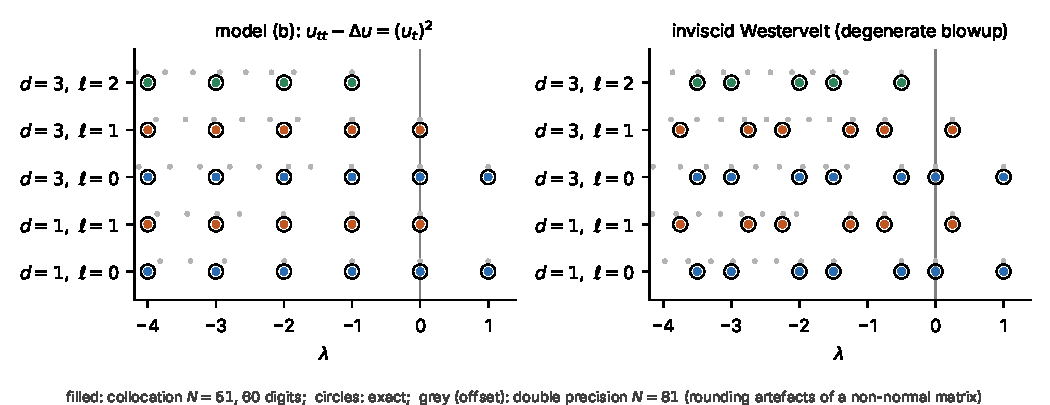
\includegraphics[width=\textwidth]{figures/acou_spectrum.pdf}
\caption{Spectra of the linearisation at the ODE blowup for (RW) (left;
exact: $\lambda=1-j$, $j\ge\ell$) and for the inviscid Westervelt degeneracy
(right; exact: $1-\frac34(\ell+2n)$, $-\frac34(\ell+2n)$). Filled: collocation, $N=61$,
60 digits. Circles: exact. Grey, offset: double precision, $N=81$.}
\label{acou:fig-spec}
\end{figure}

\emph{Tilted blowup in 1D.} We solve (RW) with $u(0)=0$,
$u_t(0)=2/(1+x^2)$ by the characteristic-diamond scheme, which respects the
light cone exactly ($h=10^{-4}$, \texttt{code/acou\_tilt1d.py}). Fitting
$u_t\approx C(x)/(T(x)-t)$ at each $x$ gives a spacelike blowup curve
($\max_{|x|\le1.2}|T'|=0.52$, $T_{\min}=0.5445$). The fitted coefficient
satisfies $|C(x)-(1-T'(x)^2)|\le5\times10^{-4}$, as predicted by
\cref{acou:lem-tilt}. At $x_1=0.8$, with $a=T'(x_1)=0.404$, the rescaled
time derivative $\rho\,u_t(T(x_1)-\rho,x_1+\rho\xi)$ converges to
$(1-a^2)/(1+a\xi)$. The sup-error is $6.1,2.9,1.3,0.64\times10^{-2}$ for
$\rho=0.2,0.1,0.05,0.025$, i.e.\ $O(\rho)$, matching the gap $1$. Its
distance to the ODE profile $1$ stays at $0.41$ (\cref{acou:fig-tilt}).

\begin{figure}[ht]
\centering
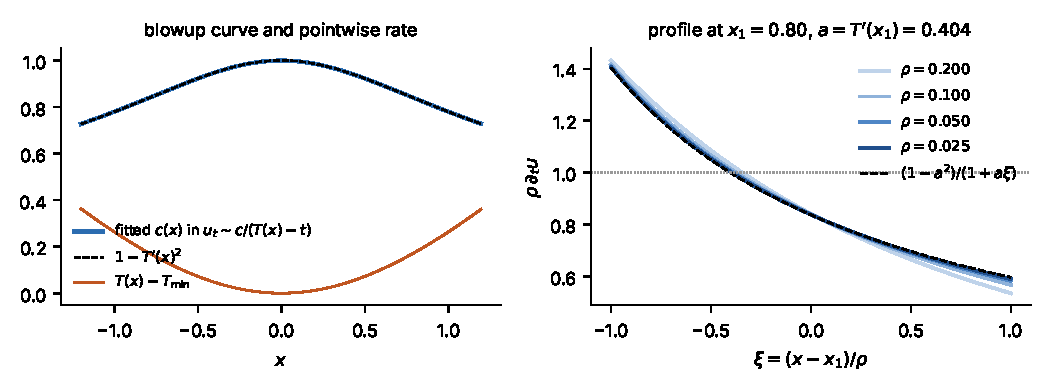
\includegraphics[width=\textwidth]{figures/acou_tilt.pdf}
\caption{(RW) in 1D. Left: blowup curve and pointwise rate coefficient
$C(x)$ versus $1-T'(x)^2$. Right: convergence of $\rho\,\partial_tu$ to the tilted
profile $(1-a^2)/(1+a\xi)$ at a point of the blowup curve with slope $a=0.404$.}
\label{acou:fig-tilt}
\end{figure}

\emph{Westervelt degeneracy in 1D.} We solve \eqref{acou:qeq} ($c=1$, periodic)
with $q(0)=1$, $q_t(0)=-(1+0.2\cos x)$ (\texttt{code/acou\_westervelt1d.py}).
The first degeneracy occurs at $x_0=0$, $T=0.41991$. Fitting
$q^2(t,0)=A\rho+C\rho^{3/2}+D\rho^2+E\rho^{5/2}$ gives $A=2.3092$ and
$C=0.1342$, while the prediction $C=\frac83H/\sqrt A$ with the measured
$H=0.0766$ is $0.1345$, an agreement of $0.2\%$ that is stable under grid
refinement and changes of the fit window. A fit with integer powers only
leaves residuals $2\times10^{4}$ times larger, which confirms the half-integer
expansion predicted by \cref{acou:prop-west}.

\subsection{Summary and caveats}
\label{acou:sub-summary}
\begin{itemize}[nosep]
\item \textbf{(D)} (RW): the linearisation at the ODE blowup is
  \emph{exactly} conjugate to the free wave flow with $s=-1$. Its spectrum
  is $\{1-j\}$, i.e.\ $1-\ell-2n$ and $-\ell-2n$ in the $\ell$-sector, and
  all eigenvalues are semisimple. The neutral $\lambda=0$ modes are the shift
  ($\ell=0$) and the tangents to the exact tilted family $u_{T,a}$
  ($\ell=1$). There is no Jordan block, only a quadratic drift $-|a|^2\tau$
  of $\psi_1$. Radial stability (\cref{acou:thm-rad}) holds with every rate
  $\omega<1$ for $k>\frac d2+2$ (proof sketch).
\item \textbf{(C)} Nonradial stability converges to $u_{T,a}$, not to $u_T$
  (\cref{acou:thm-nonrad}); this is supported by 1D numerics but not proved
  here.
\item \textbf{(K/D)} (NF): explicit via $w=e^{-u}$. The generic first
  blowup is ODE-type with gap $1$ and boosted profiles; non-generic zeros
  give self-similar profiles $-\log P$.
\item \textbf{(D/C)} Westervelt/Kuznetsov ($b=0$): degenerate blowup with
  $p$ bounded and $p_t\sim(T-t)^{-1/2}$, scaling $x\sim(T-t)^{3/4}$, and a
  formal spectrum $\{1-\frac34(\ell+2n)\}\cup\{-\frac34(\ell+2n)\}$. The
  linear structure is Donninger-like, but the nonlinear problem is
  quasilinear and open; it is physically outside the validity of the model.
\item \textbf{(D/C)} The viscous term $b\Delta p_t$ dominates in similarity
  variables, so the light-cone theory does not apply for $b>0$. Heat-type
  blowup is conjectured, but only on picosecond scales.
\item Caveats: semigroup generation on $H^k\times H^{k-1}(B^d)$ for general $d,k$ is
  quoted, not reproved. The nonlinear arguments are sketches. References
  marked \texttt{TODO verify} in the source could not be checked online.
\end{itemize}

\section{Numerical verification}
\label{num:sec}

This section reports an \emph{independent} numerical check of the spectral
claims of \cref{fw:thm-spec} and of the physical picture behind them: that
hyperbolic MEMS touchdown, started from physical data, is governed in the
backward light cone by the ODE profile, at the rate predicted by the
spectral gap. All computations are done from scratch from the
coordinates of \cref{fw:sec}; no formula of the analytic sections is used as
input except as the thing to be compared with. The scripts are listed in
\cref{num:subsec-repro}. In brief:
\begin{itemize}[leftmargin=1.4em,itemsep=1pt]
\item \textbf{Spectra} (\cref{num:subsec-spec}). For all $17$ model/dimension
  combinations and $\ell=0,1,2$ ($46$ sectors) the converged eigenvalues with
  $\operatorname{Re}\lambda\ge-3$ coincide with
  $\{a_1-s-\ell-2n\}\cup\{a_2-s-\ell-2n\}$ (to $5\cdot10^{-20}$ in $30$-digit
  arithmetic) and do not depend on $d$; no other eigenvalue occurs. Double
  precision is \emph{not} sufficient: a spurious branch, which moves to the
  right as $N$ grows, swallows part of the window. Two discrepancies with the hints: \emph{(i)} for MEMS with
  $q=3$ (and for $p=5$) the two families collide and the collision
  eigenvalues are $2\times2$ Jordan blocks, among them the gap eigenvalue
  $\lambda=-1$ for $q=3$; \emph{(ii)} the derivative model is not of the
  potential form \eqref{fw:eig}; its eigenvalues are $\{1-\ell-2n\}\cup\{-\ell-2n\}$.
\item \textbf{MEMS touchdown} (\cref{num:subsec-mems}). From the physical
  data $w(0)=1$, $w_t(0)=0$ in $d=1,2$, with and without damping, the minimum
  of the gap behaves like $c(T-t)^{2/3}$, local exponent $0.66666$ and
  $c=(9\lambda/2)^{1/3}$ recovered to $2\cdot10^{-7}$ ($d=1$), $4\cdot10^{-6}$ ($d=2$);
  the light-cone profile converges to the constant $c$ at the rate
  $(T-t)^{\omega}$, measured $\omega=0.6666\pm0.0001$, in agreement with
  $\omega_0=2/3$; the slowest mode is the spatially constant ``ODE-energy''
  mode $\lambda=-2/3$, the spatial variation decays like $(T-t)^{1}$. Power-law
  fits at moderate gaps ($w_{\min}\ge0.02$) give exponents $0.50$--$0.64$.
\item \textbf{Asymmetric data} (\cref{num:subsec-boost}). At the touchdown
  point the profile converges to the \emph{flat} ODE profile ($a=0$); a
  boosted profile with $a=T'(x_0)\ne0$ appears at the other points $x_0$
  of the blowup curve, which are not physically reached.
\item \textbf{Exponential nonlinearity} in $d=1$ (\cref{num:subsec-exp}):
  convergence with $\omega=1.000$, along the predicted eigenfunction $1-\xi^2$.
\end{itemize}

%-----------------------------------------------------------------------------
\subsection{Spectra of the linearised operators}
\label{num:subsec-spec}

\paragraph{Formulation.}
For $F=|u|^{p-1}u$ and $F=-\lambda w^{-q}$ we use the variables
\eqref{fw:psi}; for $F=e^u$ the logarithmic variables of \cref{fw:sec}; for
the derivative model $u_{tt}-\Delta u=(u_t)^2$, whose ODE solution is
$u=-\log(T-t)$, we set $\psi_1=u+\log(T-t)$, $\psi_2=(T-t)u_t$, which gives
$\partial_\tau\psi_1=-\Lambda\psi_1+\psi_2-1$,
$\partial_\tau\psi_2=\Delta\psi_1-\Lambda\psi_2-\psi_2+\psi_2^2$ with the
fixed point $(0,1)$ (up to the shift $\psi_1\mapsto\psi_1+\text{const}$).
Linearising at the constant fixed point and inserting
$\phi_j=e^{\lambda\tau}|\xi|^\ell Y_\ell(\xi/|\xi|)\,h_j(z)$, $z=|\xi|^2$,
where $\Lambda\mapsto \ell+2z\partial_z$ and
$\Delta\mapsto 4z\partial_z^2+(4\ell+2d)\partial_z$, gives the
eigenvalue problem on $z\in[0,1]$
\begin{equation}\label{num:eig}
\lambda\begin{pmatrix}h_1\\h_2\end{pmatrix}=
\begin{pmatrix}-(\ell+s)-2z\partial_z & 1\\
4z\partial_z^2+(4\ell+2d)\partial_z+V_0 & -(\ell+s+1)-2z\partial_z\end{pmatrix}
\begin{pmatrix}h_1\\h_2\end{pmatrix}
\end{equation}
with $(s,V_0)=(\frac2{p-1},\,ps(s+1))$, $(-\frac2{q+1},\,\frac{2q(q-1)}{(q+1)^2})$,
$(0,2)$ for the power, MEMS and exponential cases; for the derivative
model the $(1,1)$ entry is $-\ell-2z\partial_z$, the $(2,2)$ entry is
$-(\ell-1)-2z\partial_z$ and $V_0=0$.

\paragraph{Discretisation.}
Chebyshev--Gauss--Lobatto collocation in $z\in[0,1]$ with $N+1$ nodes
(Trefethen's differentiation matrix, mapped by $z=(1+x)/2$), applied to
\eqref{num:eig} \emph{without} any boundary condition: at $z=1$ (the light
cone) none is admissible because all characteristics leave the cone, and at
$z=0$ regularity is built into the ansatz $|\xi|^\ell h(|\xi|^2)$ with $h$ a
polynomial. This is a standard eigenvalue problem of size $2(N+1)$ (no
quadratic pencil is needed). It was solved (a) in double precision for
$N=20,40,80$ (and $120$), (b) with \texttt{mpmath} at $30$ digits for $N=12$ and $N=20$,
and (c) exactly, in rational arithmetic, on polynomials of degree $\le5$ (see
below). An eigenvalue is called \emph{converged} if (b) gives the same value
for both $N$ to $10^{-6}$ (simple eigenvalues in fact agree to
$\le5\cdot10^{-15}$; the looser tolerance accommodates the splitting of
Jordan blocks, see \ref{num:D-jordan}).

\paragraph{Why the closed form is reproduced exactly.}
The computations revealed a simple structural fact that we record because it
explains both the agreement and the numerical difficulties.
\begin{proposition}\label{num:prop-tri}
Let $\mathcal P_n$ be the polynomials of degree $\le n$ in $z$. The operator
$\mathbf A_\ell$ on the right of \eqref{num:eig} maps $\mathcal P_n\times\mathcal P_n$
into itself, and in the basis $\{(z^k,0),(0,z^k)\}_{k\le n}$ it is block upper
triangular with diagonal blocks
$\begin{pmatrix}-(\ell+2k+s)&1\\ V_0&-(\ell+2k+s+1)\end{pmatrix}$, $k=0,\dots,n$.
Hence its eigenvalues are exactly $\lambda=a_i-s-\ell-2k$, $i=1,2$, where
$a_{1,2}$ are the roots of $a^2+a-V_0=0$. Collocation with $N+1$ nodes is the
restriction of $\mathbf A_\ell$ to $\mathcal P_N\times\mathcal P_N$, so in exact
arithmetic its eigenvalues are precisely these numbers with $k\le N$.
\end{proposition}
\begin{proof}
$z\partial_z z^k=kz^k$, while $4z\partial_z^2z^k+(4\ell+2d)\partial_zz^k=k(4k-4+4\ell+2d)z^{k-1}$
lowers the degree. The characteristic polynomial of the $k$-th block is
$(\lambda+\ell+2k+s)(\lambda+\ell+2k+s+1)-V_0$.
\end{proof}
The Laplacian (and hence $d$) enters only through the off-diagonal coupling
$k\to k-1$; it decides eigenvectors and Jordan structure, not eigenvalues.
For the derivative model the blocks are
$\begin{pmatrix}-(\ell+2k)&1\\0&-(\ell+2k-1)\end{pmatrix}$, giving
$\lambda\in\{1-\ell-2k\}\cup\{-\ell-2k\}$. The proposition says nothing about
non-polynomial eigenfunctions; that these do not occur for
$\operatorname{Re}\lambda>-\omega_k$ is the content of the connection-formula
argument in \cref{fw:thm-spec}.

\paragraph{Results.} \Cref{num:tab-spec} lists the converged eigenvalues
(46 sectors). Every simple one agrees with the closed form to
$\le5\cdot10^{-20}$, the double ones are discussed in \ref{num:D-jordan}, the
multiplicities are those predicted by \cref{num:prop-tri}, and the lists are
identical for $d=1,2,3$. No eigenvalue outside the closed-form list was found.

\begin{table}[ht]
\centering\small
\begin{tabular}{@{}llllll@{}}
\toprule
model & $(s,V_0)$ & $\ell=0$ & $\ell=1$ & $\ell=2$ ($d\ge2$) & $\omega_0$\\
\midrule
MEMS $q=2$ & $(-\frac23,\frac49)$ & $1,\,-\frac23,\,-1,\,-\frac83,\,-3$ & $0,\,-\frac53,\,-2$ & $-1,\,-\frac83,\,-3$ & $\frac23$\\
MEMS $q=3$ & $(-\frac12,\frac34)$ & $1,\,-1^{J},\,-3^{J}$ & $0,\,-2^{J}$ & $-1,\,-3^{J}$ & $1^{J}$\\
MEMS $q=4$ & $(-\frac25,\frac{24}{25})$ & $1,\,-1,\,-\frac65,\,-3$ & $0,\,-2,\,-\frac{11}5$ & $-1,\,-3$ & $1$\\
$e^u$ & $(0,2)$ & $1,\,-1,\,-2,\,-3$ & $0,\,-2,\,-3$ & $-1,\,-3$ & $1$\\
$u^3$, $d=3$ & $(1,6)$ & $1,\,-1,\,-3$ & $0,\,-2$ & $-1,\,-3$ & $1$\\
$u^5$, $d=3$ & $(\frac12,\frac{15}4)$ & $1,\,-1,\,-3^{J}$ & $0,\,-2$ & $-1,\,-3$ & $1$\\
$u^7$, $d=3$ & $(\frac13,\frac{28}9)$ & $1,\,-1,\,-\frac83,\,-3$ & $0,\,-2$ & $-1,\,-\frac83,\,-3$ & $1$\\
$(u_t)^2$, $d=1,3$ & --- & $1,\,0,\,-1,\,-2,\,-3$ & $0,\,-1,\,-2,\,-3$ & $-1,\,-2,\,-3$ & $1$\\
\bottomrule
\end{tabular}
\caption{Converged eigenvalues with $\operatorname{Re}\lambda\ge-3$ of the
linearisation at the ODE profile (all real), for $d=1,2,3$ (MEMS, $e^u$), $d=3$
(powers), $d=1,3$ (derivative model); in $d=1$ only $\ell=0,1$ (even/odd)
exist. Identical for all $d$. $J$: algebraic multiplicity $2$, geometric
multiplicity $1$ (Jordan block). Last column: gap after removing $\lambda=1$
(and $\lambda=0$, and for $(u_t)^2$ the shift mode $\lambda=0$, $\ell=0$).}
\label{num:tab-spec}
\end{table}

\paragraph{Discrepancies with the closed-form hint.}
\begin{enumerate}[label=(D\arabic*),leftmargin=2.2em,itemsep=1pt]
\item\label{num:D-jordan} \emph{Jordan blocks.} When $a_1-a_2\in2\mathbb N$
  the two families collide. Among the cases considered this happens for MEMS
  $q=3$ ($a_1-a_2=3-\frac4{q+1}=2$): $\lambda=-1-\ell-2n$ is double, and for
  $p=5$ ($a_1-a_2=\frac4{p-1}+3=4$): $\lambda=-3-\ell-2n$. Exact rational
  arithmetic on $\mathcal P_5\times\mathcal P_5$ gives geometric multiplicity
  $1$ in every collision with $\operatorname{Re}\lambda\ge-3$
  (\cref{num:tab-spec}); in $30$-digit arithmetic the double eigenvalue splits
  into a pair at distance $4\cdot10^{-12}$--$7\cdot10^{-10}$ whose mean agrees with
  the closed form to $5\cdot10^{-21}$, the signature of a $2\times2$ block (simple
  eigenvalues are accurate to $10^{-20}$ in the same computation).
  Analytically: at $q=3$, $\lambda=-1$, $\ell=0$ one has $\alpha=-1$, $\beta=0$
  in \eqref{fw:hyp}, so the equation reduces to $z(1-z)h''+ch'=0$, whose only
  polynomial solution is $h=1$. Consequence: for $q=3$ the gap eigenvalue
  $-1$ is \emph{not} semisimple, and the linearised flow on the stable
  subspace decays like $\tau e^{-\tau}$, i.e.\ $(T-t)|\log(T-t)|$; the statement
  ``rate $e^{-\omega\tau}$ for every $\omega<\omega_0$'' is unaffected, but
  $\omega=\omega_0$ is not attained. (This agrees with the analytic treatment
  in \cref{mems:rem-q3}, which was written in parallel.)
\item\label{num:D-deriv} \emph{Derivative model.} \eqref{fw:eig} does not
  apply ($F$ depends on $u_t$); naively taking $s=0$, $V_0=F'(u_T)(T-t)^2=0$ would give
  $\{-\ell-2n\}\cup\{-1-\ell-2n\}$ and miss the time-translation eigenvalue.
  The correct list is $\{1-\ell-2n\}\cup\{-\ell-2n\}$ (\cref{num:prop-tri}),
  i.e.\ the free list with $s=-1$, and it contains the additional symmetry
  eigenvalue $\lambda=0$, $\ell=0$, with eigenfunction $(1,0)$ (the shift
  $u\mapsto u+\text{const}$).
\item\label{num:D-buried} \emph{Space dependence of the list.} The closed
  form is a list of \emph{polynomial} eigenfunctions; whether a listed number
  is an isolated eigenvalue on $\mathcal H^k$ depends on $k$, see the next
  paragraph. For instance $-2/3$ (MEMS, $q=2$) is invisible in the energy
  space $k=1$ when $d=1$.
\end{enumerate}

\paragraph{Eigenfunctions and symmetries.}
For all cases, the computed eigenvector of $\lambda=1$, $\ell=0$ has $h_1$
constant and $h_2/h_1=1+s$ (resp.\ $1$ for $e^u$ and $(u_t)^2$) to $\le2\cdot10^{-9}$,
which is $\partial_T$ of the ODE profile in the variables \eqref{fw:psi}. The
eigenvector of $\lambda=0$, $\ell=1$ is $\phi_1\propto\xi_j$, $h_2/h_1=1+s$, which is
$\partial_a\Psi_a|_{a=0}$ for the boost family \eqref{fw:boost} (for MEMS:
$\partial_a\Psi_a=c\sigma(\xi_j,(1-\sigma)\xi_j)$). For the derivative model
$\lambda=0$, $\ell=0$ has eigenvector $(1,0)$. More generally, for every simple
eigenvalue $\lambda\ge-1.5$ the eigenvector $h_1$ coincides with the
terminating hypergeometric polynomial ${}_2F_1(\alpha,\beta;\frac d2+\ell;z)$ of
\eqref{fw:hyp} and $h_2=(\lambda+s+\Lambda)h_1$, to $\le10^{-7}$ (double
precision, $N=12$, $70$ checks; for the Jordan eigenvalue $-1$ of $q=3$ only to
$3\cdot10^{-5}$, as expected for a defective eigenvalue). In particular the gap mode of MEMS $q=2$ ($\lambda=-\frac23$)
is the \emph{constant} $h_1\equiv1$, $h_2=-\frac43$, which is the
linearisation of the energy of the ODE $w''=-\lambda w^{-2}$: a solution with
energy $E$ near touchdown satisfies
$w=c(T-t)^{2/3}\big(1+\tfrac{9E}{10c^2}(T-t)^{2/3}+\dots\big)$.

\paragraph{The spurious branch and the Sobolev index.}
In double precision the picture is less clean (\cref{num:fig-spec}): only
the top few eigenvalues converge, and the rest form a curve of complex
eigenvalues which moves \emph{to the right} as $N$ grows; for MEMS, $q=2$,
$d=3$, $N=80$ already shifts $-\frac23$ to $-0.6948$, and at $N=120$ this
eigenvalue is swallowed. Across all cases the right edge of the spurious set
is close to $\frac{d-1}2-s-K_N$ with $K_N\in[4,5.2]$, $[3,4]$, $[2.4,3]$,
$[2,2.7]$ for $N=20,40,80,120$ (six cases tested in \texttt{num\_spurious.py}, $s$ replaced by $-1$ for
$(u_t)^2$; for $(u_t)^2$, $d=3$, $N=120$ even the symmetry eigenvalue $0$ is
destroyed), whereas in
$30$-digit arithmetic the same matrices have exactly the closed-form
eigenvalues (black dots in \cref{num:fig-spec}). Since the exact eigenvalues
of the collocation matrix are known (\cref{num:prop-tri}), these are not
discretisation errors but pseudospectral effects of the extreme
non-normality of $\mathbf A_\ell$ (the eigenvectors are nearly parallel
polynomials). They have a clear meaning. The second Frobenius solution at
the light cone behaves like $(1-|\xi|^2)^{\gamma}$, $\gamma=\frac{d-1}2-s-\lambda$, and
it belongs to $H^k(B^d)$ iff $\operatorname{Re}\gamma>k-\frac12$. Hence on
$\mathcal H^k=H^k\times H^{k-1}$ \emph{every} $\lambda$ with
$\operatorname{Re}\lambda<\frac d2-s-k=-\omega_k$ is an eigenvalue
(with the regular-at-$0$ solution as eigenfunction), so the spectrum of $\mathbf L$ on $\mathcal H^k$
contains a half-plane and the growth bound on $\mathcal H^k$ can be no better than $-\omega_k$, consistently with
\cref{fw:thm-spec}. A degree-$N$ polynomial approximates $(1-z)^\gamma$ to
accuracy $\approx N^{-2\operatorname{Re}\gamma}$, so in working precision
$\varepsilon$ the matrix ``sees'' this continuum for
$\operatorname{Re}\gamma\gtrsim\log(1/\varepsilon)/(2\log N)$: the spurious
curve is the continuum of an effective, $N$- and $\varepsilon$-dependent
Sobolev index, and its edge tends to $\frac{d-1}2-s$ (the $L^2$-type
threshold) as $N\to\infty$ at fixed $\varepsilon$. Two practical
consequences: (a) eigenvalue computations of this type must be done in
extended precision or with a convergence check in $N$, and more resolution
in double precision is \emph{worse}; (b) to see the gap $\omega_0$ in
$\mathcal H^k$ one needs $k\ge\frac d2-s+\omega_0$, i.e.\ $k\ge2,3,3$ for MEMS
$q=2$ in $d=1,2,3$, $k\ge2,2,3$ for $e^u$, $k\ge2$ for $u^3,u^5$ and $k\ge3$
for $u^7$ in $d=3$, and $k\ge3$ ($d=1$), $k\ge4$ ($d=3$) for $(u_t)^2$.

\begin{figure}[ht]
\centering
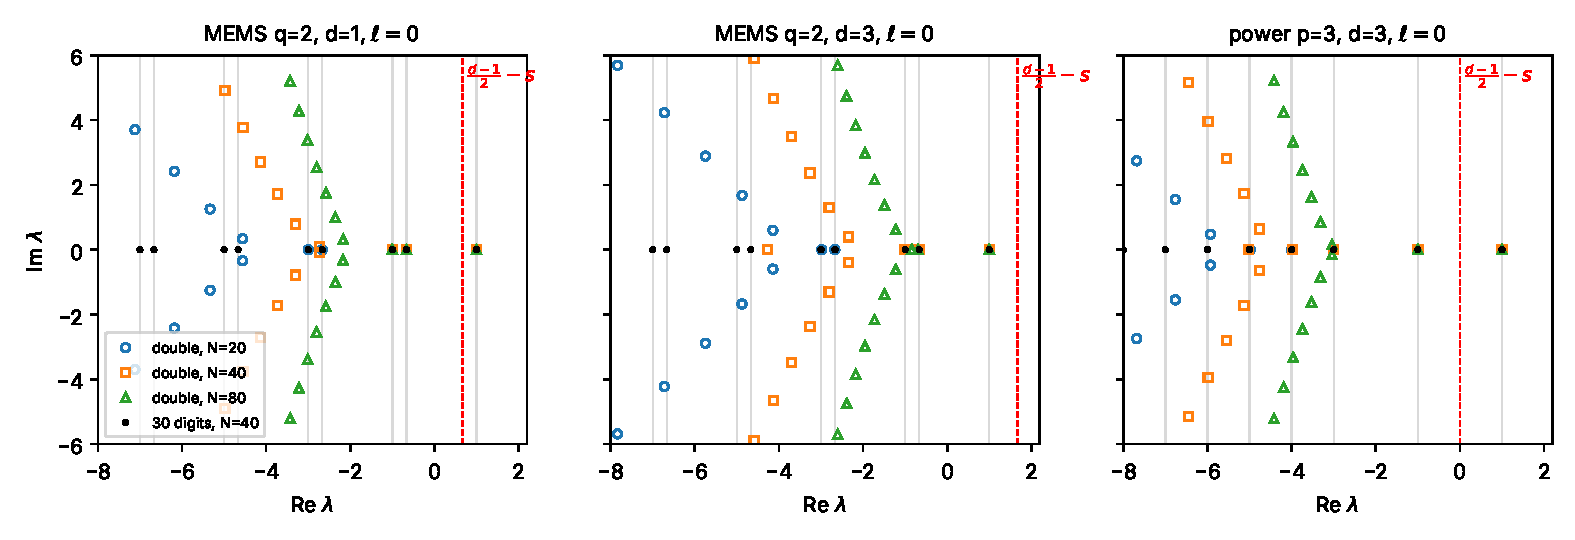
\includegraphics[width=\textwidth]{figures/num_spectra.pdf}
\caption{Eigenvalues of the collocation matrix of \eqref{num:eig}, $\ell=0$.
Coloured: double precision, $N=20,40,80$. Black dots: $30$-digit arithmetic,
$N=32$, which reproduce the closed form (grey vertical lines) exactly. The
red dashed line is $\operatorname{Re}\lambda=\frac{d-1}2-s$; the spurious
curve approaches it as $N$ grows.}
\label{num:fig-spec}
\end{figure}

%-----------------------------------------------------------------------------
\subsection{Touchdown dynamics of the hyperbolic MEMS equation}
\label{num:subsec-mems}

\paragraph{Problem and parameters.} We solve
\begin{equation}\label{num:mems}
  w_{tt}+\gamma w_t-\Delta w=-\lambda w^{-2}\ \text{ in }\Omega,\qquad
  w=1\text{ on }\partial\Omega,\qquad w(0)=1,\ w_t(0)=0,
\end{equation}
for $\Omega=(-1,1)$ and for radial solutions on the unit disk, with
$\gamma\in\{0,1\}$. The static pull-in value (fold of $\Delta w=\lambda w^{-2}$,
$w|_{\partial\Omega}=1$, by shooting) is $\lambda^*=0.35000$ ($d=1$) and $0.78923$
($d=2$); the dynamic threshold, defined as the smallest $\lambda$ with
$\min w<0.05$ before $t=30$, lies in $[0.2895,0.2961]$ ($d=1$, $\gamma=0$),
$[0.3426,0.3492]$ ($d=1$, $\gamma=1$), $[0.6406,0.6492]$ ($d=2$, $\gamma=0$) and
$[0.7438,0.7523]$ ($d=2$, $\gamma=1$) (\texttt{num\_mems\_threshold.py}; for $\gamma=0$
the finite-horizon value is an upper bound for the true threshold). We take
$\lambda=0.5$ ($d=1$) and $\lambda=0.8$ ($d=2$), above the dynamic threshold in all
four cases and small enough that the touchdown time exceeds $1$: for $T\le1$
the solution in $|x|<1-t$ is the ODE solution, and the gap closes
simultaneously on a whole interval (disk), a degenerate situation. With
$T>1$ the boundary has influenced the whole backward light cone of the
touchdown point.

\paragraph{A weak singularity.} The data are incompatible with the boundary
condition at second order ($w_{tt}(0)=-\lambda\ne0=\partial_t^2 1$), so a jump
of $w_{tt}$ travels inwards from $\partial\Omega$ along characteristics. In $d=2$
it focuses at $(t,r)=(1,0)$, i.e.\ \emph{inside} the backward light cone of
the touchdown point. This is physical (a voltage switched on instantaneously),
but it destroys the spectral accuracy of global methods: in a preliminary
test, a Chebyshev method in physical space changed $T$ by $\approx10^{-7}$
between $N=128$ and $N=256$. We
therefore use the following three-stage method.

\paragraph{Method.}
\emph{Stage 1 (physical space, $0\le t\le t_1$).} In $d=1$: leapfrog with
$\Delta t=\Delta x$ (exact for the free wave equation; the singular
characteristics are grid diagonals), on $M=4000,8000,16000$ cells, combined by
Richardson extrapolation; in $d=2$: the conservative second-order leapfrog for
$r^{-1}\partial_r(r\partial_r)$ with $\Delta t=\Delta r/2$, $M=4000,8000$, followed
by a least-squares fit of $w(t_1,\cdot)$, $w_t(t_1,\cdot)$ by even Chebyshev
polynomials of degree $40$ on $[0,R_0]$, which removes grid-scale noise
($\approx10^{-4}$ in $w_t$) left by the focusing; $R_0$ is kept below the
position of the singular front. The switching time $t_1$ is the multiple of
$0.01$ just before $\min w=0.3$.

\emph{Stage 2 (light cone of $(T,0)$, $t\ge t_1$).} With
$\tau=-\log\frac{T-t}{T-t_1}$, $\xi=\frac{x}{T-t}$, $\psi_1=(T-t)^{-2/3}w$,
$\psi_2=(T-t)^{1/3}w_t$,
\begin{equation}\label{num:simmems}
  \partial_\tau\psi_1=-\Lambda\psi_1+\tfrac23\psi_1+\psi_2,\qquad
  \partial_\tau\psi_2=\Delta\psi_1-\Lambda\psi_2-\tfrac13\psi_2-\lambda\psi_1^{-2}
  -\gamma(T-t_1)e^{-\tau}\psi_2 ,
\end{equation}
discretised by Chebyshev collocation in $\xi\in[-1,1]$ ($21$ nodes, $d=1$) or
in $z=|\xi|^2\in[0,1]$ ($17$ nodes, radial), without boundary conditions, and
integrated with an adaptive 8th-order Runge--Kutta method (DOP853, relative
tolerance $10^{-12}$). Initial data are interpolated from stage 1 (local
10-point Lagrange interpolation in $d=1$, the even fit in $d=2$). The ODE
profile is $(\psi_1,\psi_2)=(c,-\frac23c)$, $c=(9\lambda/2)^{1/3}$.

\emph{Stage 3 ($T$ by bisection).} If $T$ is too large, the solution quenches
inside the cone at finite $\tau$ ($\min\psi_1\to0$); if $T$ is too small,
$\psi_1\sim e^{2\tau/3}w(T,0)\to\infty$. Bisection is run to relative width
$4\cdot10^{-16}$. Because of the time-translation mode $e^{\tau}$, the two
trajectories belonging to the ends of the final bracket separate eventually;
all rates are measured only on the $\tau$-window where their values of
$W(\tau,0)-c$ agree to $0.1\%$.

\emph{Independent check.} Stage 1 alone, continued in physical space
($M=16000$, resp.\ $8000$) down to $\min w=0.02$ (resp.\ $0.03$), and fitted
with $T$ as a free parameter.

\paragraph{Results.} In all four cases the minimum of $w$ is attained at the
centre; the same holds for all values tested in \texttt{num\_mems\_threshold.py}
($\lambda=0.35,0.5,1$ for $d=1$, $\lambda=0.7,\dots,1.2$ for $d=2$, $\gamma=0,1$): no
off-centre or ring quenching occurred. The
main numbers are collected in \cref{num:tab-mems}; \cref{num:fig-mems,num:fig-mems2}
show the evolution.

\begin{table}[ht]
\centering\small
\setlength{\tabcolsep}{4pt}
\begin{tabular}{@{}lccccccc@{}}
\toprule
case & $T$ & $\min(T-t)$ & $\omega_{\rm fit}$ & $\omega$, $c$ free & $C_\infty/c-1$ & $\frac{\psi_2+\frac23c}{\psi_1-c}$ & rate of $\operatorname{osc}W$\\
\midrule
$d=1$, $\gamma=0$ & $1.75194263316$ & $1.2\cdot10^{-7}$ & $0.66663$ & $0.6649$ & $2.1\cdot10^{-7}$ & $-1.3319$ & $0.995$\\
$d=1$, $\gamma=1$ & $2.40507517419$ & $4.0\cdot10^{-8}$ & $0.66662$ & $0.6642$ & $2.6\cdot10^{-7}$ & $-1.3318$ & $0.994$\\
$d=2$, $\gamma=0$ & $1.41984985$ & $1.8\cdot10^{-7}$ & $0.66666$ & $0.6627$ & $1.2\cdot10^{-6}$ & $-1.3312$ & $0.991$\\
$d=2$, $\gamma=1$ & $2.214154$ & $2.6\cdot10^{-7}$ & $0.66655$ & $0.6597$ & $3.8\cdot10^{-6}$ & $-1.3296$ & $0.985$\\
\midrule
prediction & & & $\frac23$ & $\frac23$ & $0$ & $-\frac43$ & $1$\\
\bottomrule
\end{tabular}
\caption{Hyperbolic MEMS touchdown, $q=2$, $\lambda=0.5$ ($d=1$), $\lambda=0.8$
($d=2$). $T$: bisection (digits shown are stable under changes of the
light-cone resolution; in $d=2$ the stage-1 resolution changes $T$ by
$8\cdot10^{-9}$ ($\gamma=0$) and $2\cdot10^{-7}$ ($\gamma=1$)). $\min(T-t)$: end of
the validity window. $\omega_{\rm fit}$: fit of $W(\tau,0)-c$ by
$Ae^{-\omega\tau}+Be^{-\tau}+Ce^{-4\tau/3}$ on $\tau\ge3$ ($e^{-4\tau/3}$ is the
square of the gap mode); without the $C$ term one gets $0.6656$, $0.6651$,
$0.6643$, $0.6625$. Next column: fit $W(\tau,0)=C_\infty+Ae^{-\omega\tau}+Be^{-\tau}$
with $c$ unknown. Ratio column: at the end of the window, $\xi=0$. Last
column: decay rate of $\max_\xi W-\min_\xi W$.}
\label{num:tab-mems}
\end{table}

\begin{enumerate}[label=(\roman*),leftmargin=2em,itemsep=2pt]
\item \emph{Exponent and constant.} With $T$ from the bisection, the local
  slope $d\log w_{\min}/d\log(T-t)$ for $T-t<10^{-6}$ is $0.666656$,
  $0.666655$, $0.666640$, $0.666627$, and $w_{\min}(T-t)^{-2/3}\to c$; leaving $c$
  free in the fit returns $c=(9\lambda/2)^{1/3}$ to $2\cdot10^{-7}$ ($d=1$) and
  $4\cdot10^{-6}$ ($d=2$). The approach is slow: the relative correction is
  $(A/c)(T-t)^{2/3}$ with $A/c=-1.44,-2.18,-2.82,-3.87$, so that $w_{\min}$ is
  within $1\%$ of $c(T-t)^{2/3}$ only for $T-t\lesssim10^{-4}$--$6\cdot10^{-4}$, i.e.\
  $w_{\min}\lesssim3\cdot10^{-3}$--$10^{-2}$ (\cref{num:fig-mems}, middle;
  \cref{num:fig-mems2}, right).
  Consequently, the independent physical-space fits over $w_{\min}\in[0.02,0.25]$
  with $T$ free give $\beta=0.596,0.559,0.545,0.500$ for $w=C(T-t)^\beta$, and
  still $\beta=0.644,0.627,0.614,0.589$ if the correction
  $(1+e(T-t)^{2/3})$ is included; their $T$ deviates from the bisection value
  by $8\cdot10^{-5}$--$1.4\cdot10^{-3}$. \emph{Exponents read off from moderate gaps are
  biased low}; this matters when comparing with experiments or with
  simulations that stop at $w_{\min}=O(10^{-2})$.
\item \emph{Light-cone profile.} $W(t,\xi)=(T-t)^{-2/3}w(t,(T-t)\xi)$ converges
  uniformly on $|\xi|\le1$ to the constant $c$ (\cref{num:fig-mems2}, left), with
  $\|W-c\|_\infty\sim(T-t)^{\omega}$, $\omega=0.6666\pm0.0001$ when the
  quadratic term of the gap mode is included, in agreement with
  $\omega_0=\frac23$. The deviation is, to leading order, the spatially
  \emph{constant} eigenfunction $(1,-\frac43)$ of $\lambda=-\frac23$ (ratio column),
  i.e.\ the ODE-energy mode: $W(t,0)-c\approx A(T-t)^{2/3}$ with $A<0$, as for an
  ODE solution of negative energy. The spatial oscillation $\operatorname{osc}_\xi W$
  decays faster, like $(T-t)^{1}$, which is the next even eigenvalue
  $\lambda=-1$ (eigenfunction $1+\frac{|\xi|^2}{3d}$ in the first component). Damping does not change
  the rate (it enters at order $e^{-\tau}$), only the coefficients.
\end{enumerate}

\begin{figure}[ht]
\centering
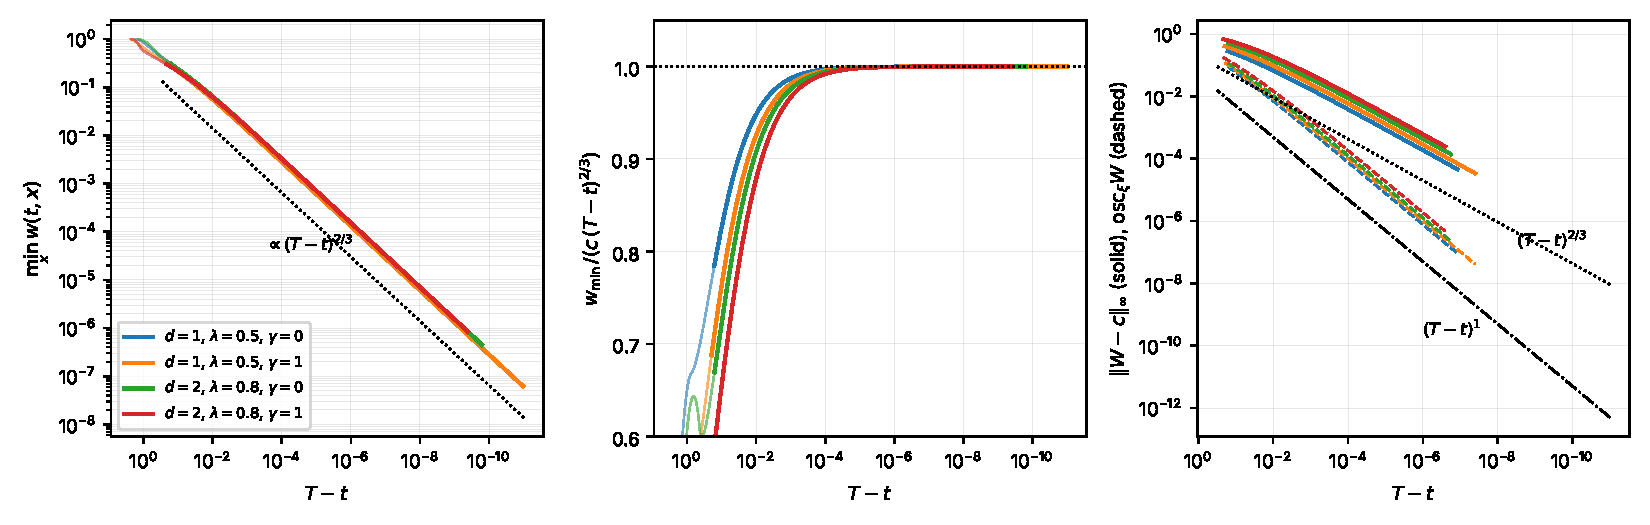
\includegraphics[width=\textwidth]{figures/num_mems_touchdown.pdf}
\caption{Hyperbolic MEMS touchdown. Left: $\min_xw$ versus $T-t$ (thin:
physical-space leapfrog alone; thick: light-cone evolution). Middle:
$w_{\min}/(c(T-t)^{2/3})$. Right: $\|W-c\|_{L^\infty(|\xi|\le1)}$ (solid) and
$\max_\xi W-\min_\xi W$ (dashed) with the slopes $\frac23$ and $1$.}
\label{num:fig-mems}
\end{figure}

\begin{figure}[ht]
\centering
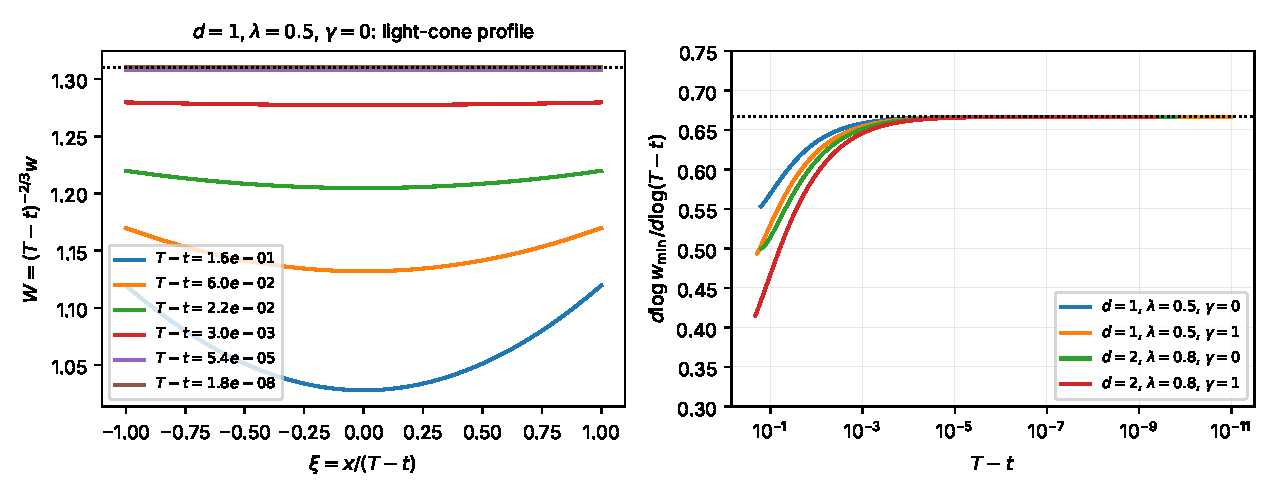
\includegraphics[width=0.85\textwidth]{figures/num_mems_profiles.pdf}
\caption{Left: light-cone profiles $W(t,\cdot)$, $d=1$, $\lambda=0.5$, $\gamma=0$,
flattening to $c$ (dotted). Right: local exponent $d\log w_{\min}/d\log(T-t)$.}
\label{num:fig-mems2}
\end{figure}

\paragraph{Comparison with \cite{GimperleinHeLacey2022}.} That work studies
the same equation formally and numerically for radial data and predicts
quenching at the origin with the ODE law $\kappa(T-t)^{2/(q+1)}$, stability of
this profile up to time translation, and instability of the non-trivial
self-similar profiles (as summarised in \cref{lit:sec}; we could not access
the full text, so we do not compare individual numbers). Our computations
agree on all three qualitative points: quenching at the centre, exponent
$\frac23$ and constant $(9\lambda/2)^{1/3}$, and convergence to the ODE profile
at the spectral-gap rate; starting from physical data we never observed an
approach to a non-trivial profile. Our computations add two quantitative points: the
identification of the slowest correction as the ODE-energy mode, and the
warning in (i) about pre-asymptotic exponents.

%-----------------------------------------------------------------------------
\subsection{Asymmetric data: flat or boosted profile?}
\label{num:subsec-boost}

The boosted family \eqref{fw:boost} reads, for MEMS,
$w=c(1-a^2)^{-\sigma/2}(T-t+a\cdot x)^{\sigma}$, i.e.\
$W_a(\xi)=c(1-a^2)^{-\sigma/2}(1+a\cdot\xi)^{\sigma}$ in the light cone. We
verified by substitution (\texttt{sympy}, $q=2,3,4$) that it is an exact
solution: with $Z=T-t+a\cdot x$, $w_{tt}-\Delta w=(1-|a|^2)W''(Z)$ and
$(1-|a|^2)W''+\lambda W^{-q}\equiv0$ for $W=c(1-|a|^2)^{-\sigma/2}Z^\sigma$.
As a test of the solver, $W_{0.4}$ stays stationary under \eqref{num:simmems}
to $4\cdot10^{-10}$ over $\tau\in[0,12]$ (the residual growth is the
time-translation instability seeded by round-off).

Since $W_a$ vanishes on the line $t=T+a(x-x_0)$, a boosted limit at a point
$x_0$ of the blowup curve $x\mapsto T(x)$ should have $a=T'(x_0)$ (in one
dimension and for power nonlinearities this is the Merle--Zaag picture of
non-characteristic points \cite{MerleZaag2007}); at the \emph{first}
touchdown point, $T'(x^*)=0$, and the profile should be flat. To test this we
took the asymmetric data $w(0,x)=1+0.25\,x(1-x^2)$, $w_t(0)=0$, $\lambda=0.5$,
$\gamma=0$, $d=1$, and computed by bisection, for twelve base points $x_0$, the
blowup time $T(x_0)$ of the backward light cone of $(T,x_0)$; this is the
blowup curve, which exists (and is $1$-Lipschitz) also beyond the first
touchdown, although the physical problem ends there.

\paragraph{Results.} The blowup curve (\cref{num:fig-boost}, left) is smooth
with a non-degenerate minimum at $x^*=0.00860$, $T(x^*)=1.7356545138$,
$T''(x^*)\approx1.76$: the asymmetric data shift the touchdown point (slightly
to the right, although the initial gap is smaller on the left), and
$|T'|\le0.23<1$ on the computed range, i.e.\ these points are non-characteristic. A degree-6 fit
through the twelve values of $T(x_0)$ (residual $7\cdot10^{-9}$; changing the
degree alters $T'$ by $<5\cdot10^{-5}$) gives $T'(x_0)$. At five base points the
boost parameter $a(t)$ of the light-cone profile, defined by
$W(t,1)/W(t,-1)=\big(\frac{1+a}{1-a}\big)^{2/3}$, converges, and at
$T(x_0)-t\approx6\cdot10^{-9}$:
\begin{center}\small
\begin{tabular}{@{}rrrrr@{}}
\toprule
$x_0-x^*$ & $a$ (light cone) & $T'(x_0)$ & $\|W-W_a\|_\infty$ & rate of $\|W-W_a\|_\infty$\\
\midrule
$0$ & $-0.0000112$ & $-0.0000116$ & $7.3\cdot10^{-6}$ & $0.654$\\
$-0.12$ & $-0.1981299$ & $-0.1981283$ & $6.2\cdot10^{-6}$ & $0.649$\\
$-0.06$ & $-0.1021323$ & $-0.1021325$ & $6.2\cdot10^{-6}$ & $0.650$\\
$+0.06$ & $+0.1096470$ & $+0.1096483$ & $8.1\cdot10^{-6}$ & $0.649$\\
$+0.12$ & $+0.2274879$ & $+0.2274882$ & $8.7\cdot10^{-6}$ & $0.647$\\
\bottomrule
\end{tabular}
\end{center}
(the rate is a straight-line fit of $\log\|W-W_{a(t)}\|_\infty$ against $\tau$ for $\tau>3$, which
is biased low by the same pre-asymptotic corrections as the two-term fits
quoted in the caption of \cref{num:tab-mems}; the window ends where the
trajectories for the two ends of the $T$-bracket differ by $10\%$ of
$\|W-W_a\|_\infty$). Thus $a_\infty=T'(x_0)$ to within $2\cdot10^{-6}$ at every
base point, and \emph{at the touchdown point the limit profile is the flat ODE
profile}: the residual $a\approx-1.1\cdot10^{-5}$ there is exactly $T'$ at
our numerical $x^*$, which is off by $\approx7\cdot10^{-6}$. Boosted
profiles appear only at points $x_0\neq x^*$ of the blowup curve, which the
physical (quenched) solution never reaches. For the stability theory this
means: the boost parameters must be modulated (the limit $a_\infty$ is not
determined by the symmetry of the data), but at the first touchdown point the
modulated parameter converges to $0$.

\begin{figure}[ht]
\centering
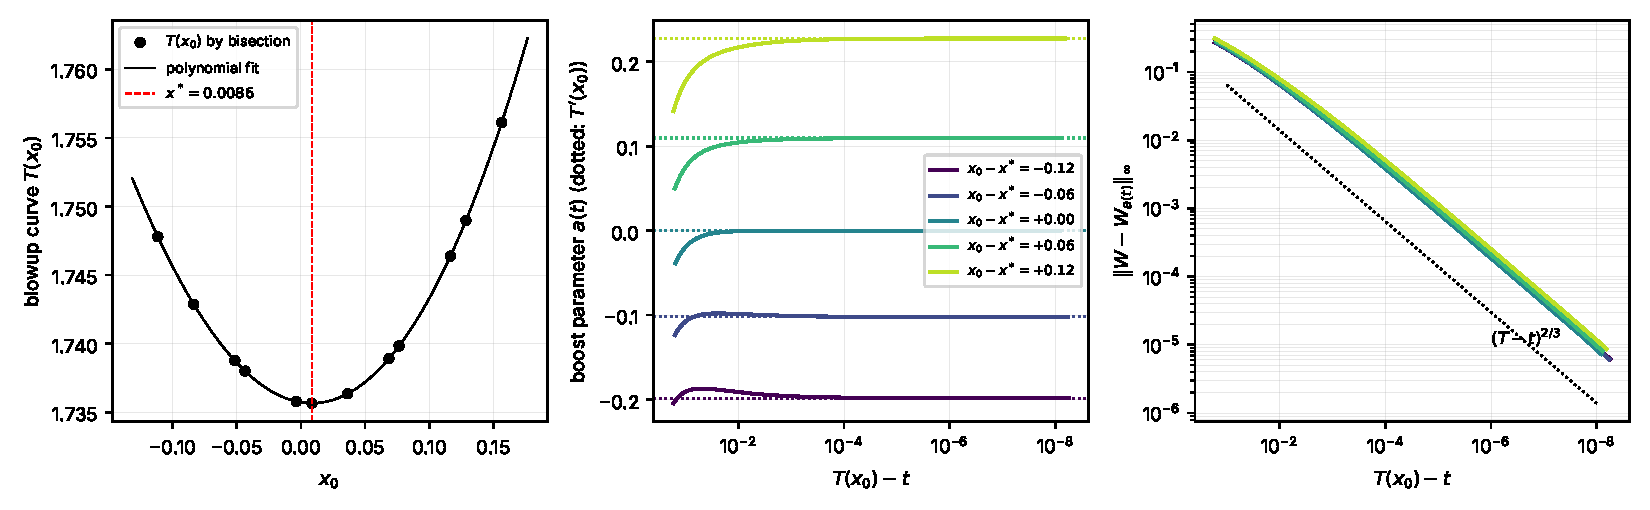
\includegraphics[width=\textwidth]{figures/num_mems_boost.pdf}
\caption{Asymmetric data $w(0,x)=1+0.25\,x(1-x^2)$, $\lambda=0.5$, $d=1$. Left:
blowup curve $T(x_0)$ (bisection) and the touchdown point $x^*$. Middle:
boost parameter of the light-cone profile at five base points versus
$T(x_0)-t$; dotted: $T'(x_0)$. Right: distance to the boosted family.}
\label{num:fig-boost}
\end{figure}

%-----------------------------------------------------------------------------
\subsection{Exponential nonlinearity in one dimension}
\label{num:subsec-exp}

The same three-stage method was applied to $u_{tt}-u_{xx}=e^u$ on $(-1,1)$,
$u=0$ at $x=\pm1$, $u(0)=u_t(0)=0$ (\texttt{num\_exp\_touchdown.py}; here
$\psi_1=u+2\log(T-t)$, $\psi_2=(T-t)u_t$, fixed point $(\log2,2)$; bisection
flags: $\max\psi_1\to\infty$ if $T$ is too large, $\psi_1\to-\infty$ if too small).
Blowup occurs at $x=0$ at $T=2.91356673558862$ (switching time $t_1=2.68$; the
value changes by $1.7\cdot10^{-13}$ if the light-cone resolution is increased).
Here \cref{num:tab-spec} predicts, in the even sector, the eigenvalues $1$
(time translation), $-1$ with eigenfunction $(1-\xi^2,\,-(1+\xi^2))$ and $-2$
(constant, the ODE energy mode), so the deviation should decay like
$(T-t)^1$ with the shape $1-\xi^2$. Measured: $\omega=1.00000$ (fit
$Ae^{-\omega\tau}+Be^{-2\tau}$ on $\tau\in[3,12.1]$; late-window slope
$0.99996$); at $T-t=1.3\cdot10^{-6}$ the deviation is
$\psi_1-\log2\propto 1-1.0004\,\xi^2+5\cdot10^{-7}\xi^4$, and
$(\psi_2-2)/(\psi_1(\cdot,0)-\log2)=-1.0008$ at $\xi=0$ and $-2.0012$ at $\xi=\pm1$
(predicted $-1$, $-2$; the small offsets are the time-translation mode
$(1,1)$ seeded by round-off); see \cref{num:fig-exp}. Note that, unlike MEMS with
$q=2$, the slowest mode is \emph{not} spatially constant: the ODE energy mode
($-2$) is faster than the first spatial mode ($-1$).

\begin{figure}[ht]
\centering
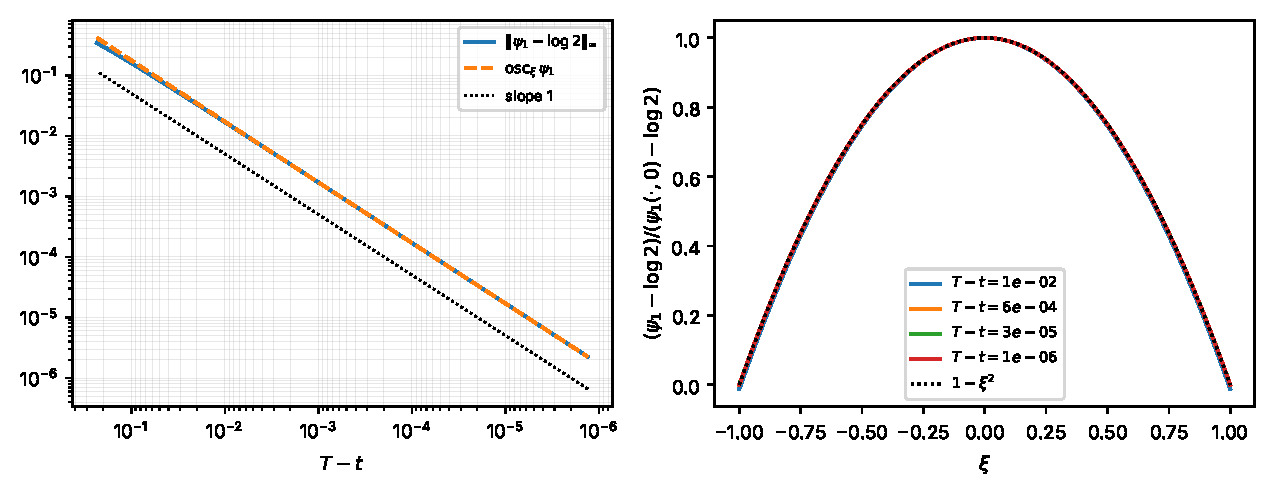
\includegraphics[width=0.8\textwidth]{figures/num_exp_touchdown.pdf}
\caption{$u_{tt}-u_{xx}=e^u$: deviation from the ODE profile in the light cone
(left) and its shape (right), normalised at $\xi=0$, versus $1-\xi^2$.}
\label{num:fig-exp}
\end{figure}

%-----------------------------------------------------------------------------
\subsection{Discrepancies, caveats and reproducibility}
\label{num:subsec-repro}

\paragraph{Discrepancies with the analytic hints.}
\begin{enumerate}[leftmargin=1.6em,itemsep=1pt]
\item MEMS $q=3$ (and $p=5$): Jordan blocks at the collisions of the two
  eigenvalue families, including the gap eigenvalue $\lambda=-1$ for $q=3$
  (\ref{num:D-jordan}). Semisimplicity, which the hint asks to check, holds for
  $\lambda=1$ and $\lambda=0$ in all cases, but fails there.
\item The derivative model is outside the scope of \eqref{fw:eig}
  (\ref{num:D-deriv}); its spectrum is the free one with $s=-1$.
\item The closed-form lists are exact for polynomial eigenfunctions, but their
  meaning as $\mathcal H^k$-spectra requires $k\ge\frac d2-s+\omega_0$
  (\ref{num:D-buried}); the energy space is too small for MEMS in every
  dimension.
\item No discrepancy in the nonlinear tests: exponent $\frac23$, constant
  $(9\lambda/2)^{1/3}$, rate $\omega_0=\frac23$ (MEMS), $\omega_0=1$ ($e^u$) and flat
  limit at the touchdown point are all confirmed. The hint that the profile
  ``can also converge to a boosted profile'' is correct only at points $x_0\neq x^*$
  of the blowup curve, with $a=T'(x_0)$.
\end{enumerate}

\paragraph{Caveats.}
\begin{itemize}[leftmargin=1.4em,itemsep=1pt]
\item The eigenvalue computations only probe polynomial eigenfunctions
  (\cref{num:prop-tri}); absence of non-polynomial eigenfunctions in
  $\operatorname{Re}\lambda>-\omega_k$ rests on the connection-formula
  argument of \cref{fw:thm-spec}, not on numerics.
\item The nonlinear simulations cover one $\lambda$ per geometry, $q=2$, and
  data at rest; the light-cone stage is spectrally accurate, but the data at
  $t_1$ carry errors of $10^{-10}$--$3\cdot10^{-8}$ ($d=1$) and up to $10^{-7}$
  ($w$) and $2\cdot10^{-5}$ ($w_t$) in $d=2$ because of the corner singularity;
  these shift $T$ (by up to $2\cdot10^{-7}$ in $d=2$) but not the measured rates.
\item Rates are measured on windows of $12$--$17$ units of $\tau$ (5--7 decades
  of $T-t$), limited by the time-translation instability amplifying
  integration errors of size $\approx10^{-14}$.
\item The dynamic pull-in values for $\gamma=0$ are finite-horizon ($t\le30$) values.
\item We could not access the full text of \cite{GimperleinHeLacey2022}
  (network restrictions); the comparison above is with the summary of that
  work in \cref{lit:sec}.
\end{itemize}

\paragraph{Reproducibility.} All scripts run from the project root with
\texttt{python3 code/<name>.py} (numpy, scipy, sympy, mpmath, matplotlib);
times are wall-clock times on a shared 4-core machine.
\begin{center}\small
\begin{tabular}{@{}lll@{}}
\toprule
script & output & time\\
\midrule
\texttt{num\_spectra.py} & \cref{num:tab-spec}, \cref{num:fig-spec}, eigenvector checks & $\approx4$ min\\
\texttt{num\_spurious.py} & spurious-branch edges $K_N$ (\cref{num:subsec-spec}) & $<1$ min\\
\texttt{num\_mems\_threshold.py} & pull-in values, location of the minimum & $<1$ min\\
\texttt{num\_mems\_touchdown.py} & \cref{num:tab-mems}, \cref{num:fig-mems,num:fig-mems2} & $\approx4$--$5$ min\\
\texttt{num\_mems\_boost.py} & \cref{num:fig-boost} and the boost table & $\approx4$ min\\
\texttt{num\_exp\_touchdown.py} & \cref{num:fig-exp} & $<1$ min\\
\texttt{num\_common.py} & shared solvers (not run directly) & ---\\
\bottomrule
\end{tabular}
\end{center}


\section{Summary, engineering consequences and open problems}
\label{concl:sec}

\begin{table}[ht]
\centering\footnotesize
\renewcommand{\arraystretch}{1.25}
\begin{tabularx}{\textwidth}{@{}>{\raggedright\arraybackslash}p{0.17\textwidth}>{\raggedright\arraybackslash}p{0.17\textwidth}>{\raggedright\arraybackslash}p{0.17\textwidth}>{\raggedright\arraybackslash}p{0.14\textwidth}>{\raggedright\arraybackslash}X@{}}
\toprule
Model (application) & Singularity & Non-negative modes & Gap $\omega_0$ & Status in these notes\\
\midrule
Hyperbolic MEMS $w^{-q}$, $q>1$ (electrostatic, vdW, Casimir actuators)
 & touchdown $w\simeq c(T-t)^{\frac2{q+1}}$, flat in cone
 & $1$ (time), $0$ (boosts)
 & $\min\{1,\frac{2(q-1)}{q+1}\}$
 & spectrum proved; stability modulo symmetries and with damping sketched
   (\cref{mems:thm-main,mems:prop-damped}); new\\
MEMS, focused profiles $\psi_n$, $d=2,3$
 & touchdown at a point, $\psi_n(0)\to0$
 & $n$ extra unstable
 & --
 & numerical; \cref{mems:conj-prof}\\
Reduced hyperbolic Gelfand $u_{tt}-\Delta u=\delta e^u$ (Cattaneo heat, FK source)
 & $u\simeq\log\frac2\delta-2\log(T-t)$
 & $1$, $0$
 & $1$ (sharp in $d=1$)
 & stability sketched (\cref{therm:thm:reduced}); 1D exact check via Liouville;
   cf.\ \cite{Kichenassamy1996}\\
Full Cattaneo--FK model
 & $\theta\simeq-\log(T-t)$ (parabolic rate)
 & $1$, $0$ (tilts)
 & $1$ (Jordan block at $-1$)
 & sketched, less checked (\cref{therm:thm:full})\\
Arrhenius source
 & no blowup
 & --
 & --
 & FK blowup only as an intermediate regime\\
Softening foundation / $\varphi^4$ / NLKG, $|u|^{p-1}u$
 & $u\simeq\kappa(T-t)^{-\frac2{p-1}}$
 & $1$, $0$
 & $1$
 & known for $\gamma=m=0$ \cite{Ostermann2024}; lower-order lemma sketched
   (\cref{power:thm-lower-order})\\
Co-rotational wave maps (inertial director dynamics)
 & $2\arctan\frac{r}{\sqrt{d-2}(T-t)}$
 & $1$
 & $\approx0.54$ ($d=3$)
 & known (\cref{geom:thm:d3}); spectrum reproduced numerically\\
Relativistic membranes / Born--Infeld
 & shrinking spheres (lightlike collapse)
 & infinitely many
 & --
 & Donninger method not applicable to spheres; general case open
   (\cref{geom:sec:membranes})\\
Acoustic toy model $u_{tt}-\Delta u=u_t^2$
 & $u\simeq-\log(T-t)$
 & $1$, $0$ (shift; tilts)
 & $1$
 & radial sketched (\cref{acou:thm-rad}); nonradial conjectural; cf.\ \cite{Speck2020}\\
Inviscid Westervelt
 & degeneration $1-2kp\propto(T-t)^{1/2}$
 & $1$, $\frac14$ (tilt), $0$
 & formal
 & quasilinear, open (\cref{acou:sec})\\
\bottomrule
\end{tabularx}
\caption{Status of the models. ``Non-negative modes'' lists the eigenvalues
$\lambda\ge0$ of the linearisation in similarity variables together with
their origin. ``Sketched'' means a proof sketch with all key estimates in
the style of \cite{DonningerSchoerkhuber2017,Ostermann2024}.}
\label{concl:tab}
\end{table}

\subsection{What the analysis says about the devices}
\begin{enumerate}[leftmargin=1.5em]
\item \emph{Rates are universal and robust.} Once inertia is retained, the
final approach to touchdown or runaway is governed by the spatially
homogeneous ODE. For the Coulomb MEMS force the gap closes like
$(9\lambda/2)^{1/3}(T-t)^{2/3}$, against $(3\lambda(T-t))^{1/3}$ in the
parabolic (overdamped) model. Damping, restoring forces and smooth variations
of the permittivity change only lower-order corrections. They decay in
similarity variables, so the hyperbolic rate is the true terminal one even
for strongly damped devices. The parabolic rate is at most an intermediate
regime.
\item \emph{The terminal profile is flat.} In the backward light cone the
stable profile is constant (or a Lorentz-tilted constant). Touchdown
therefore occurs along a spacelike hypersurface $t=T^*(x)$, not at an
isolated point as in the parabolic theory. Focused, point-like touchdown
profiles exist for $d=2,3$ but are unstable. A generic device is not expected
to show them.
\item \emph{Boundaries do not matter locally.} The results are local in the
light cone of the singular point. Clamping conditions, the geometry of the
device and far-away material parameters enter only through the touchdown
time $T^*$ and the tilt $a^*$.
\item \emph{Which singularity actually forms is model-dependent.} The full
Maxwell--Cattaneo thermal-explosion model blows up at the \emph{parabolic}
logarithmic rate, not at the hyperbolic one of the frequently used reduced
model. Arrhenius kinetics removes the blowup altogether. Viscous nonlinear
acoustics leaves the light-cone setting entirely.
\end{enumerate}

\subsection{Open problems suggested by these notes}
\begin{enumerate}[leftmargin=1.5em]
\item Turn the proof sketches of
\cref{mems:thm-main,mems:prop-damped,therm:thm:reduced} into complete
proofs. The new ingredients relative to \cite{Ostermann2024} are the
negative scaling exponent (finite-rank splitting of the free operator,
\cref{mems:lem-free}) and the need to stay away from $w=0$, which the
$L^\infty$ control gives.
\item Prove the existence of the focused MEMS profiles $\psi_n$ in $d=2,3$
(\cref{mems:conj-prof}) and determine their co-dimension. A shooting argument
around the singular static solution $A|x|^{2/(q+1)}$, as in
\cite{BizonMaisonWasserman2007}, looks feasible.
\item Go beyond the light cone: regularity of the touchdown hypersurface,
$a^*=\nabla T^*$, and the hyperboloidal approach of
\cite{BiernatDonningerSchoerkhuber2021,ChenEtAl2024} for MEMS.
\item Models not covered by the method in its present form: MEMS plates
($\Delta^2$, no light cone), nonlocal MEMS, the full Cattaneo model in
higher regularity, and the quasilinear problems (Westervelt degeneration,
membranes).
\item Compare the rigorous picture of \cref{mems:sec} in detail with the
formal analysis and numerics of \cite{GimperleinHeLacey2022,He2021}. This
could not be done here because the paper was not accessible.
\end{enumerate}


\bibliographystyle{abbrv}
\bibliography{bib/all}

\end{document}
